\documentclass{sbthesis}
\usepackage{graphicx}
\usepackage{listings}
\usepackage{color} % color
\usepackage{amsmath}
\usepackage{breqn}
\definecolor{listinggray}{gray}{0.9}

% \IncludeFig{caption}{label}{file}{scale}
\newcommand{\IncludeFig}[4]{
  \begin{figure}[h]
    \centering
    \includegraphics[scale=#4]{#3}
    \caption{#1}
    \label{#2}
  \end{figure}
}

% \Ccode{title}{label}{file}
\newcommand{\Ccode}[3]{
  \lstset{language=c}
  \lstset{basicstyle=\footnotesize}
  \lstset{backgroundcolor=\color{listinggray},rulecolor=\color{blue}}
  \lstset{linewidth=\textwidth, xleftmargin=0pt, xrightmargin=0pt}
  \lstset{commentstyle=\textit, stringstyle=\upshape,showspaces=false}
  \lstset{frame=tb}
  \lstinputlisting[caption={#1},label={#2}]{#3}
}

\newcommand{\Matlab}[3]{
  \lstset{language=matlab}
  \lstset{basicstyle=\footnotesize}
  \lstset{backgroundcolor=\color{listinggray},rulecolor=\color{blue}}
  \lstset{linewidth=\textwidth, xleftmargin=0pt, xrightmargin=0pt}
  \lstset{commentstyle=\textit, stringstyle=\upshape,showspaces=false}
  \lstset{frame=tb}
  \lstinputlisting[caption={#1},label={#2}]{#3}
}

\title{A New Phantom and Gradient Isocenter Estimation for MRI Distortion Correction}
\author{Zongqi Cai}
\Department
\EmailAddress{caiz@csusb.edu}
\Advisor{Keith Evan Schubert}
\Committee*{Kay Zemoudeh}{Haiyan Qiao}{Reinhard Schulte}{}
\CSUSBDate{July 2013}
\Copyright

\AbstractText{abstract contents}
\AcknowledgementText{}
\DedicationText{To Zel and Septimus.}

\NoTables
\NoFigures

\begin{document}
\Thesis

\Chapter{Introduction}
\label{introduction}
\section{Thesis Overview}

Magnetic resonance imaging (MRI) provides an excellent modality for distinguishing different tissues 
in the human body, which makes 
this modality essential for medical applications. MRI can also be used for treatment planning of 
medical procedures that require a great degree of geometrical accuracy such as  
functional radiosurgery~\cite{Kond99}. Unfortunately, the accuracy of MRI for medical targeting applications 
is compromised by the presence of geometric distortions such as non-linearities of the magnetic gradient 
fields or inhomogeneities of the scanner main field 
~\cite{Dor05,LSS06a,LSS06b,LSS08a,LSS08b,Lang99,Wang04a,Wang04b}. 
Gradient nonlinearities can cause over 2mm of distortion to the location of features in the 
image~\cite{LSS08b,Lang99}.

% Modern MRI scanners have built-in distortion correction algorithms, that rely on knowledge of the magnetic 
% field configuration and its distortion. Built-in algorithms, which are usually proprietary, are designed 
% based on assumed knowledge of the geometry and location of the gradient coils. A more practical approach is 
% to use a phantom of known geometry and to derive the distortion by analyzing the MRI images generated with 
% such a phantom ~\cite{Dor05,LSS06a,LSS06b,LSS08a,LSS08b,Lang99,Wang04a,Wang04b}. 
% This method has the advantage that a scanner-specific correction can be applied, which can also take into 
% account potential changes in the gradient fields over time.

% Accurate knowledge of the gradient isocenter is essential to very accurate distortion correction methods, 
% To our knowledge, existing distortion correction algorithms, both built-in and phantom based, 
% make the assumption that the gradient isocenter coincides with the origin of the DICOM coordinates. 
% This assumption may not be accurate and should not be used if a high degree of accuracy is necessary.

% The goal of this work was to develop and implement a numerical software-based method to estimate the gradient 
% isocenter of the magnetic field inside an MRI scanner using the MRI scan of a custom-built phantom.  
% In our previous work~\cite{LSS06a,LSS06b,LSS08a,LSS08b}, we used an oil filled plexiglas cube with
% 159.50mm $\times$ 159.70mm $\times$ 158.11mm dimension that was designed to fit MR scanners that were 
% available at that time.  Current MRI scanners have a significantly wider aperture, which necessitates 
% a larger phantom to characterize the field distortion.  Furthermore, since the lower part of the scanner 
% aperture is occupied by the scanner table, the scanning area occupied by the phantom or the patient is not 
% centered on the gradient isocenter, making correction methods that assume that the phantom is centered with 
% respect to the gradient isocenter~\cite{LSS06a,LSS06b,LSS08a,LSS08b,Lang99} obsolete and potentially 
% inaccurate.

% \begin{figure}[htb]
%   \begin{minipage}{0.80\linewidth}
%     \centering
%     \centerline{\mbox{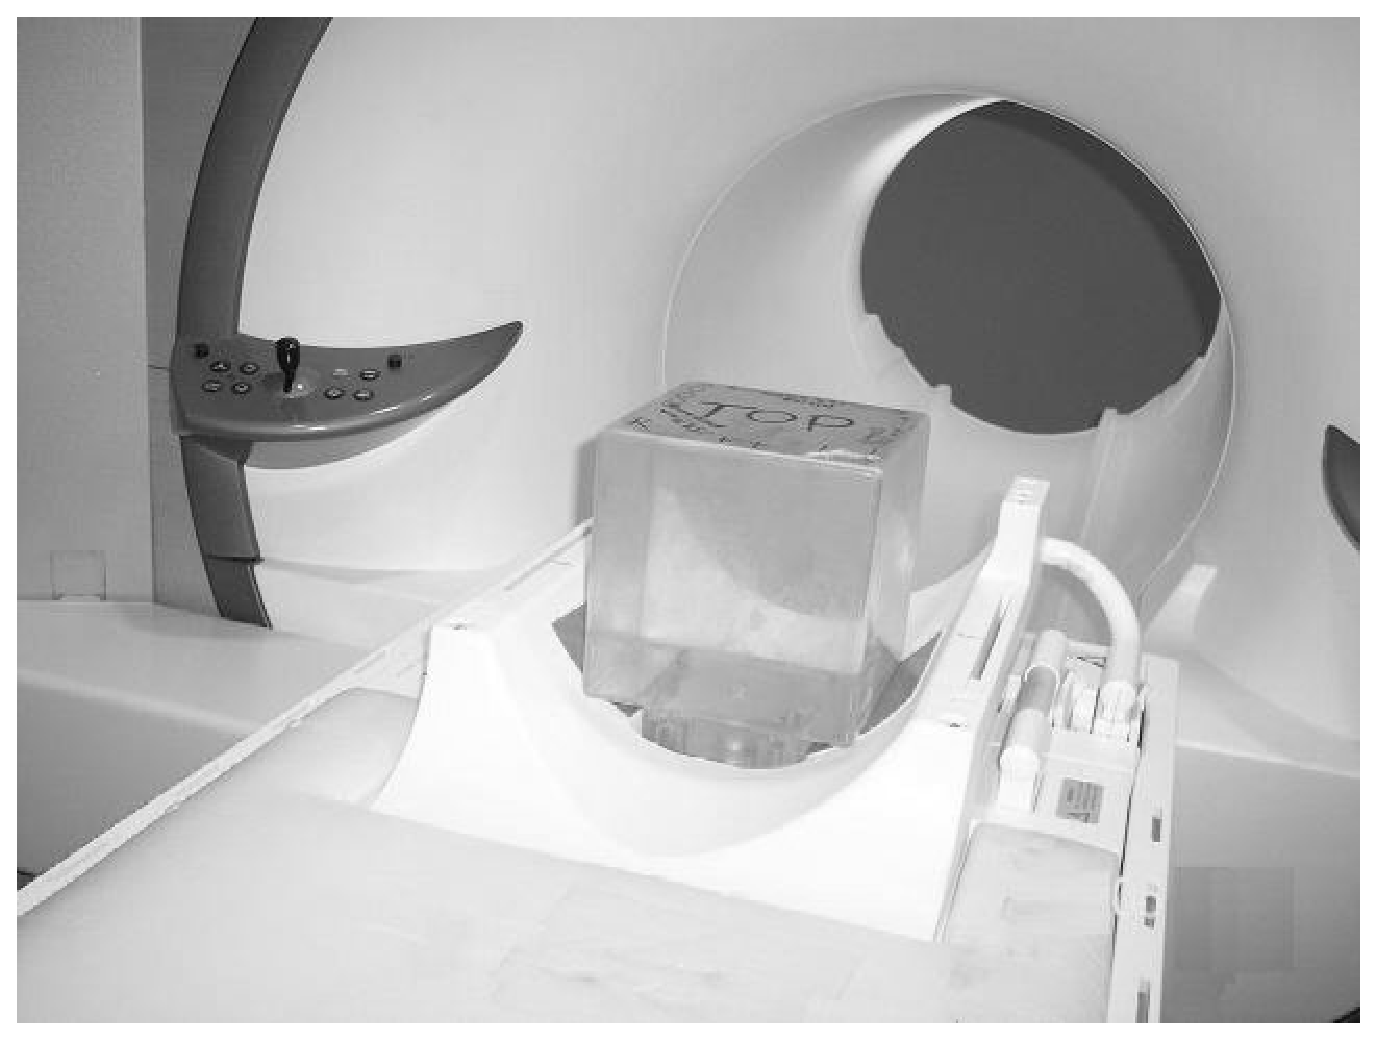
\includegraphics[width=4in]{introduction/images/phantom_scanner2.eps}}}
% %    \centerline{New device}\medskip
%     \centerline{}\medskip
%   \end{minipage}
%   \caption{A phantom cube made of plexiglas and filled with oil is ready for scanning} \label{fig:1}
% \end{figure} 

The primary purpose of this thesis was to improve the distortion correction method developed in a previous 
thesis \cite{tom}.  To do this, the following issues were addressed in this work:
\begin{itemize}
\item A new phantom was designed that can capture the distortion in modern 3-Tesla(T) MRI scanner. 
\item Algorithms were developed that can extract relevant data points from the MR images of the new phantom.
\item An new algorithm was developed that can accurately estimate the gradient isocenter of the magnetic 
  field inside 3T MRI scanners.
\item An algorithm was developed that can determine the undistortion paramters, which can then be used to 
  generate undistorted MR images.
% \item An algorithm was developed that can accurately estimate the undistortion paramters,
%   which could then be used to generate undistorted MR images.
\end{itemize}

% background 
The thesis is organized as follows. After the introduction, Chapter 2 gives background information on MRI, 
it's geometric distortion, and approaches to corrected. 
Chapter 3 describe the design details of the new phantom and several phases and changes the design 
went through. The main feature of the final design of the phantom and their importance will be discussed.
The next chapter discusses the algorithm for estimation of  gradient isocenter based on new
phantom design. % Since there is no way to know the accurate location of isocenter inside MRI scanner, not even
% the manufacture themselves, we will analyze our result using a simulate data points. 
Chapter 5 describe a series of algorithms used to extract relevant data from MR and CT images. CT images were
used in this work to obtain accurate dimensions inside the phantom.
% After isocenter algorithm we will start to discuss a series of algorithms we used to extract data points
% from MR images and CT images. CT images is used for measuring certain dimensions inside phantom due to
% limitations of manufacture's macine. 
Chapter 6 describes the procedure to estimate the parameters of the model that undistorts the distorted 
MR images. The final chapter summarizes the main results and suggests future work.
% In the final chapter, putting everything together, 
% we are using the geometric feature of the phantom and information
% obtained from MR images to estimating a undistortion parameter that can transform the distorted MR images
% back to undistorted images.

\section{Background}

The research project associated with this thesis relates to the correction of MRI images that will be used 
for functional proton radiosurgery at Loma Linda University Medical Center (LLUMC).
The clinical application of protons was first suggested over 60 years ago \cite{Wil46}.
The ability to penetrate human tissue, delivering high dosage of proton beams at a target
region and being able to concentrate on a very small target area make protons ideal for use in noninvasive 
surgery \cite{Wil46}. Currently, Loma Linda University
Medical Center (LLUMC) is using proton beams to treat patients with tumors or
vascular malformations in the brain.

Due to the effectiveness of proton radiosurgery, a new system is proposed thatl targets functional 
disorders in the brain, such as trigeminal neuralgia and Parkiinson's disease by creating small lesions in 
the brain regions affected by the disease.
% Due to the effectiveness of proton radiosurgery, a new system is proposed to treat
% even smaller targets, more specifically, cranial targets.  However, this requires higher
% accuracy of the treatment system. 
The current system can treat targets as small as 1 to 3 cm.  
Target localization is accomplished using CT and projection angiography.
% In order to achieve higher accuracy, MRI is to be used for target localization in the new system. 
MRI will to be used for target localization in the new system.
The major obstacle of using MRI is the geometric distortion on MRI images caused by the nonlinearity of the magnetic gradient fields of the scanner.
% The major obstacle of using MRI is the gradient nonlinear distortion on MRI images caused by the magnetic 
% field of the scanner.

For the proposed application, two of the most important requirements for a successful distortion 
correction are:
\begin{enumerate}
\item The distortion correction must have submillimeter accuracy.
\item The correction process must be finished within 15 minutes.
\end{enumerate}

% I added some more detail in this paragraph

%The iteracy that this work is based on presented gradient nonlinearity correction method based on a cubic phantom MRI data set\cite{tom}.

This work is based on a published method for gradient nonlinearity correction using a cubic phantom MRI data set [French article], which was also subject of a previous thesis \cite{tom}.
% This work is based on a published method for gradient nonlinearity correction using a cubic phantom MRI data set \cite{tom}. 
The published method utilizes the sum of spherical
harmonics to model the geometrically warped planes of the cube, and applies the model
to correct arbitrary image sets acquired with the same scanner. The cube is
placed in the MRI scanner such that the cube's center is exactly in the center of the MRI scanner.  This work assumes the center of the MRI scanner corresponds to the isocenter of the
magnetic field of the scanner. Opposite faces of the phantom are averaged, and three midplanes are fit to these surfaces.  Due to the symmetric property of the magnetic field,
the midplanes of different orientations of the phantom cube are undistorted.  Through each midplane, the ideal planes of different surfaces
of the cube are calculated simply by shifting the midplane to the direction
of the ideal plane by one-half the length of the cube. For each pixel on
the ideal plane, the sum of spherical
harmonics equation \ref{eq:spherical_harmonics} is applied to transform that pixel to the corresponding location on the distorted plane.

\begin{equation} \label{eq:spherical_harmonics}
\bar{\alpha} = \alpha(1 + K_{\alpha_0}(x^2 + y^2) + K_{\alpha_1}z^2 +
K_{\alpha_2}z^2(x^2 + y^2) + K_{\alpha_3}(x^2 + y^2)^2 +
K_{\alpha_4}z^4)
\end{equation}

Where $\bar{\alpha}$ and $\alpha$ are undistorted and distorted 3D coordinate respectively; $x$, $y$ and $z$ are coordinates of $\alpha$ on each axis; $K_{\alpha_i}$ are distortion parameters. Thus the distortion parameters in
equation \ref{eq:spherical_harmonics} are computed using linear least squares
technique.

Several assumptions are made for this model:
\begin{itemize}
  \item The phantom is (reasonably) centered with respect to the gradient isocenter of the scanner.
  \item The distortion is (reasonably) symmetric for each pair of faces.
  \item The origin of the DICOM patient coordinate system conincides with the position of the gradient 
    isocenter.
\end{itemize}


% However, positioning the phantom with respect to gradient isocenter is very difficult,
% making it nearly impossible to perfectly center the phantom. After performing numerous
% scans by Permedics Inc and LLUMC over the past several years, the issue of phantom centering has been 
% identified
% as a crucial factor in the quality of image data.  Improper centering of the phantom
% in the scanner produces strong asymmetry in the phantom surfaces, thereby affecting the
% accuracy of the distortion correction.  Therefore, the assumption that the distortion
% is symmetric for each pair of phantom faces is invalid.

In reality, however, these assumptions are not valid. Due to the geometry of the MR scanner, 
the phantom cannot be centered, and the phantom center will always we located in the upper half of the 
circular scanning plane. The issue of phantom centering has been identified as a crucial factor in the 
quality of distortion correction. Improper centering of the phantom in the scanner produces strong asymmetry 
in the phantom surfaces, thereby violating the asumption of symmetry of the distortion.

% The assumption that the origin of the DICOM patient coordinate system corresponds to the isocenter of the magnetic field in the MRI scanner is also invalid. Siemens
% engineers have confirmed that the true location of the gradient isocenter is unknown.
% Investigating this further appeared to confirm this claim:  every scan performed thus far features a -10mm offset in Y in order to center the field of view on the phantom.  Therefore, the DICOM origin is shifted -10mm in $Y$ for each image.  But, the distortion inherent to each pair of phantom surfaces appears to be quite symmetric.  If the gradient isocenter was truly located at the DICOM origin, then the images would be expected to contain significant asymmetry in the distortion.  This is not the case in recent phantom studies.

The assumption that the origin of the DICOM patient coordinate system corresponds to the isocenter of the magnetic field in the MRI scanner is also invalid. Siemens engineers have confirmed that the exact location of the gradient isocenter is unknown. Thus, the assumption that the origin of the DICOM patient is at the same location as the gradient isocenter will further compromise the accuracy of the distortion correction method.

% In addition, the computation, including image filtering, distortion parameters
% computation and final correction, average takes about 20-30 minutes.  In some cases, the calculation
% could require as much as 40 minutes. This is far from the ideal 15 minutes requirement for clinical use.

In addition, with the introduction of the new 3T MR scanner with a larger bore, the previous phantom, which was designed for a 1.5 T scanner with a much smaller bore, turned out to be inadequate. The new scanner had only minimal distortion in the area probed by the orginal phantom with 16 cm diameter. A larger phantom was clearly needed that also better probed the circular field of view of the scanner.

\section{Significance}

% Which equation are you referring to here?  It would be better to reference the equation, instead of saying "the equation above"

Consider the minimization of the original expression for the sum of spherical harmonics:

\begin{equation} \label{eq:spherical_harmonics_2}
0 = \alpha(1 + K_{\alpha_0}(x^2_i + y^2_i) + K_{\alpha_1}z^2_i +
K_{\alpha_2}z^2_i(x^2_i + y^2_i) + K_{\alpha_3}(x^2_i + y^2_i)^2 +
K_{\alpha_4}z^4_i)
\end{equation}

The correction method this work proposes is on a pixel-to-pixel basis instead of a plane to plane basis.
Consider a point $P$ = $[X,Y,Z]$, where $X$, $Y$, and $Z$ are represented in equation \ref{eq:spherical_harmonics_2}. Each $X$, $Y$, and $Z$ describes the distance of $P$ from the DICOM origin (gradient isocenter), previously assumed to be at [0,0,0].  Past MRI studies have confirmed that the gradient isocenter is not at [0,0,0], therefore it is necessary to shift the DICOM origin appropriately by some offset $[\delta,\beta,\gamma]$.  Shifting the DICOM origin by this amount yields the new expression for $P$:

\begin{eqnarray}
P = [X - \delta, Y - \beta, Z - \gamma]
\end{eqnarray}

Substitute the new expression for $P$ into the sum of spherical harmonics expression:

$$0 = \alpha(1 + K_{\alpha_0}((x_i - \delta)^2 + (y_i - \beta)^2)$$
$$+ K_{\alpha_1}(z_i - \gamma)^2 + K_{\alpha_2}(z_i - \gamma)^2((x_i - \delta)^2 + (y_i - \beta)^2)$$
$$+ K_{\alpha_3}((x_i - \delta)^2 + (y_i - \beta)^2)^2 + K_{\alpha_4}(z_i - \gamma)^4)$$

Therefore, by expressing $P$ in this manner, the position of the true gradient isocenter becomes
$[\delta, \beta, \gamma]$. To solve for $\delta$, $\beta$, $\gamma$ and $K_{\alpha}$, we do not need
to have a full plane, as long as enough data points exist, and each data point exhibits a significant amount of distortion. The system can be solved using a linear least squares technique.

% To collect the data sets, a new phantom (Fig \ref{fig:2}), is proposed to capture data points on only the corner sections
% of the original phantom cube.  Since these sections are located far away from the gradient isocenter, they will exhibit the largest amount
% of distortion when compared to other sections closer to the gradient isocenter. The image slices that
% would be used are those close to each surface of the phantom. For each of these images a 
% filtering process will be applied to obtain only data points on the edge of phantom cube. 

% \begin{figure}[htb]
%   \begin{minipage}{0.80\linewidth}
%     \centering
%     \centerline{\mbox{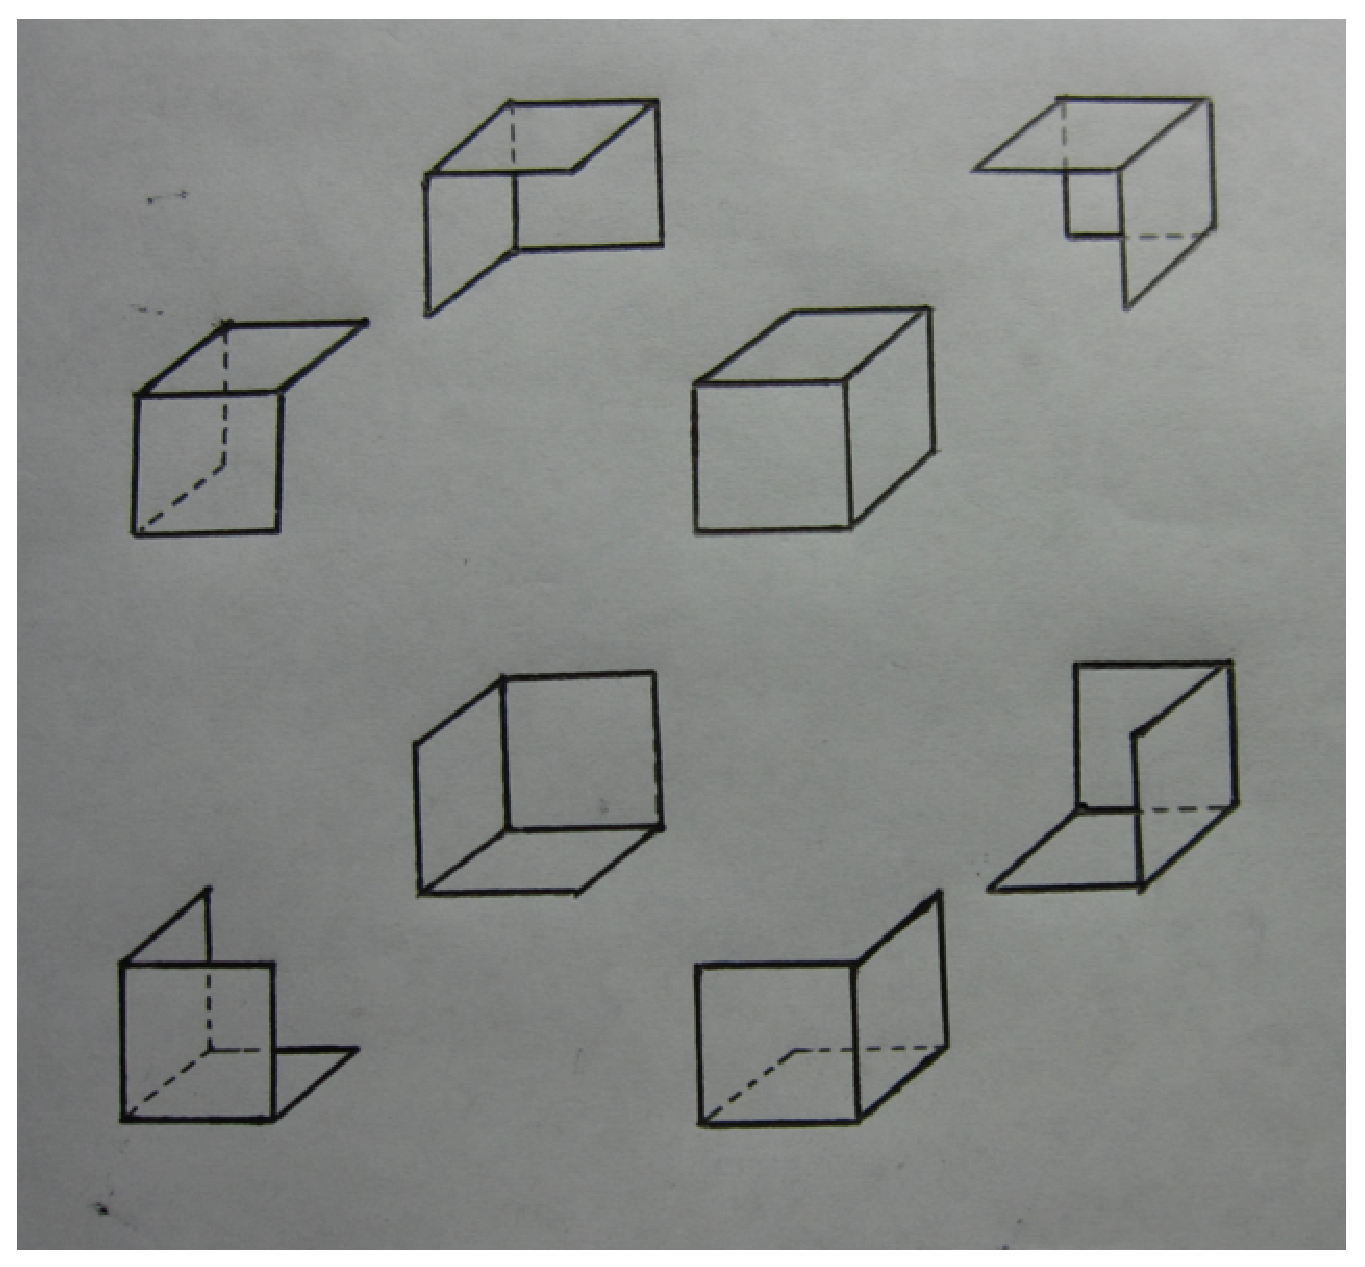
\includegraphics[width=4in]{images/model2.eps}}}
% %    \centerline{New device}\medskip
%     \centerline{}\medskip
%   \end{minipage}
%   \caption{The new phantom, designed to collect data at the corners of the MRI scan.}  \label{fig:2}
% \end{figure}

% The reason for constructing a new phantom is that a phantom cube larger than original size (159.50 mm x 159.70 mm x 158.11 mm) is needed to 
% capture the distortion of larger MRI scanner while the manufacturer who produced the original
% phantom cube was having difficulty produce an accurate cubic phantom larger than the
% one shown in \ref{fig:1}. The eight parts, shown in fig \ref{fig:2}, will be interconnected and placed inside a water tank for scanning.
% For each image, eight curves representing the intersection between the surface of the material
% and water will be obtained, and will be used for calculating the gradient nonlinearity distortion correction.


\Chapter{Background}
\label{background}

% \Chapter{Overview}
% \label{overview}
% \input{overview/main}

% algorithm overviews
% canny, peakdet, steepest descent, dicom coordinate conversion etc

\Chapter{Phantom Design}
\label{phantom_design}
\section{Introduction}

Magnetic Resonance Imaging (MRI) provides an excellent modality for distinguishing different tissues in the
human body, which is essential for medical applications. When MRI is used for stereotactic treatment planning,
its geometric accuracy is crucial. Previous studies have been conducted to correct the distortion caused by
nonlinearity of the MRI scanner’s magnetic gradient fields by imaging a cubic phantom \cite{Lang99},
\cite{LSS08b} and defining
distortion correction functions based on the distorted appearance its surfaces. Correct mathematical handling
of the distortion correction function required that the cube was centered about the magnetic isocenter, which
is defined as the common center of the three magnetic gradient fields and  is not very accurately known.
New 3Tesla MRI systems have a larger bore, making the previous phantom design impractically small for probing
the field nonlinearity in the periphery of the bore, as the phantom cannot be scaled up due to constraints
related to weight and cost of manufacturing. We are introducing a new phantom design using a different
approach, which can be built to a larger size, improves accuracy of distortion characterization and reduces
cost.

\section{Initial Design}

The original phantom design, a 16-cm oil-filled cube, could not be scaled up due to weight and manufacturing
constraints. Our first modification was to look at changing the material to FR-4 since it is rigid, very flat,
and could be submerged for short periods of time to permit scanning the solid liquid interface in an MRI
machine.  Since most of the distortion is visible only in the corners, this was rapidly replaced by 8 corners
of a virtual cube, which could be connected by a rigid frame.  The weight of a tank to submerge either of
these designs to allow scanning was prohibitive, requiring a complete redesign.

\begin{figure}[htb]
  \begin{minipage}[t]{2.75in}
    \centering
    \centerline{\mbox{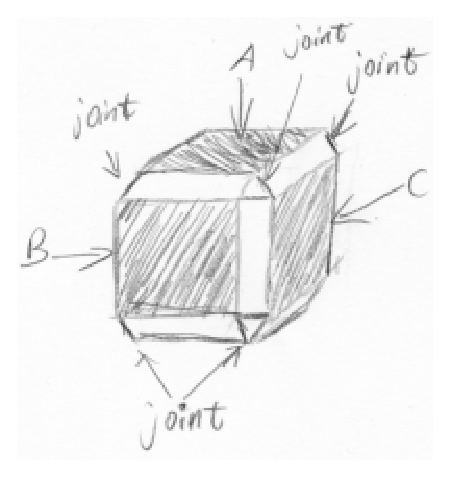
\includegraphics[width=2.75in]{phantom/images/brain_storm/model1.eps}}}
    \centerline{\emph{(a) First model}}
  \end{minipage}\medskip
  \begin{minipage}[t]{2.75in}
    \centering
    \centerline{\mbox{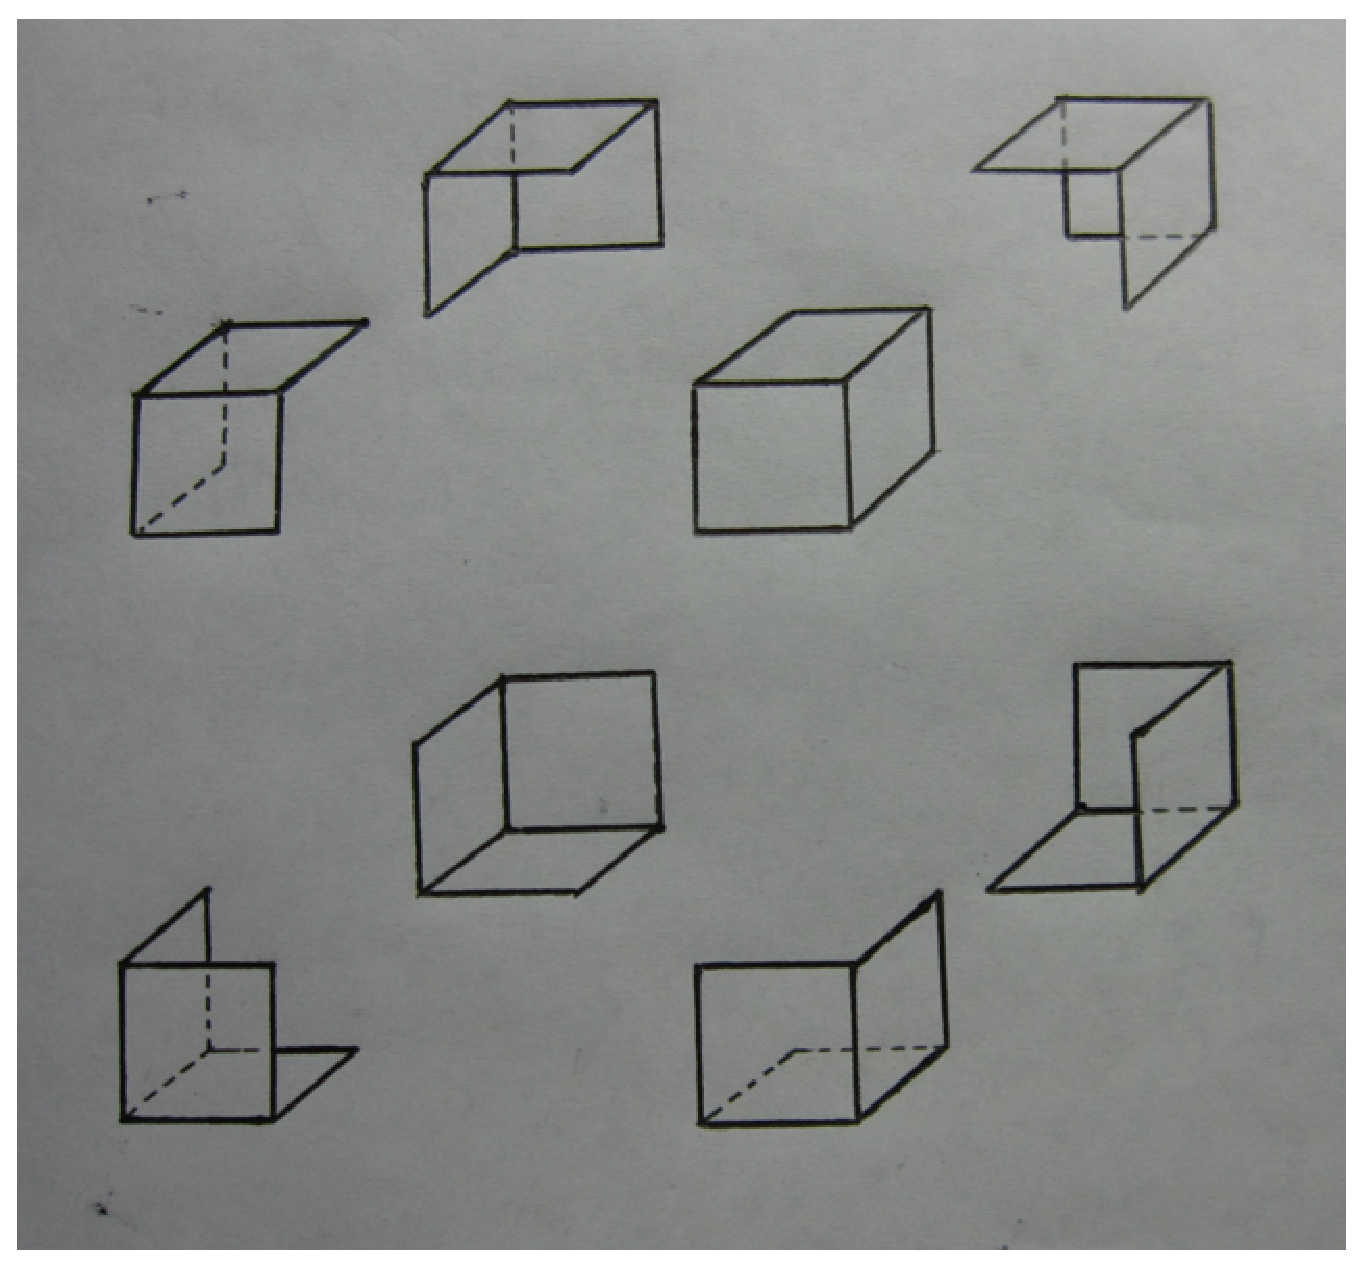
\includegraphics[width=2.75in]{phantom/images/brain_storm/model2.eps}}}
    \centerline{\emph{(b) Second model}}
  \end{minipage}
\end{figure}


\section{New Design}

The phantom is shaped to be as large as possible, while still fitting in the head coil of the scanner, so as
to achieve the maximum quality of signal and largest distortion. The phantom is an octagonal prism with 205mm
between opposite sides.  Each face of the octagonal prism is composed of 8 high precision NMR tubes that are
5mm in outer diameter and 205 mm in length. These tubes are filled with copper sulfate solution to generate a
strong signal in an MRI scanner.  The tubes are placed parallel to the magnetic field so they will cause less
susceptibility distortion \cite{mag_susceptibility},
and thus provide more accurate information on the gradient field.  In the
center of the phantom is a large water tank to help intensify the signals generated by the tubes. At one end
of the phantom is a cylindrical tank filled with copper sulfate, with a number of small solid cylinders in a
hexagonal pattern that are connecting the two surfaces of the tank. These cylinders are used to maintain the
long-term accuracy of the two surfaces, making sure they won’t deform, and are also aligned to the field to
minimize their effect on the field.  The data generated from 64 tubes mounted on the sides are designed to
give us x and y axis distortion information, and the end tank is designed to provide z-axis distortion data,
allowing a complete 3-D distortion correction with a relatively small amount of data.

\section{Sealing NMR Tubes}

Our original idea for sealing the NMR tubes was to use paraffin wax, either with or without a silicon seal.
Paraffin was heated and a liquid drop was then added to the tube as a seal , but had an uneven bottom caused
by the rapid solidifying of the wax, when it came in contact with the copper sulfate.  Additionally,
it tended to trap air bubbles, which made the end very hard to work with in the images.  Worst yet, after a
few weeks the liquid level in the tubes started to drop.  We decided to compare three potential alternatives:
machinable wax, water weld, and silicon sealer.  As the images on the right show, the silicon was far and
away the best.  There was no leakage lost, and since the setup time was slower on the liquid side it ended
up being almost completely flat.  Every feature was met, and it was also the most cost effective solution.

\begin{figure}[htb]
  \begin{minipage}[t]{1in}
    \centering
    \centerline{\mbox{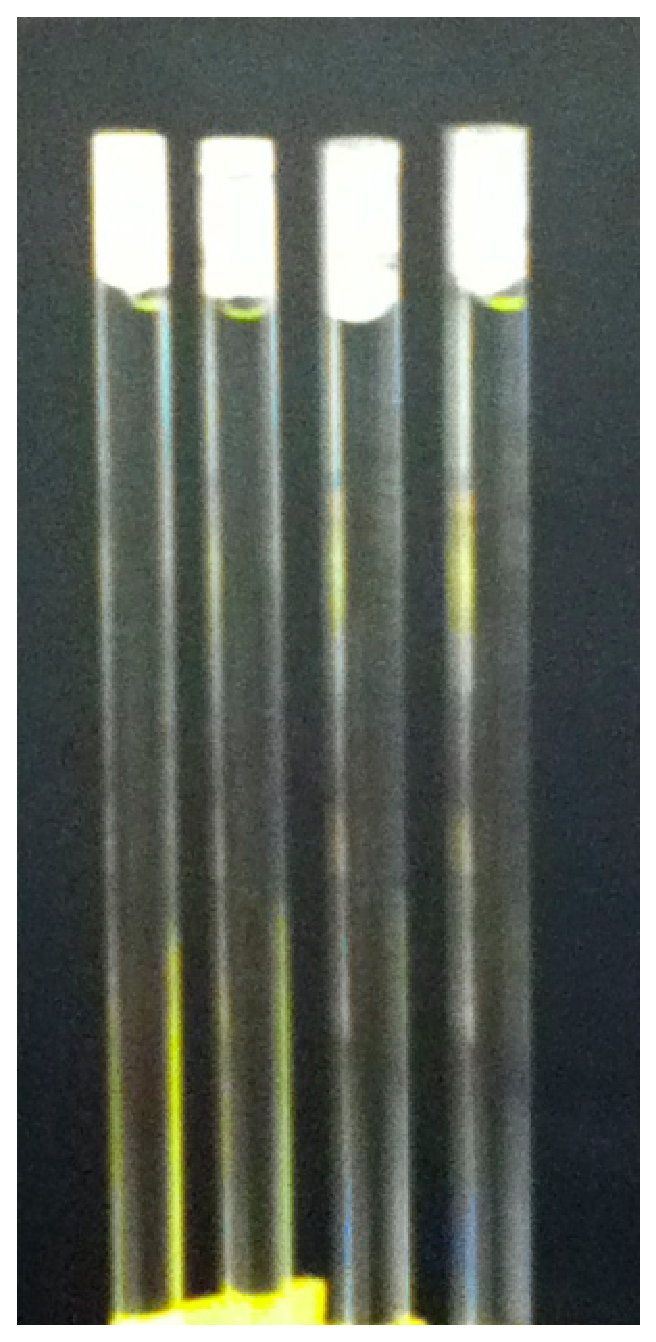
\includegraphics[width=1in]{phantom/images/tube_sealings/paraffin_and_floable_silicon.eps}}}
    \centerline{\emph{(a) Paraffin wax at top with floatable silicon at bottom}}
  \end{minipage}
  \begin{minipage}[t]{1in}
    \centering
    \centerline{\mbox{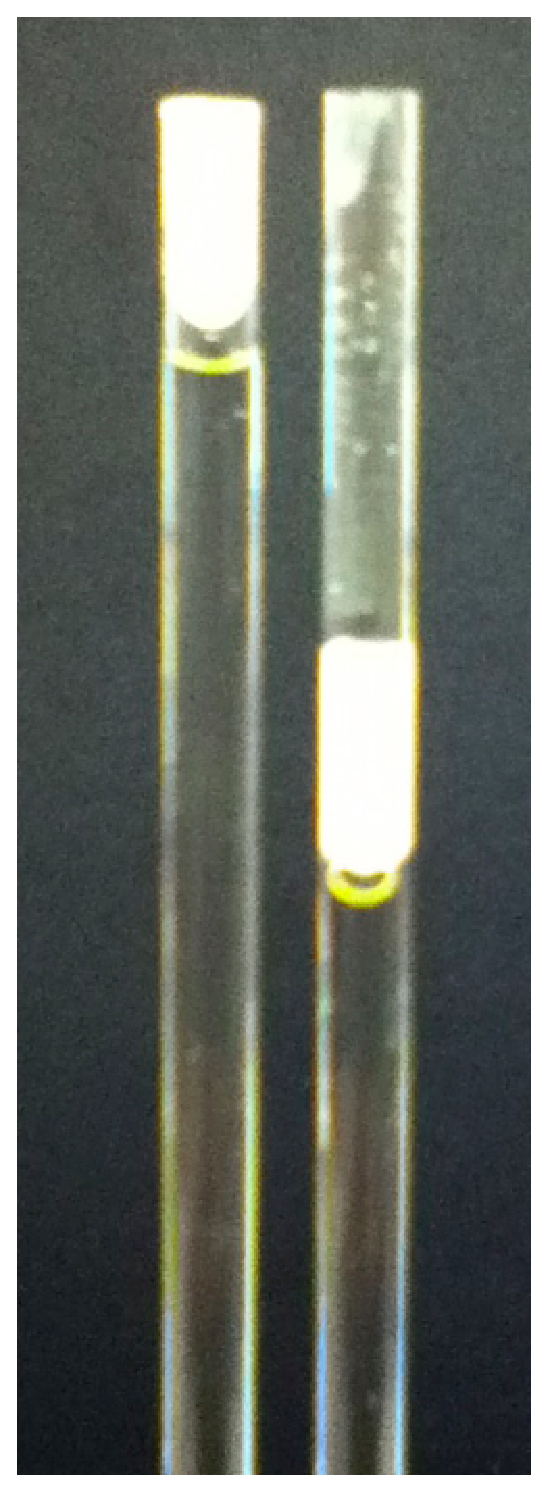
\includegraphics[width=1in]{phantom/images/tube_sealings/paraffin.eps}}}
    \centerline{\emph{(b) Paraffin wax only}}
  \end{minipage}

  \begin{minipage}[t]{1in}
    \centering
    \centerline{\mbox{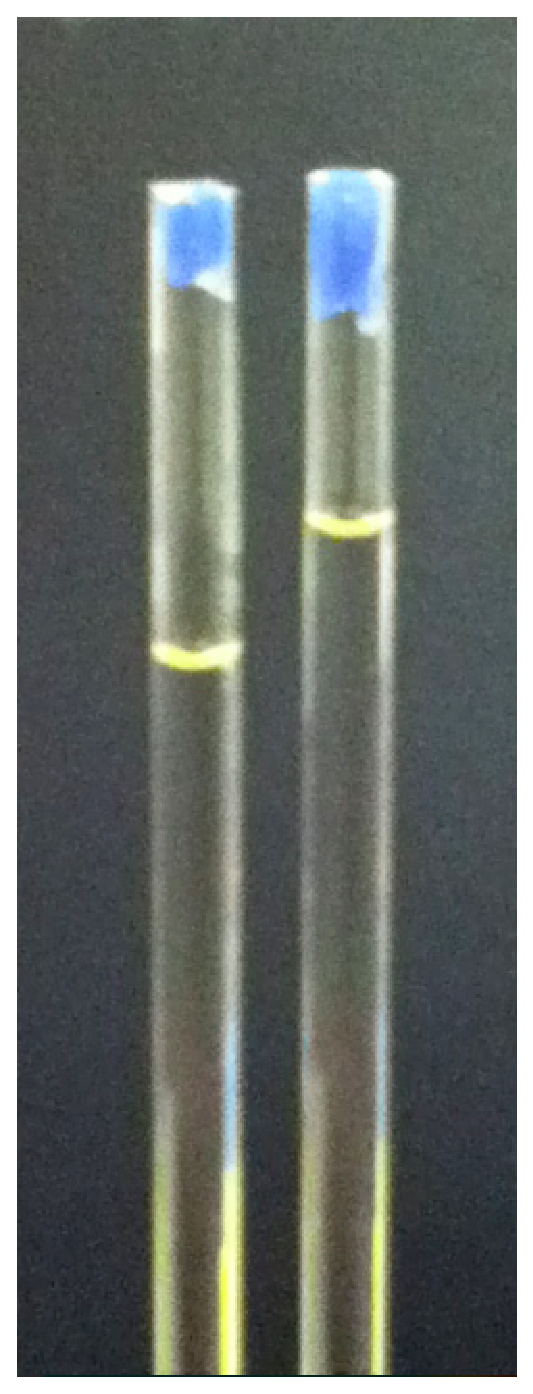
\includegraphics[width=1in]{phantom/images/tube_sealings/machinable_wax.eps}}}
    \centerline{\emph{(c) Machinable wax}}
  \end{minipage}\medskip
  \begin{minipage}[t]{1in}
    \centering
    \centerline{\mbox{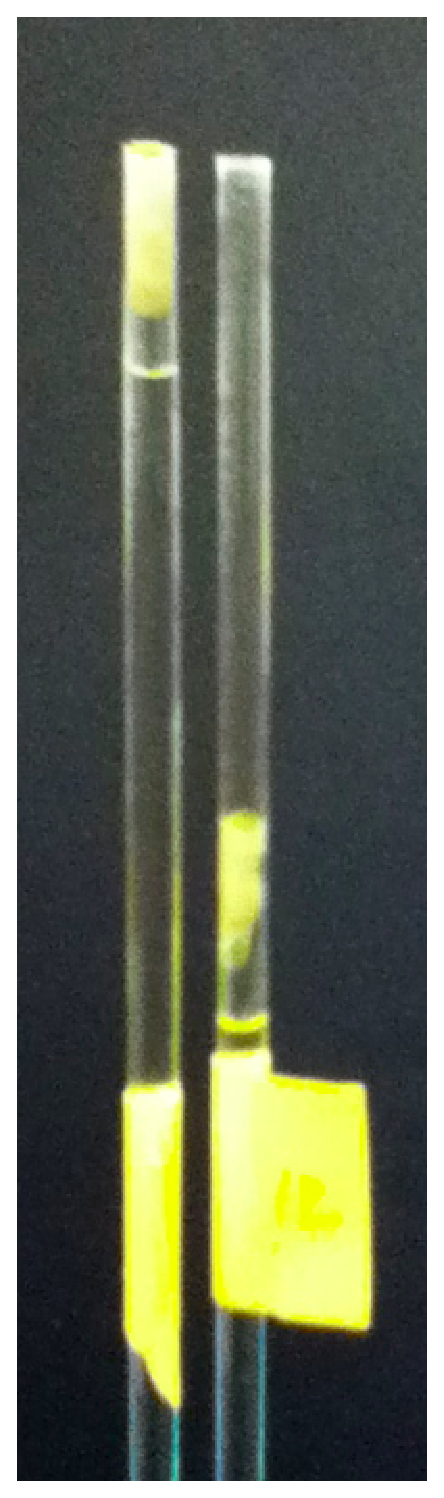
\includegraphics[width=1in]{phantom/images/tube_sealings/water_weld.eps}}}
    \centerline{\emph{(d) Water weld}}
  \end{minipage}

  \begin{minipage}[t]{1in}
    \centering
    \centerline{\mbox{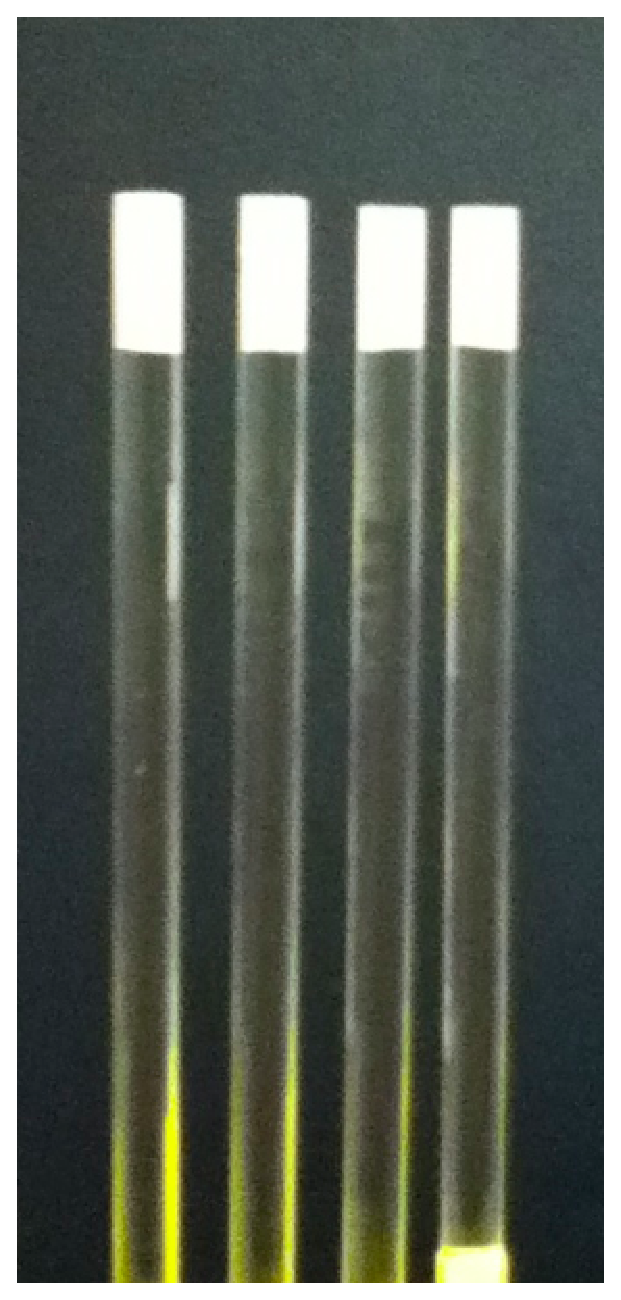
\includegraphics[width=1in]{phantom/images/tube_sealings/silicon.eps}}}
    \centerline{\emph{(e) Silicon}}
  \end{minipage}

\end{figure}

\section{Updated Desgin}

% \begin{figure}[htb]
%   \begin{minipage}[t]{1in}
%     \centering
%     \centerline{\mbox{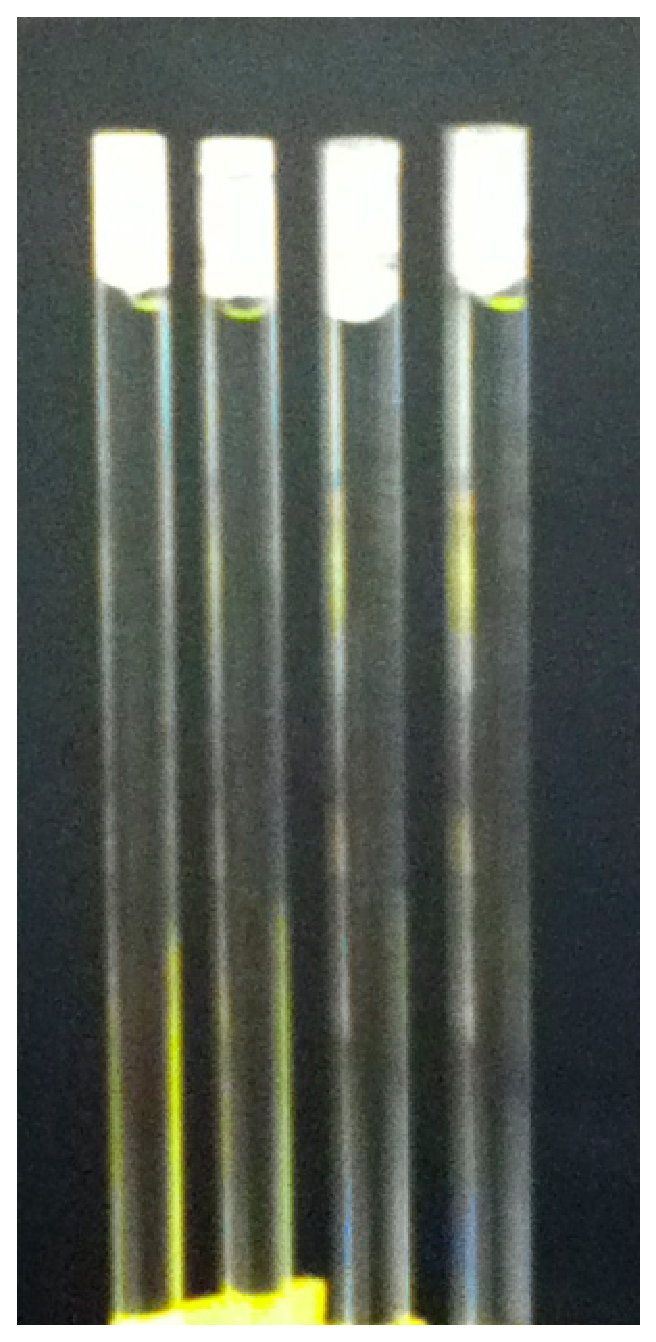
\includegraphics[width=1in]{phantom/images/tube_sealings/paraffin_and_floable_silicon.eps}}}
%     \centerline{\emph{(a) Paraffin wax at top with floatable silicon at bottom}}
%   \end{minipage}
%   \begin{minipage}[t]{1in}
%     \centering
%     \centerline{\mbox{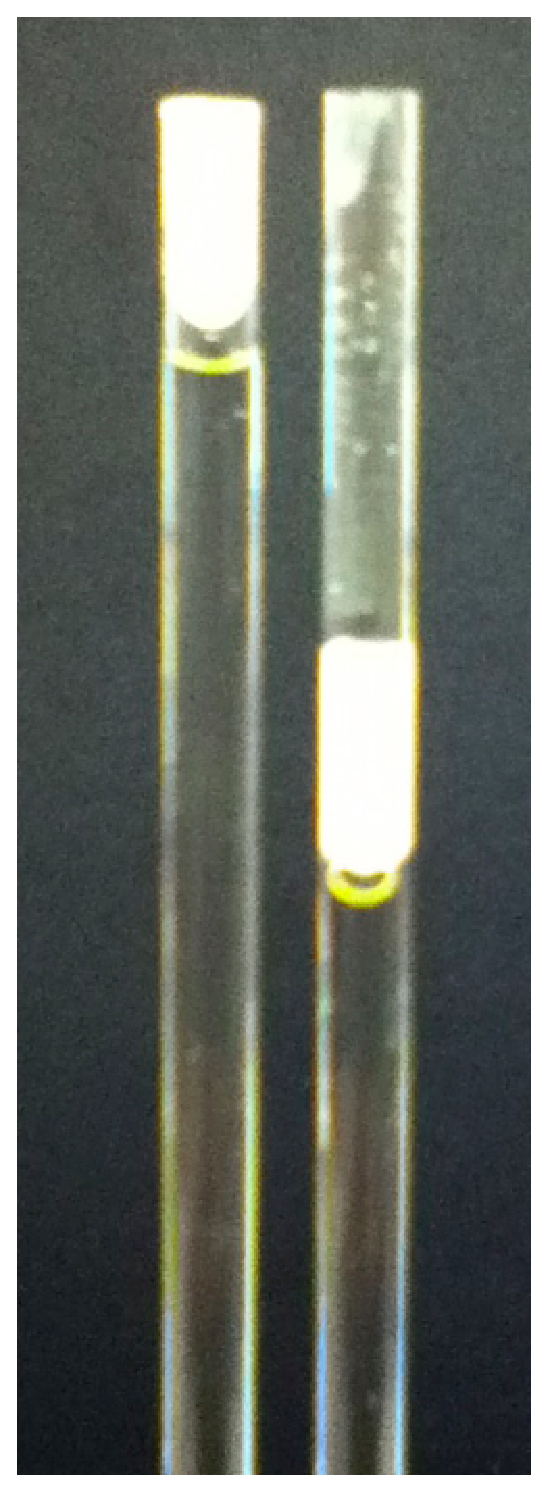
\includegraphics[width=1in]{phantom/images/tube_sealings/paraffin.eps}}}
%     \centerline{\emph{(b) Paraffin wax only}}
%   \end{minipage}

%   \begin{minipage}[t]{1in}
%     \centering
%     \centerline{\mbox{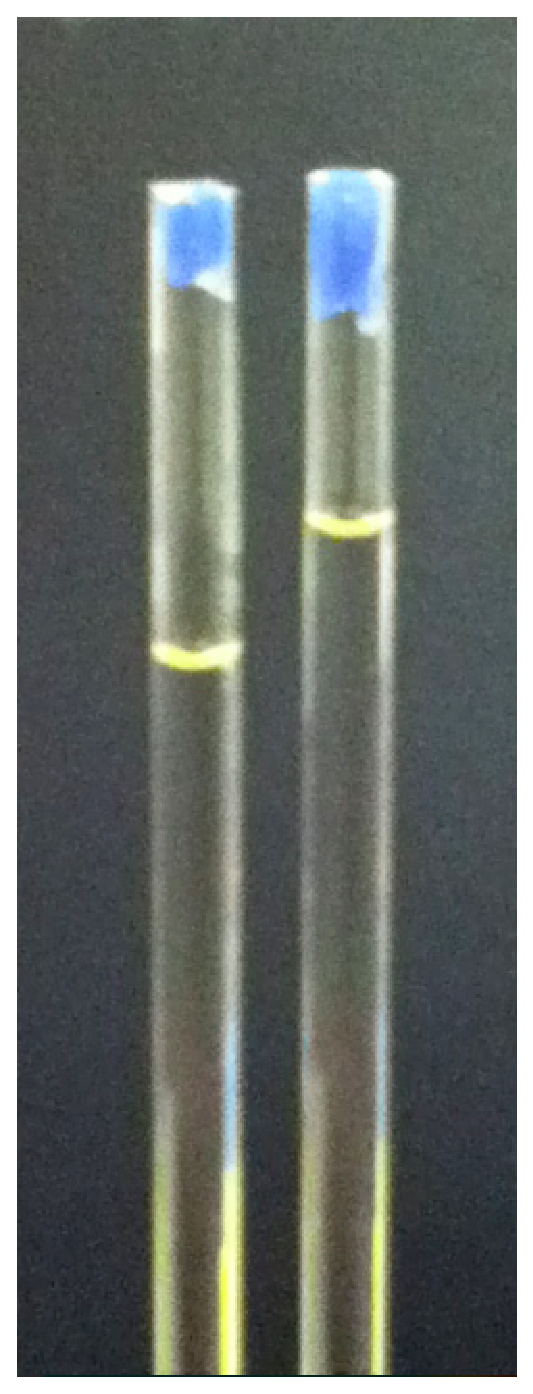
\includegraphics[width=1in]{phantom/images/tube_sealings/machinable_wax.eps}}}
%     \centerline{\emph{(c) Machinable wax}}
%   \end{minipage}\medskip
%   \begin{minipage}[t]{1in}
%     \centering
%     \centerline{\mbox{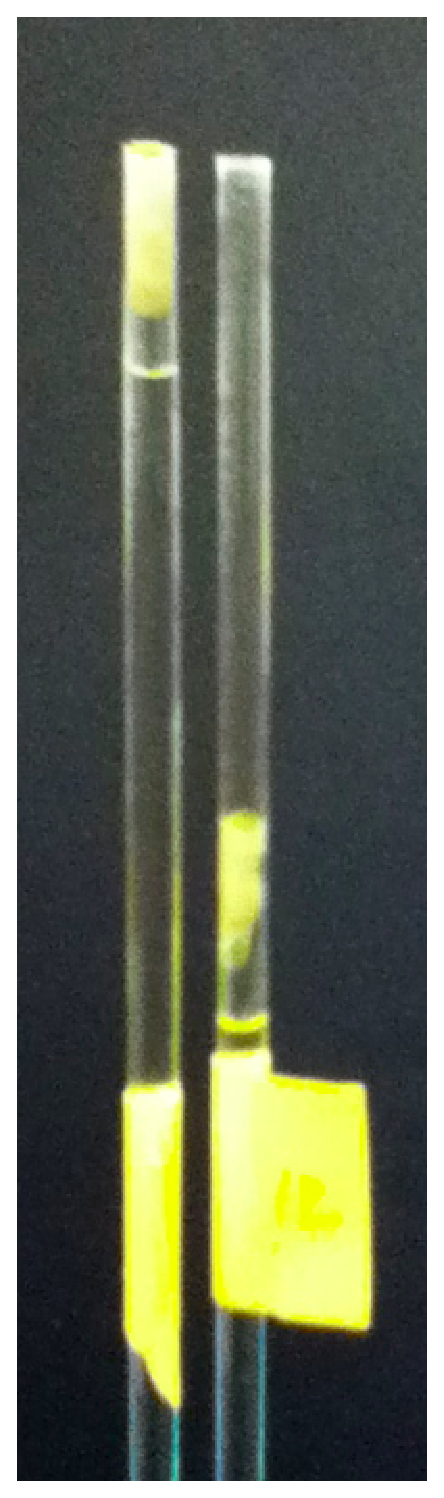
\includegraphics[width=1in]{phantom/images/tube_sealings/water_weld.eps}}}
%     \centerline{\emph{(d) Water weld}}
%   \end{minipage}

%   \begin{minipage}[t]{1in}
%     \centering
%     \centerline{\mbox{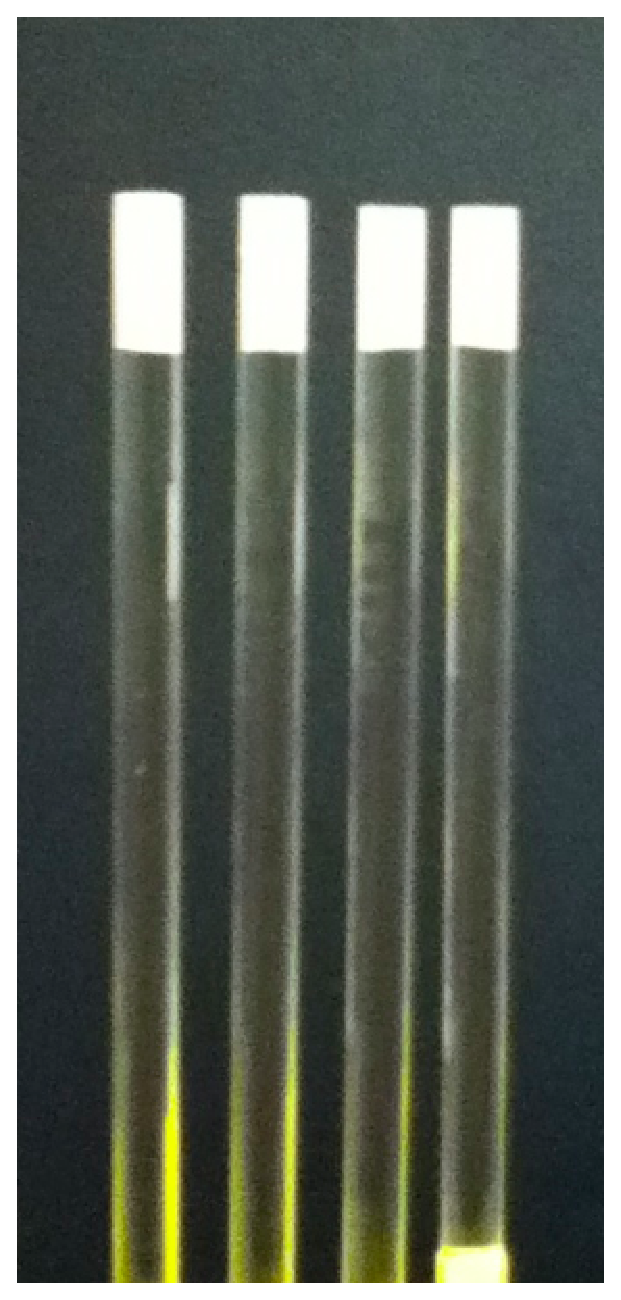
\includegraphics[width=1in]{phantom/images/tube_sealings/silicon.eps}}}
%     \centerline{\emph{(e) Silicon}}
%   \end{minipage}

% \end{figure}


\section{Installation and Use}

The new phantom is designed to rest in the head coil of a 3T MRI scanner.  It has a back plate with several
leveling screws to align the phantom in the head coil using the laser alignment system.  This alignment is
aided by alignment marks on the outside of the phantom. The phantom is then moved into the MRI scanner,
and its center is placed as close to the isocenter as possible.  While it is not required to be centered,
centering does improve the performance.  A quick alignment scan is used to ensure the phantom is in the best
location possible.  When this is done the scan is taken and processed using distortion detection and
correction software, which is not subject of the present presentation.

\section{Initial Experience}

The original phantom design, a 16-cm oil-filled cube, could not be scaled up due to weight and manufacturing
constraints. Our first modification was to look at changing the material to FR-4 since it is rigid, very flat,
and could be submerged for short periods of time to permit scanning the solid liquid interface in an MRI
machine.  Since most of the distortion is visible only in the corners, this was rapidly replaced by 8 corners
of a virtual cube, which could be connected by a rigid frame.  The weight of a tank to submerge either of
these designs to allow scanning was prohibitive, requiring a complete redesign.

\section{Conclusion}

A new phantom for the measurement and correction of nonlinear gradient field distortion of MRI systems is
presented.  It is lighter, more economic, and allows for both more accurate measurement of field distortion
and the location of the isocenter. 

\Chapter{Gradient Isocenter Localization}
\label{iso_center}
\subsection{Introduction}
\label{Introduction}
%The isocenter of the magnetic gradient fields inside a Magnetic Resonance (MR) Imaging scanner is used in many distortion correction methods for MR images~\cite{Dor05,LSS06a,LSS06b,LSS08a,LSS08b,Lang99,Wang04a,Wang04b}.  Currently there is no known method for estimating the gradient isocenter. All existing estimation methods are using the DICOM patient center which is very close but not exactly the same as isocenter. The different between isocenter and DICOM patient center could contribute part of the error of overall correctness of estimation.

Magnetic resonance imaging (MRI) provides an excellent modality for distinguishing different tissues in the human body, which makes this modality essential for medical applications. MRI can also be used for treatment planning of medical procedures that require a great degree of geometrical accuracy such as  functional radiosurgery~\cite{Kond99}. Unfortunately, the accuracy of MRI for medical targeting applications is compromised by the presence of geometric distortions such as non-linearities of the magnetic gradient fields or inhomogeneities of the scanner main field ~\cite{Dor05,LSS06a,LSS06b,LSS08a,LSS08b,Lang99,Wang04a,Wang04b}. Gradient nonlinearities can cause over 2mm of distortion to the location of features in the image~\cite{LSS08b,Lang99}.

Modern MRI scanners have built-in distortion correction algorithms, that rely on knowledge of the magnetic field configuration and its distortion. Built-in algorithms, which are usually proprietary, are designed based on assumed knowledge of the geometry and location of the gradient coils. A more practical approach is to use a phantom of known geometry and to derive the distortion by analyzing the MRI images generated with such a phantom ~\cite{Dor05,LSS06a,LSS06b,LSS08a,LSS08b,Lang99,Wang04a,Wang04b}. This method has the advantage that a scanner-specific correction can be applied, which can also take into account potential changes in the gradient fields over time.

Accurate knowledge of the gradient isocenter is essential to very accurate distortion correction methods, To our knowledge, existing distortion correction algorithms, both built-in and phantom based, make the assumption that the gradient isocenter coincides with the origin of the DICOM coordinates. This assumption may not be accurate and should not be used if a high degree of accuracy is necessary.

The goal of this work was to develop and implement a numerical software-based method to estimate the gradient isocenter of the magnetic field inside an MRI scanner using the MRI scan of a custom-built phantom.  In our previous work~\cite{LSS06a,LSS06b,LSS08a,LSS08b}, we used an oil filled plexiglas cube with
159.50mm $\times$ 159.70mm $\times$ 158.11mm dimension that was designed to fit MR scanners that were available at that time.  Current MRI scanners have a significantly wider aperture, which necessitates a larger phantom to characterize the field distortion.  Furthermore, since the lower part of the scanner aperture is occupied by the scanner table, the scanning area occupied by the phantom or the patient is not centered on the gradient isocenter, making correction methods that assume that the phantom is centered with respect to the gradient isocenter~\cite{LSS06a,LSS06b,LSS08a,LSS08b,Lang99} obsolete and potentially inaccurate.

\subsection{Distortion Phantom}
A new phantom design was developed with the intention to probe the distortion in the 50 cm field-of-view (FOV) of a modern 3T MRI scanner (Magnetom Trio, Siemens).  Due to the geometry of the gradient field nonlinearity, the distortion is largest in the outer fringes of the FOV~\cite{LSS06a,LSS06b,LSS08a,LSS08b}. Capturing distortion data in the periphery of the FOV is important for better accuracy of the distortion correction. Building a very large cubical oil-filled phantom is a challenge due to weight limitations and limited capability to accurately machine a very large flat surface. Thus it was felt to be impractical to simply scale up the original phantom.  Another limitation is that the phantom needs to fit inside the scanner head coil which needs to be used to achieve a sufficiently high signal-to-noise ratio.  To meet all requirements, we designed a phantom that is comprised of 64 NMR glass tubes of 3 mm inner diameter, filled with copper sulfate and arranged in 8 surfaces forming an octagon.  A water-filled cylinder in the middle of the octagon ensures a good signal generated by the tubes.  The distance between tubes on the opposite side of the surface is 205mm, which is about 28\% wider than the original phantom. In addition we also added four more surfaces to provide data and better fit the headcoil.  There are 8 removable tubes on each surface with 10 mm gap between adjacent tubes.  Each tube is about 207 mm long, which is also an increase of about 28\% in length from the original phantom.  Tubes are placed along the main axis of the magnetic $B_0$  field to reduce the effects of chemical shift and magnetic susceptibility and
resulting in high-quality axial images.

\subsection{Computational Algorithm}

The algorithm we described here is using simulated data set that is based the
geometric property of the phantom and the properties of the MR images.
The MR images we are using have 1mm per pixel resolution for every image and
1mm thickness between two adjacent planes. In the simulation, we will be using millimeters as unit for
each data point. Since the images we are using to collect data points are all axial scans,
we will only add noise to x and y coordinate of each data point.

\subsection{Tube Modeling}

The tubes is 203 mm long. So our simulation data is ranging from -100 to 100 on z axis for each tube.
The arrangement of the tubes could be seen in Figure~\ref{fig:1}.
Our algorithm is based on two standard assumptions~\cite{LSS06a,LSS06b,LSS08a,LSS08b,Lang99}.: (1) the distortion in MR images are only caused by the magnetic field inside MRI scanner and (2) the magnetic field can be perfectly described using the sum of spherical harmonic.

\begin{figure}[htb]

  \begin{minipage}[b]{1.65in}
    \centering
    \centerline{\mbox{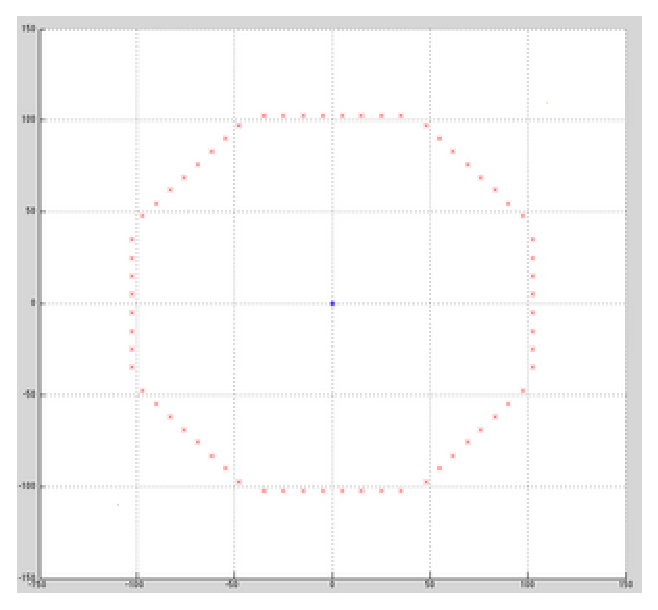
\includegraphics[width=1.65in]{isocenter/images/simulation/axial_no_distortion.eps}}}
    \centerline{\emph{(a) Axial view.}}\medskip
  \end{minipage}
  \hfill
  \begin{minipage}[b]{1.65in}
    \centering
    \centerline{\mbox{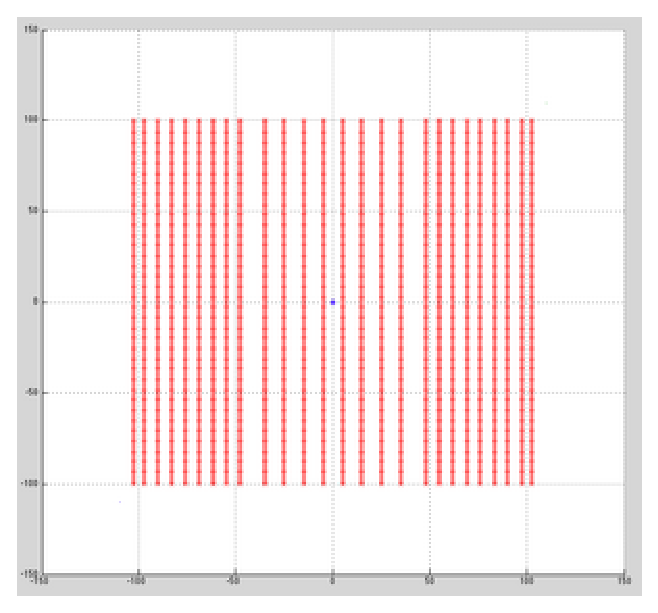
\includegraphics[width=1.65in]{isocenter/images/simulation/coronal_no_distortion.eps}}}
    \centerline{\emph{(b) Coronal view.}}\medskip
  \end{minipage}
%\hfill
%
\caption{\emph{Phantom modeling without distortion}} \label{fig:1}
%
\end{figure}

The spacial coordinate of the phantom must be transformed into a coordinate relative to the gradient isocenter
of the magnetic field, see Equation~\ref{eq1}, then using the first 5 terms of the spherical harmonic we can estimate
a offset in $x$, $y$, $z$ direction, see Equation~\ref{eq2}. Finally this offset is added the original coordinate
to create a distorted model, see Equation~\ref{eq3}.  Also a very key requirement for this algorithm is that the z-axis the phantom which is parallel to the tubes must be aligned with the z-axis of the magnetic field.

\begin{eqnarray}
\begin{bmatrix}
x^\prime  \\
y^\prime  \\
z^\prime  \\
\end{bmatrix}
& = &
\begin{bmatrix}
x \\
y \\
z \\
\end{bmatrix}
-
\begin{bmatrix}
x_{iso} \\
y_{iso} \\
z_{iso}\\
\end{bmatrix}
\label{eq1}
\\
K & = &
\begin{bmatrix}
K_{x_0} \; K_{x_1} \; K_{x_2} \; K_{x_3} \; K_{x_4} \\
K_{y_0} \; K_{y_1} \; K_{y_2} \; K_{y_3} \; K_{y_4} \\
K_{z_0} \; K_{z_1} \; K_{z_2} \; K_{z_3} \; K_{z_4} \\
\end{bmatrix}
\\
\begin{bmatrix}
\alpha \\
\beta \\
\zeta \\
\end{bmatrix}
& = &
K
\begin{bmatrix}
{x^\prime}^2 + {y^\prime}^2 \\
{z^\prime}^2 \\
{z^\prime}^2 {({x^\prime}^2 + {y^\prime}^2)}^2 \\
{({x^\prime}^2 + {y^\prime}^2)}^2 \\
{z^\prime}^4 \\
\end{bmatrix}
\end{eqnarray}
\begin{eqnarray}
\begin{bmatrix}
  \Delta x \\
  \Delta y \\
  \Delta z \\
\end{bmatrix}
& = &
\begin{bmatrix}
x^\prime \alpha \\
y^\prime \beta \\
z^\prime \zeta \\
\end{bmatrix}
\label{eq2}
\\
\begin{bmatrix}
\bar{x} \\
\bar{y} \\
\bar{z} \\
\end{bmatrix}
& = &
\begin{bmatrix}
x + \Delta x \\
y + \Delta y \\
z + \Delta z \\
\end{bmatrix}
\label{eq3}
  % \bar{\alpha_i} & = & \alpha_i \left(1+  K_{\alpha_0} \left((x_i - ISO_x)^2 + (y_i - ISO_y)^2 \right)  \right. \nonumber\\
  % &&\qquad      \left.    + K_{\alpha_1}(z_i - ISO_z)^2 \right. \nonumber\\
  % &&\qquad      \left.    + K_{\alpha_2}(z_i - ISO_z)^2 \left((x_i - ISO_x)^2 + (y_i - ISO_y)^2 \right)  \right. \nonumber\\
  % &&\qquad      \left.    + K_{\alpha_3} \left((x_i - ISO_x)^2 + (y_i - ISO_y)^2 \right)^2 \right. \nonumber\\
  % &&\qquad      \left.    + K_{\alpha_4}(z_i - ISO_z)^4 \right)
% \label{eq6}
\end{eqnarray}

\subsection{ISO-Center Coordinate Estimation}

Using a exaggerated distortion parameter we can visualize the shape of the distortion model. Without distortion, the phantom appears as in Figure~\ref{fig:1}.  With large distortions, the phantom appears as in Figure~\ref{fig:2}, which is useful to understand the form of the distortions.  A more realistic distortion can be seen in Figure~\ref{fig:3}, which uses distortion parameters from~\cite{LSS08b}.


\begin{figure}[htb]

  \begin{minipage}[b]{1.65in}
    \centering
    \centerline{\mbox{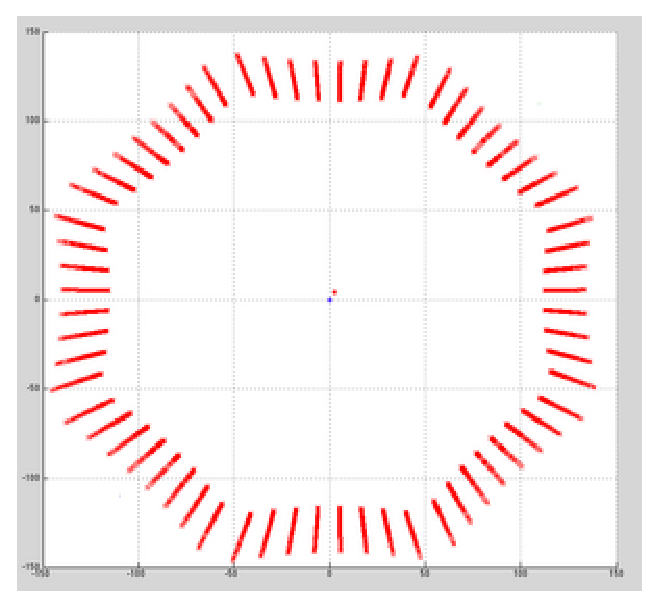
\includegraphics[width=1.65in]{isocenter/images/simulation/axial_distortion_0.eps}}}
    \centerline{\emph{(a) Axial view.}}\medskip
  \end{minipage}
  \hfill
  \begin{minipage}[b]{1.65in}
    \centering
    \centerline{\mbox{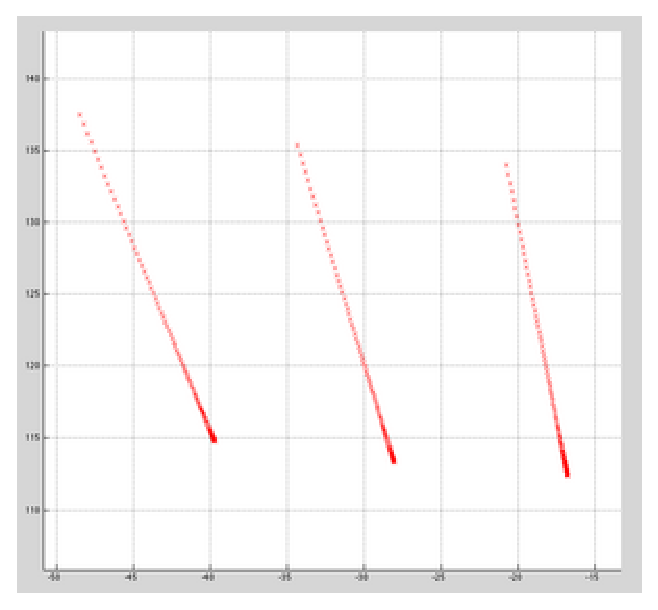
\includegraphics[width=1.65in]{isocenter/images/simulation/axial_tube_distortion_0.eps}}}
    \centerline{\emph{(b) Enlarged axial view.}}\medskip
  \end{minipage}
  \begin{minipage}[b]{1.65in}
    \centering
    \centerline{\mbox{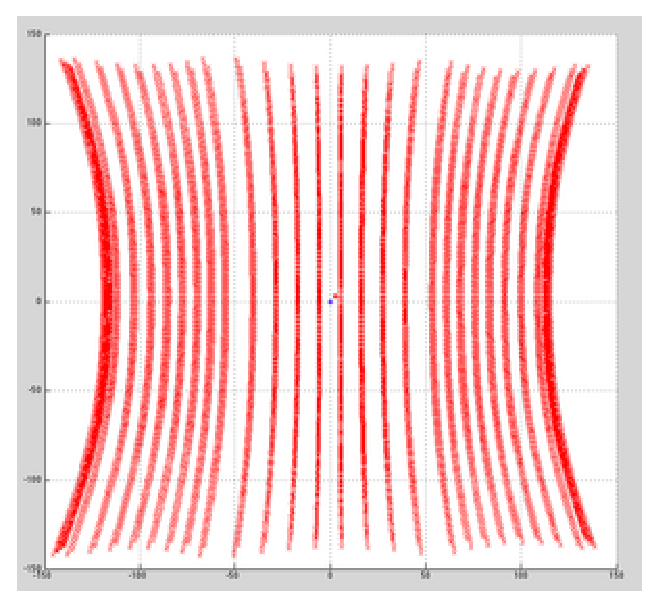
\includegraphics[width=1.65in]{isocenter/images/simulation/coronal_distortion_0.eps}}}
    \centerline{\emph{(c) Coronal view.}}\medskip
  \end{minipage}
%\hfill
%
\caption{\emph{Phantom modeling with large distortions}} \label{fig:2}
%
\end{figure}

\begin{figure}[htb]

  \begin{minipage}[b]{0.48\linewidth}
    \centering
    \centerline{\mbox{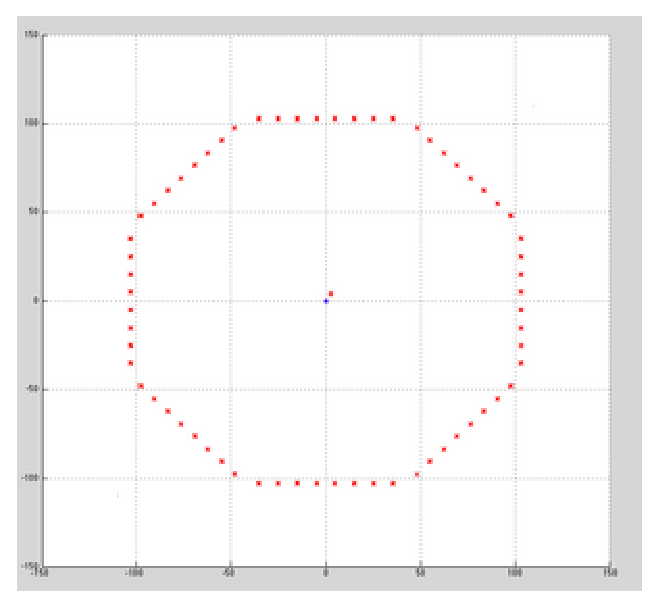
\includegraphics[width=1.65in]{isocenter/images/simulation/axial_distortion_1.eps}}}
    \centerline{\emph{(a) Axial view.}}\medskip
  \end{minipage}
  \hfill
  \begin{minipage}[b]{0.48\linewidth}
    \centering
    \centerline{\mbox{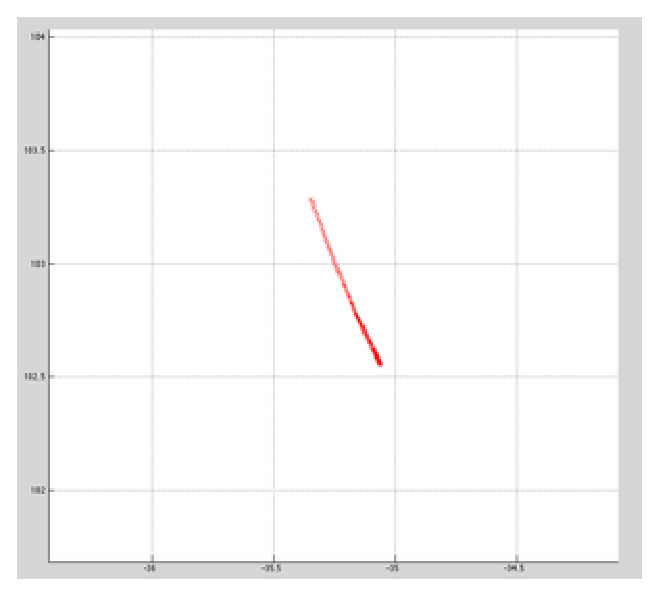
\includegraphics[width=1.65in]{isocenter/images/simulation/axial_tube_distortion_1.eps}}}
    \centerline{\emph{(b) Enlarged axial view.}}\medskip
  \end{minipage}
  \begin{minipage}[b]{0.48\linewidth}
    \centering
    \centerline{\mbox{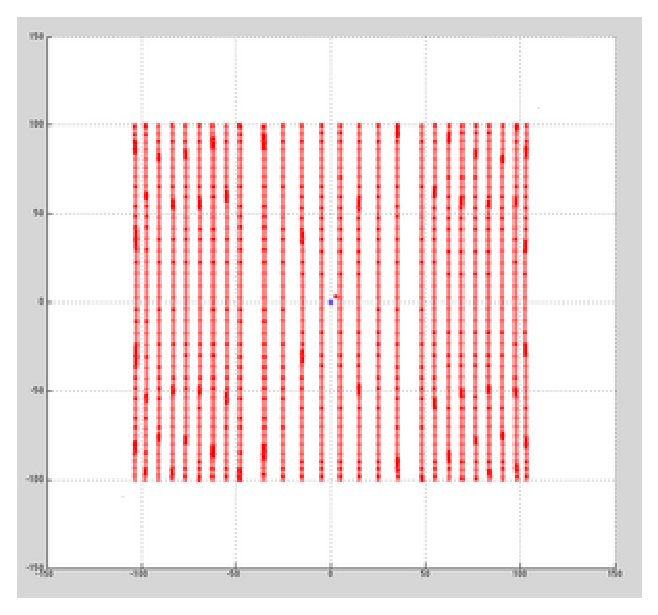
\includegraphics[width=1.65in]{isocenter/images/simulation/coronal_distortion_1.eps}}}
    \centerline{\emph{(c) Coronal view.}}\medskip
  \end{minipage}
%\hfill
%
\caption{\emph{Phantom modeling with small distortions}} \label{fig:3}
%
\end{figure}



Distortion in the sum of spherical harmonics is coupled in the x and y directions (orthogonal to axis), making the z axis independent.  Noise and distortion are thus very different in the z direction as opposed to the x-y plane.  We break down the gradient isocenter coordinate estimation into two big steps: estimation of z coordinate and estimation of x,y coordinate.

\subsubsection{Z-Coordinate Estimation}

Since the distortion model is based on sum of spherical harmonics, the shape of the distorted data for each tube is an even polynomial function. Figure~\ref{fig:3} shows that the realistic distortion is quite small, being about a maximum of 2 pixels, and the smaller the distortion the more sensitive the problem becomes.  With the first four terms of sum of spherical harmonics, the shape of the each tube can be seen as part of a polynomial function of 4th degree. Since the data points of tubes only represent the middle section of the 4th degree polynomial function, it is also very similar to a shape of quadratic function.  The offset between the largest distortion and the smallest distortion can be as small as 1mm.  With such a small margin, it is more practical to fit the data points to simpler model than a 4th degree polynomial.  Only the first spherical harmonic is needed in order to estimate the point where gradient is zero to measure the isocenter.  Furthermore, the first term of the sum of spherical harmonics has the largest signal to noise ratio, so we use a quadratic model to fit the data points.

We can see the distorted tube models' middle part is bending toward the center with both end bending outward.
If we were to fit each tubes to a parabola and locate the point where its gradient is zero, that point's
z-coordinate should be the same as the z-coordinate of the gradient isocenter of the magnetic field.  The z-coordinate is measured for all 64 tubes and the result averaged.  The resulting estimation is within $0.1$ mm of the actual z-coordinate.

\subsubsection{X,Y Coordinate Estimation}

The estimation of the x and y coordinates of the isocenter is the more difficult problem.
We are assuming that the difference between the distortion on x and y direction are so small that we can
treat them as if they are the same.  When this is not true, the errors on the isocenter location will be asymmetric, and it will be even more important to maintain a good numerical method to estimate the isocenter.  With that in mind, the distorted data of a tube should all stay on a plane which isocenter is also in. The intersection of such planes from each tube should be a line that
goes through isocenter. Using the isocenter estimated from previous step we should obtain an estimation
of x and y coordinate.

Since the tubes were aligned to the z-axis to reduce magnetic field distortion by the tubes, the range of data in the z-direction is of necessity larger.  In the x-y plane the range of points is controlled by the distortion, and is thus only a few pixels.  The resulting equations are highly sensitive, requiring careful handling in our numerical algorithm.

The equation of a plane in three dimensions is as follows.
\begin{eqnarray}
ax + by + cz + d & = & 0 \label{eq:plane}
\end{eqnarray}

Rewriting eq~\ref{eq:plane} with the measured data, we can solve for the plane each tube lies in.  This in turn can be used to find the intersection of the planes, which is the isocenter.
\begin{eqnarray}
-\frac{b}{a}y - \frac{c}{a}z - \frac{d}{a} & = & x \label{eq:x_orient}\\
\begin{bmatrix}
  y_0  & z_0 & 1 \\
  \vdots & \vdots & \vdots \\
  y_n & z_n & 1 \\
\end{bmatrix}
\begin{bmatrix}
-b/a\\
-c/a\\
-d/a
\end{bmatrix}
& = &
\begin{bmatrix}
x_0 \\
\vdots\\
x_n
\end{bmatrix} \nonumber\\
-m_x & = & \frac{b}{a} \nonumber\\
 k_x & = & - \frac{c}{a}z_{iso} - \frac{d}{a} \nonumber\\
  x  & = & -m_x y + k_x \nonumber\\
\begin{bmatrix}
1 \; m_x
\end{bmatrix}
\begin{bmatrix}
x \\
y
\end{bmatrix}
& = &
k_x \label{eq:x_est}
\end{eqnarray}

Note that eq~\ref{eq:plane} can be rewritten so either x or y is independent, which affects the error in standard least squares.  This becomes particularly important when the non-linearity is not the same in the x and y directions, as scaling is also well known to cause problems for least squares.
\begin{eqnarray}
-\frac{a}{b}y - \frac{c}{b}z - \frac{d}{b} & = & y \label{eq:y_orient}\\
\begin{bmatrix}
  x_0  & z_0 & 1 \\
  \vdots & \vdots & \vdots \\
  x_n & z_n & 1 \\
\end{bmatrix}
\begin{bmatrix}
-a/b\\
-c/b\\
-d/b
\end{bmatrix}
& = &
\begin{bmatrix}
y_0 \\
\vdots\\
y_n
\end{bmatrix} \nonumber\\
-m_y & = & \frac{a}{b} \nonumber\\
 k_y & = & - \frac{c}{b}z_{iso} - \frac{d}{b} \nonumber\\
  y  & = & -m_y x + k_y \\
\begin{bmatrix}
1 \; m_y
\end{bmatrix}
\begin{bmatrix}
y \\
x
\end{bmatrix}
& = &
k_y \label{eq:y_est}
\end{eqnarray}


% \begin{eqnarray}
% -\frac{a}{b}y - \frac{c}{b}z - \frac{d}{b} & = & y
% \end{eqnarray}

As we can see from figure~\ref{fig:4}, by using equation~\ref{eq:x_orient} and equation~\ref{eq:y_orient} to estimate
planes in figure~\ref{fig:4}(b) and \ref{fig:4}(d) respectively we get and quite accurate x and y coordinate
estimate. However, when you swap the choice of equations, even though they are mathematically identical,
they make a huge numeric difference as shown in \ref{fig:4}(a) and \ref{fig:4}(b).

\begin{figure}[htb]

  \begin{minipage}[b]{0.48\linewidth}
    \centering
    \centerline{\mbox{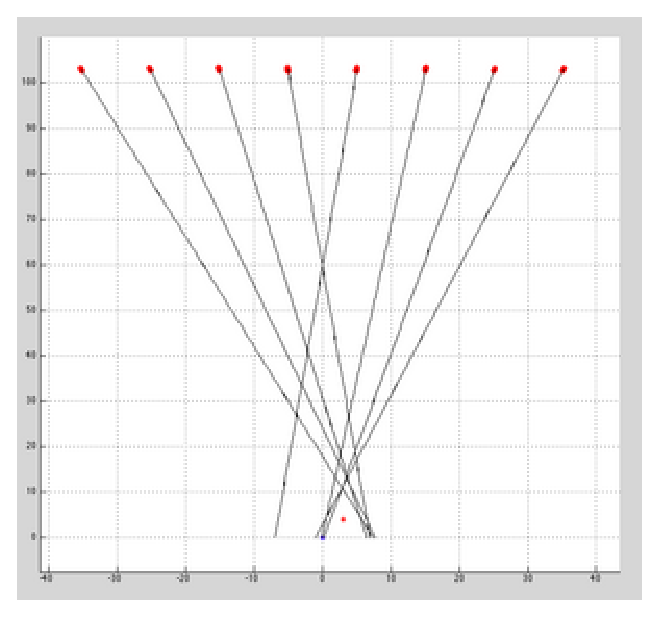
\includegraphics[width=1.65in]{isocenter/images/simulation/tube_plane_large_error_y.eps}}}
    \centerline{\emph{(a) LS fit with y orientation.}}\medskip
  \end{minipage}
  \hfill
  \begin{minipage}[b]{0.48\linewidth}
    \centering
    \centerline{\mbox{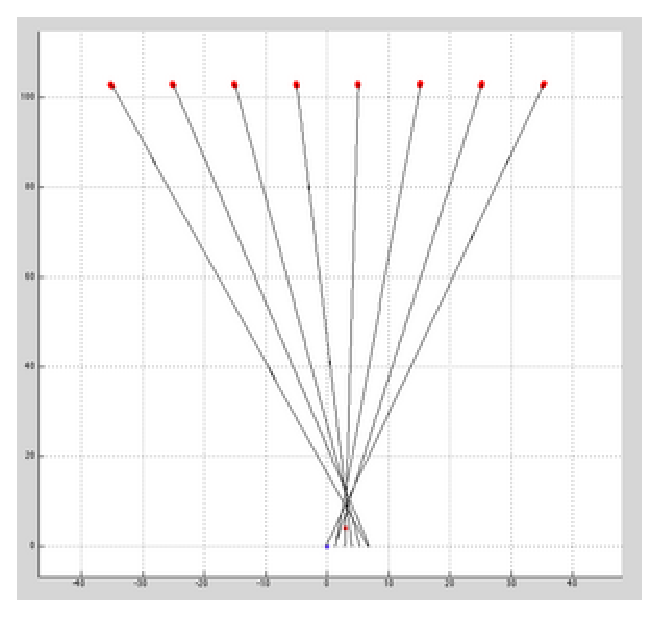
\includegraphics[width=1.65in]{isocenter/images/simulation/tube_plane_small_error_x.eps}}}
    \centerline{\emph{(b) LS fit with x orientation.}}\medskip
  \end{minipage}
  \begin{minipage}[b]{0.48\linewidth}
    \centering
    \centerline{\mbox{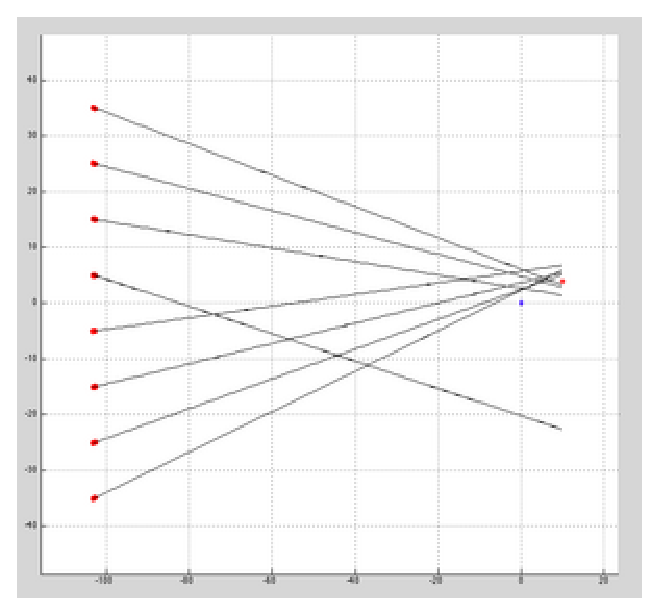
\includegraphics[width=1.65in]{isocenter/images/simulation/tube_plane_large_error_x.eps}}}
    \centerline{\emph{(c) LS fit with x orientation.}}\medskip
  \end{minipage}
  \hfill
  \begin{minipage}[b]{0.48\linewidth}
    \centering
    \centerline{\mbox{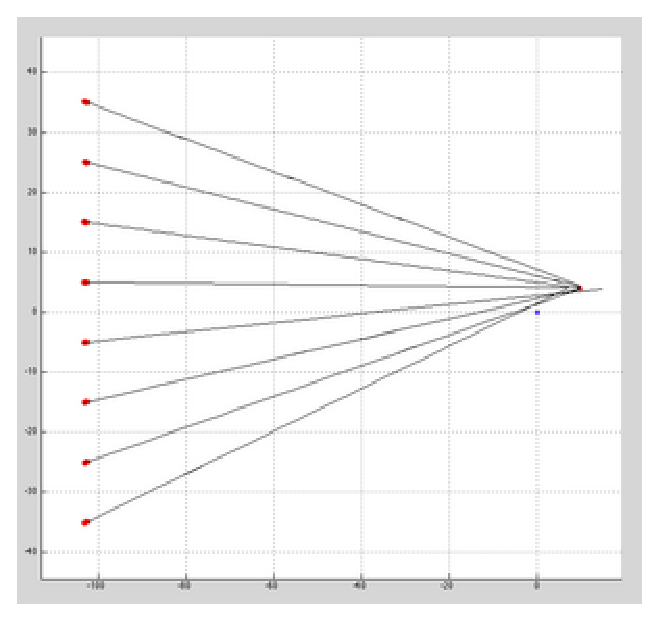
\includegraphics[width=1.65in]{isocenter/images/simulation/tube_plane_small_error_y.eps}}}
    \centerline{\emph{(d) LS fit with y orientation.}}\medskip
  \end{minipage}
\caption{\emph{Phantom modeling with distortion, showing differences in isocenter estimates due to how the LS equation is oriented.}} \label{fig:4}
%
\end{figure}

When estimating the x-y coordinate using least square we should keep in mind that least square assumes
there is no observation error, it will only try to correct one side of the equation depending on how it
is setup. With this in mind, we uses equation \ref{eq:x_est} for x coordinate estimation and \ref{eq:y_est}
for y estimation. For the tubes on the diagonal planes, as we can see in fig\ref{fig:diagonal},
they offers neither a good data for x nor y coordinate estimation as compared to fig~\ref{fig:4} (b) and (d). So in order to utilize the diagonal
tubes we have to rotate these tubes to either x or y plane, and get an estimation of a rotated x-y
coordinate, then rotate the rotated x-y coordinate back and average it with original x-y coordinate
estimation.

\begin{figure}[htb]

  \begin{minipage}[b]{0.48\linewidth}
    \centering
    \centerline{\mbox{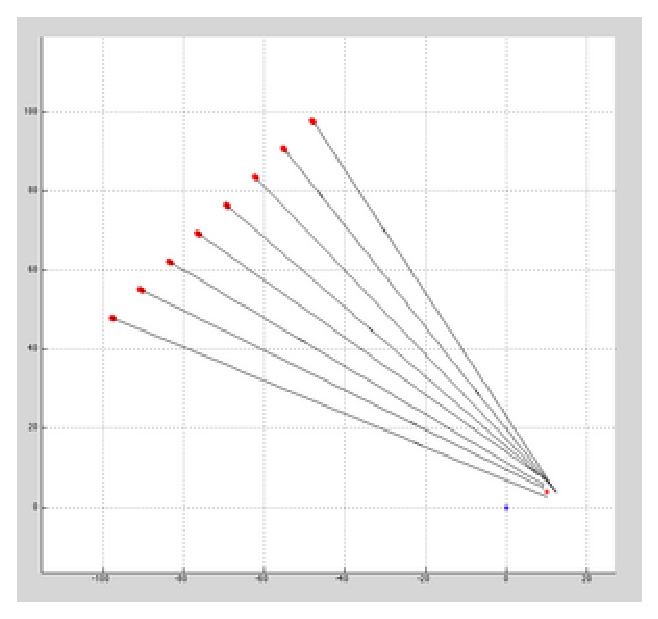
\includegraphics[width=1.65in]{isocenter/images/simulation/tube_plane_diagonal_using_x.eps}}}
    \centerline{\emph{(a) LS using x orientation.}}\medskip
  \end{minipage}
  \hfill
  \begin{minipage}[b]{0.48\linewidth}
    \centering
    \centerline{\mbox{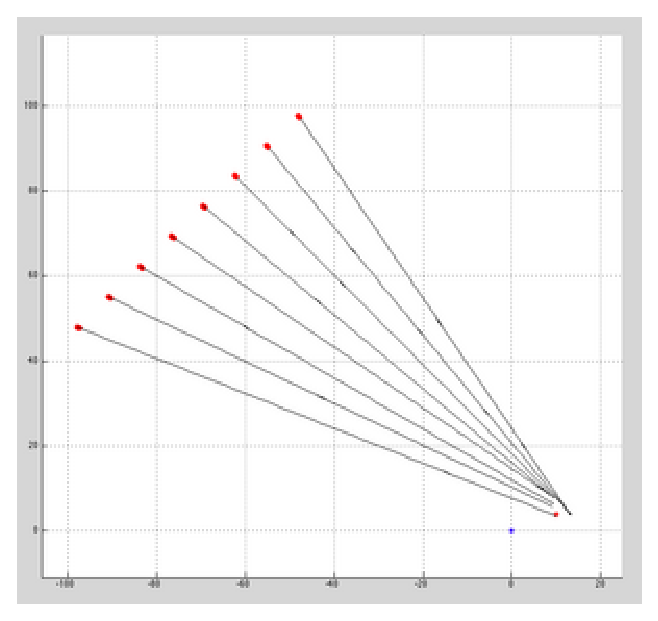
\includegraphics[width=1.65in]{isocenter/images/simulation/tube_plane_diagonal_using_y.eps}}}
    \centerline{\emph{(b) LS using y orientation.}}\medskip
  \end{minipage}
\caption{\emph{Phantom modeling with distortion, showing how diagonal tube planes without rotation do not improve the estimates produced.}} \label{fig:diagonal}
%
\end{figure}

In order to obtain a good estimate, we thus must separate the estimation of x and y, as well as rotate the diagonal oriented tube planes and then separate the estimation of x and y and rotate back.  We refer to this algorithm as Rotated
Separable Least Squares (RSLS). We now present the RSLS algorithm to estimate x-y coordinate of gradient isocenter as follows:

\begin{enumerate}
\item Use equation~\ref{eq:x_orient} to estimate tube planes for tubes at upper and lower surfaces.
\item Solve equation~\ref{eq:x_est} for x and y, but only use x for x coordinate.
\item Use equation~\ref{eq:y_orient} to estimate tube planes for tubes at left and right surfaces.
\item Solve equation~\ref{eq:y_est} for y and x, but only use y for y coordinate.
\item Rotate diagonal tubes $\pi/4$, and repeat steps 1-4.
\item Rotate x-y coordinate obtained from previous step by $-\pi/4$.
\item Average the x-y coordinate from previous step with x-y coordinate calculated from step 2 and step 4 for final x-y estimation.
\end{enumerate}

Alternatively, after obtaining the plane equation parameters we can put everything into one matrix and do
a one time estimation using either least square or total least square. In table~\ref{table:symmetric}, we
can see the comparison of accuracy of estimating an isocenter at $[4 \; 4\; 3]$ using different methods.
Least square tends to lean toward one coordinate
more depends on setup, while total least square has an accurate and very balanced result due to the property
that it will try to correct errors on both side of the equation. In the contrast, our method has best
properties of both methods:

\begin{itemize}
  \item It is accurate. For both x and y coordinate it does a better job than total least square, much better than least square's worst case and very close to least square's best case.
  \item It has very balanced result. Both x and y coordinates are very close the correct result equally just like total least square.
  \item It has very tight error boundaries. After 200 runs, it's error is tighter than standard least square.
\end{itemize}

Therefore, our estimation method is a good alternative to traditional least square or total least square methods. Although it might require more computation, it could be easily dealt by modern GPU computing. And due to the fact that each least square estimation has relative small matrix, and each estimation is independent of each other, it is very close to ``embarrassingly parallel'' type of problems and makes it easy to solve.


%KES the other is too nice for all examples so we need to show the ugliness.  I don't have the data, so I am setting what
%    I recall from our talk last night.  It will need your data.

In table~\ref{table:symmetric}, the test is run using a symmetric x-y axis distortion. We can see that all three methods performed very well. RSLS method's result is slightly better than Total Least Squares (TLS), and one on y axis it is better than standard Least Squares method.

%KES - what is two LS method and what is one LS method?  must explain in text?
%      is one traditional and the other our new method?
\begin{table}
  \begin{tabular} {| l | r | r | r | r | r | r |}
    \hline
    & $\bar{x}$ & $\sigma_x$ & err & $\bar{y}$ & $\sigma_y$ & err  \\
    \hline
    RSLS  & 3.9709 & 0.1068  & 0.0291 & 3.9677 & 0.1008 & 0.0323\\
    \hline
    LS & 3.9950 & 0.1118 & 0.0050   & 3.9414 & 0.1011 & 0.0586 \\
    \hline
    TLS  & 4.0800 & 0.1035  & 0.0800   & 4.0800 & 0.0964 & 0.0800 \\
    \hline
  \end{tabular}
  \caption{\emph{Average of 200 runs using different methods for estimating the isocenter at $[4 \; 4 \; 3]$ in the presence of symmetrical distortion}} \label{table:symmetric}
\end{table}


When the distortion is not symmetrical the issue of proper estimation becomes crucial. In table~\ref{table:nonsymmetric}, we show the result of using non-symmetrical distortion in which the y direction was set to be twice the distortion in the x. In this test, TLS method's result is the worst, off by a few millimeters.  Both LS and RSLS show comparable degradation of performance in x.  LS shows degradation in the estimation of y as well, but RSLS, since it is separable, does not experience any degradation of it. Only the RSLS's result remains quite accurate. This shows the advantage of RSLS over the other two traditional methods.


\begin{table}
  \begin{tabular} {| l | r | r | r | r | r | r |}
    \hline
    & $\bar{x}$ & $\sigma_x$ & err & $\bar{y}$ & $\sigma_y$ & err \\
    \hline
    RSLS & 3.8073 & 0.1117 & 0.1927   & 3.9838 & 0.1059 & 0.0162 \\
    \hline
    LS  & 4.2191 & 0.1117    & 0.2191 & 3.8765 & 0.1003 & 0.1235 \\
    \hline
    TLS  & 9.5744 & 0.2616 & 5.5744   & 8.6905 & 0.2393 & 4.6905 \\
    \hline
  \end{tabular}
  \caption{\emph{Average of 200 runs using different methods for estimating the isocenter at $[4 \; 4 \; 3]$ in the presence of non-symmetrical distortion }} \label{table:nonsymmetric}
\end{table}


\subsection{Conclusion}
In this work, we developed a new numerical algorithm to accurately determine the gradient isocenter
of MRI scanners based on a new distortion correction phantom. Knowledge of the gradient isocenter is an essential part of gradient-nonlinearity correction methods.  We have shown that the method used in this work to estimate the gradient isocenter is a good alternative to more traditional estimation methods such as least squares and total least squares. The new algorithm is particularly suited when the image data are extremely sensitive to the presence of noise and asymmetric distortion. Using simulated (but realistic) distortion data, it was shown, that the resulting estimated isocenter was within $0.2$ mm of the actual gradient isocenter, leading to a better estimate than the currently used DICOM coordinate center.


\Chapter{Data Extraction}
\label{data_extraction}


\section{Water Tank Distance Measurement Extraction}
\label{ct_tank}

\subsection{CT Scan overview, target surfaces}
Due to the limitation of manufacture equipments, water tank at each end can only be guaranteed that their
surfaces are parallel \footnote{what's the error?} to each other, their accurate distances betweeen each other
are unknown. We decided to perform a CT scan\footnote{what's the CT's error} on the phantom, then collect each
surfaces' data points through coronal view CT images. With enough data points on each surface, we should be
able to have a good estimation of the distances with between each pair of surfaces. \footnote{brief outline of full algorithm}

\begin{figure}[htb]
  \begin{minipage}[t]{2.75in}
    \centering
    \centerline{\mbox{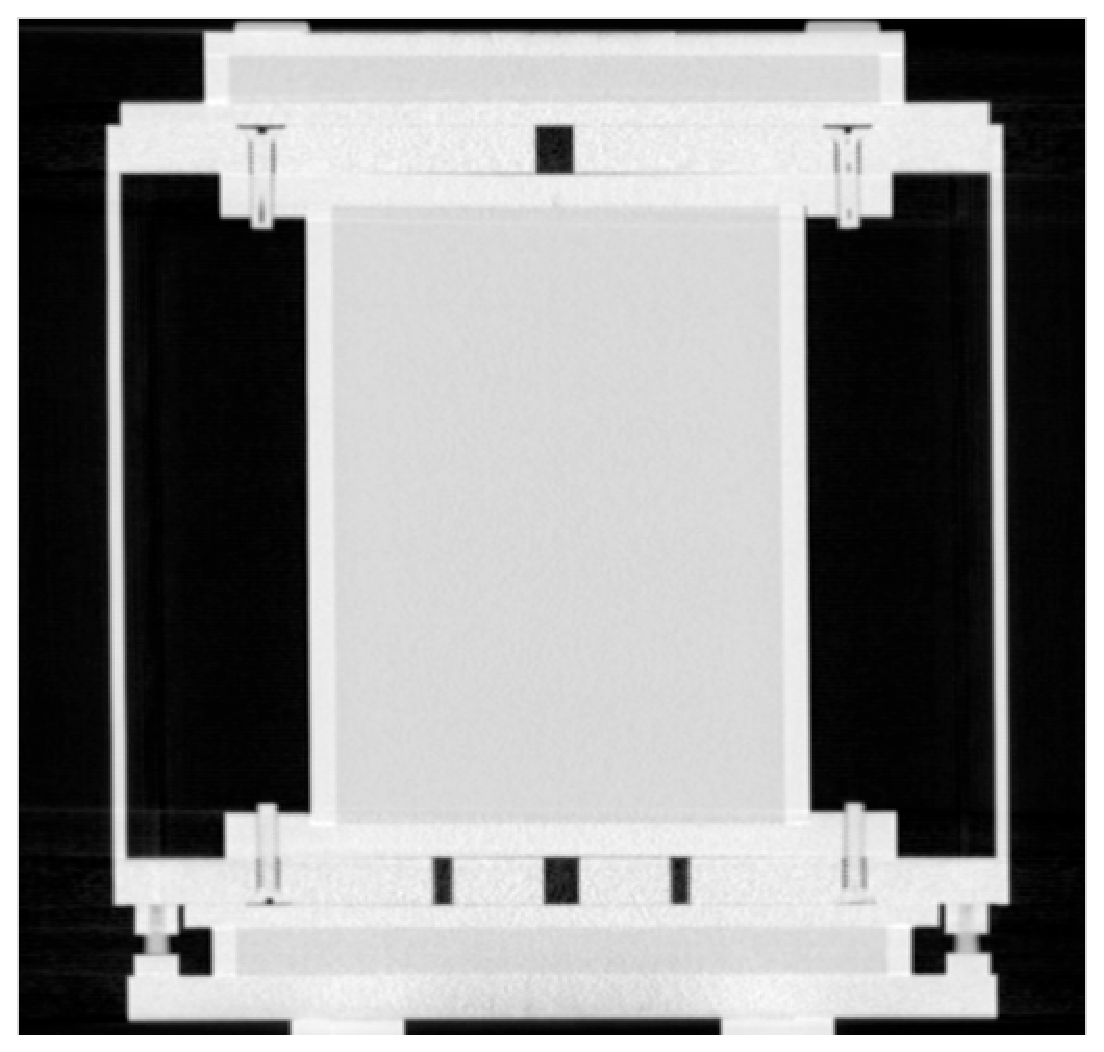
\includegraphics[width=2.75in]{data_extraction/images/targets/ct_coronal_mid_slice.eps}}}
    \centerline{\emph{(a) Coronal view, center slice}}
  \end{minipage}\medskip
  \begin{minipage}[t]{2.75in}
    \centering
    \centerline{\mbox{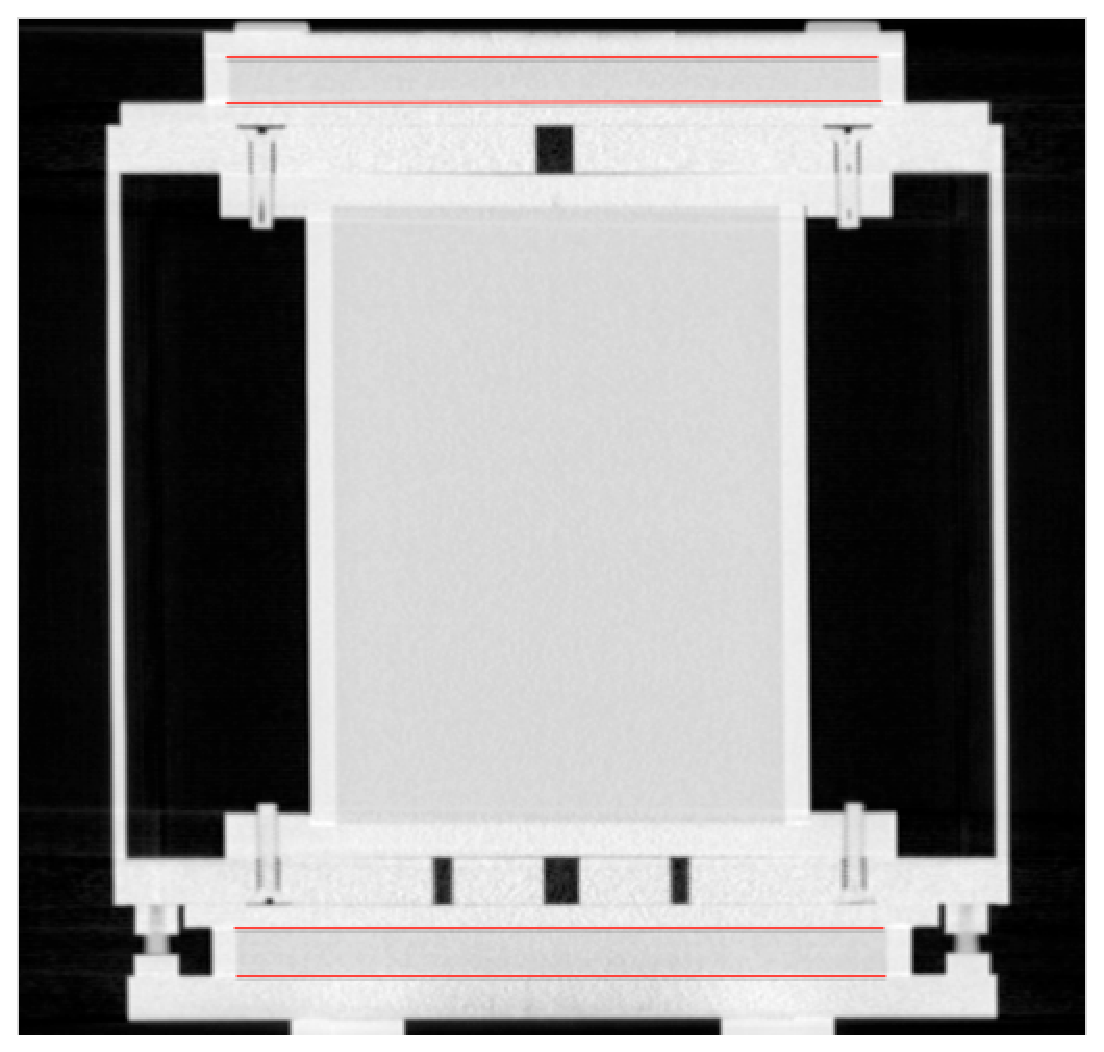
\includegraphics[width=2.75in]{data_extraction/images/targets/ct_coronal_mid_slice_marked_surface.eps}}}
    \centerline{\emph{(b) Marked target surfaces}}
  \end{minipage}
\end{figure}

Above images indicates the target feature we are looking for inside a typical coronal view of CT image.

\subsection{Canny Edges}

The obvious method is to extract the data points is to apply an edge detection algorithm on the image, then
iterate through the resulting edge image to collection the desired lines. However, the resulting edge image from
this approach often contain fair amount of noise edges some of which overlap with the desired edges we are looking
for. This problem is illustrated in figure \ref{fig:canny_ct_141}, \ref{fig:canny_ct_270} and \ref{fig:canny_ct_276}.
 
\begin{figure}[htb]
  \begin{minipage}[t]{2.75in}
    \centering
    \centerline{\mbox{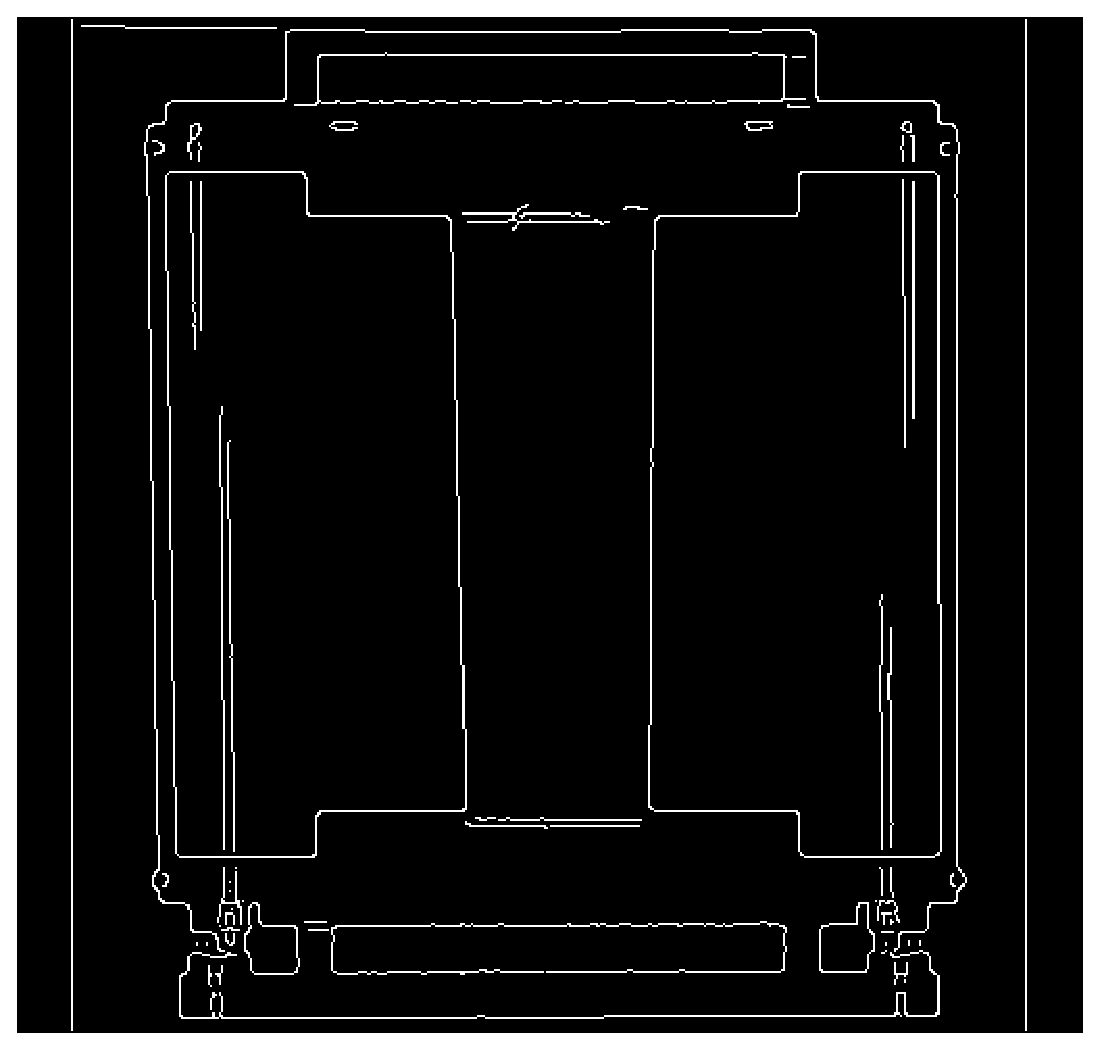
\includegraphics[width=2.75in]{data_extraction/images/canny/default/20121017_141.eps}}}
    \centerline{\emph{(a) Default parameters}}
  \end{minipage}\medskip
  \begin{minipage}[t]{2.75in}
    \centering
    \centerline{\mbox{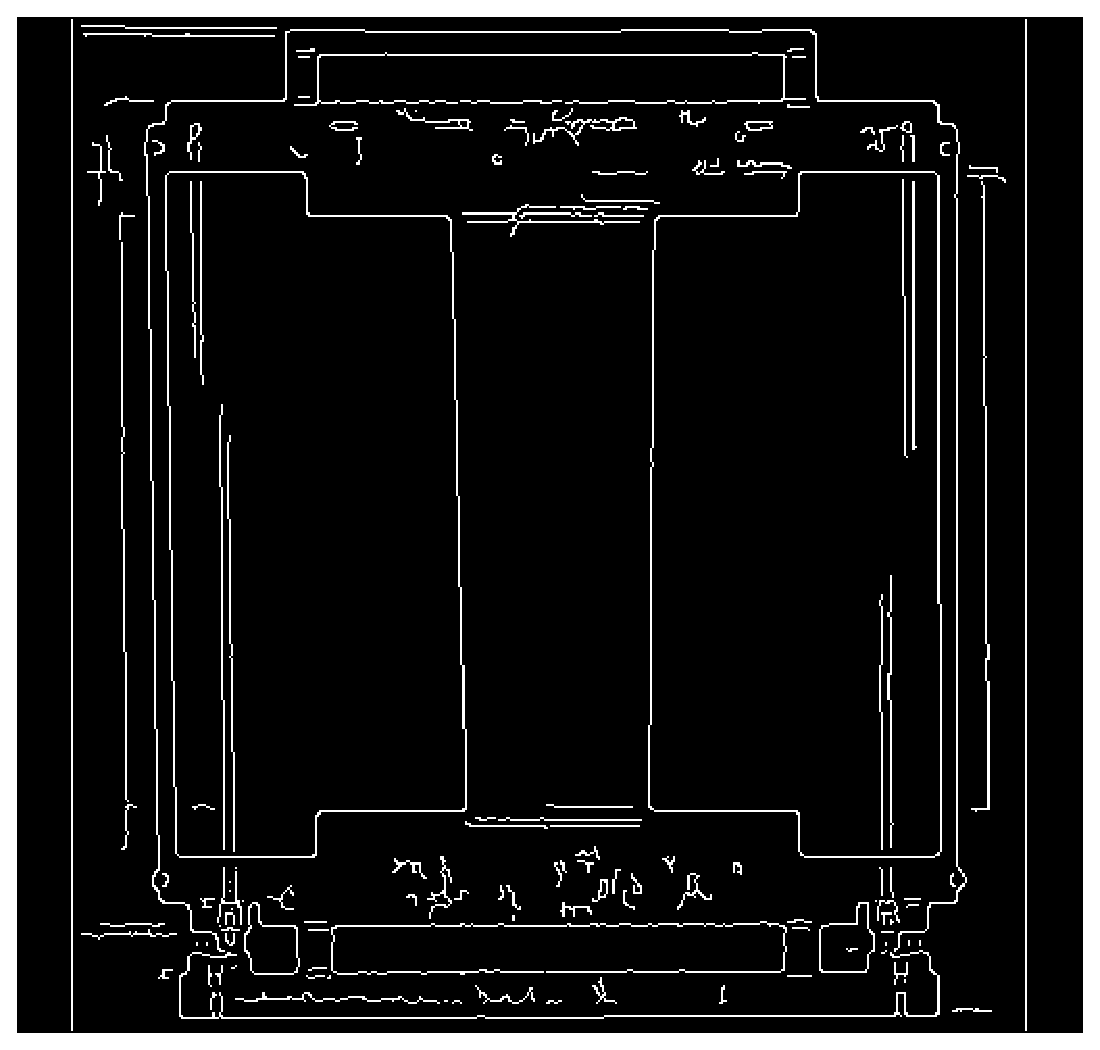
\includegraphics[width=2.75in]{data_extraction/images/canny/0.01_0.02/20121017_141.eps}}}
    \centerline{\emph{(b) Low threshold 0.01, high threshold  0.02}}
  \end{minipage}
  \begin{minipage}[t]{2.75in}
    \centering
    \centerline{\mbox{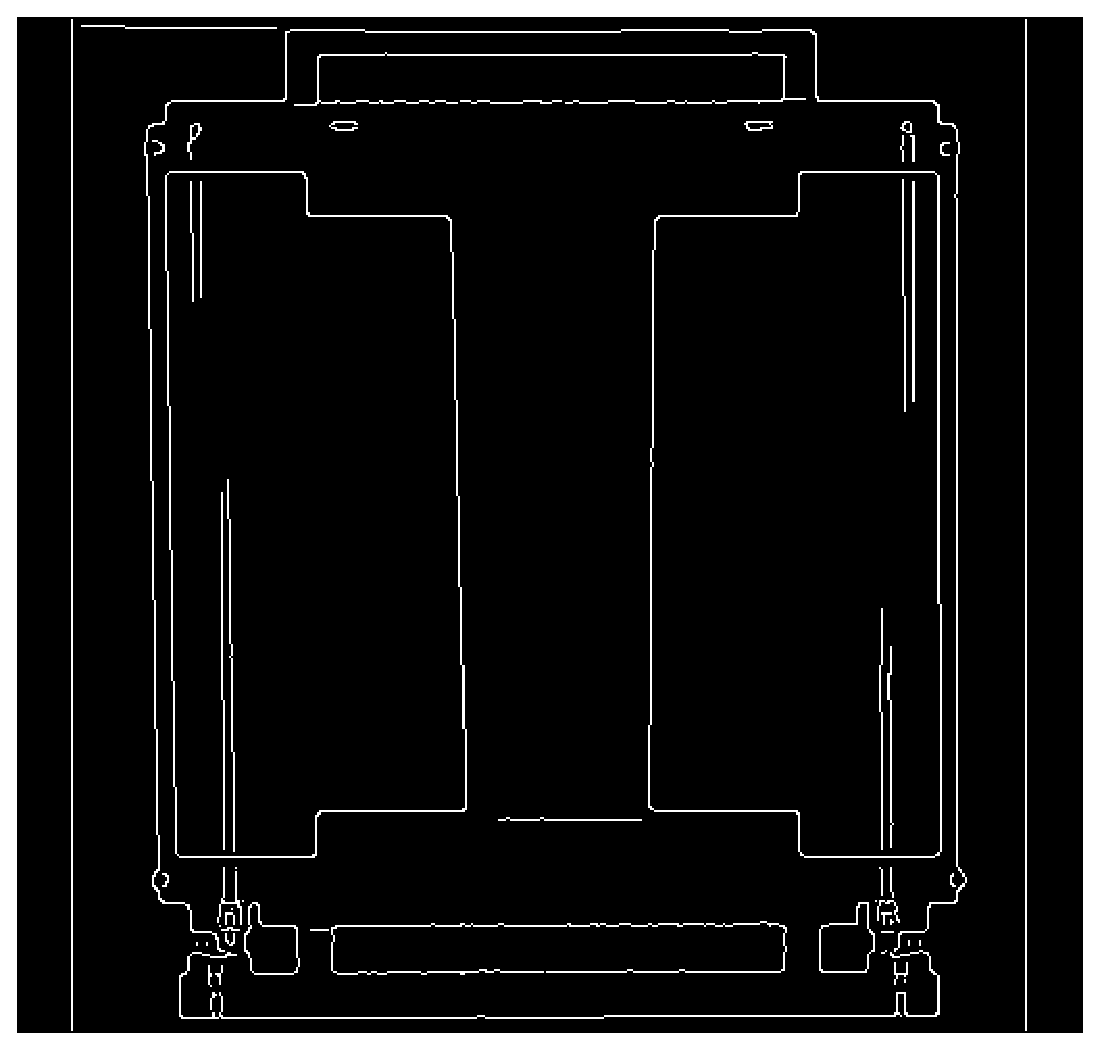
\includegraphics[width=2.75in]{data_extraction/images/canny/0.02_0.04/20121017_141.eps}}}
    \centerline{\emph{(c) Low threshold 0.02, high threshold  0.04}}
  \end{minipage}\medskip
  \begin{minipage}[t]{2.75in}
    \centering
    \centerline{\mbox{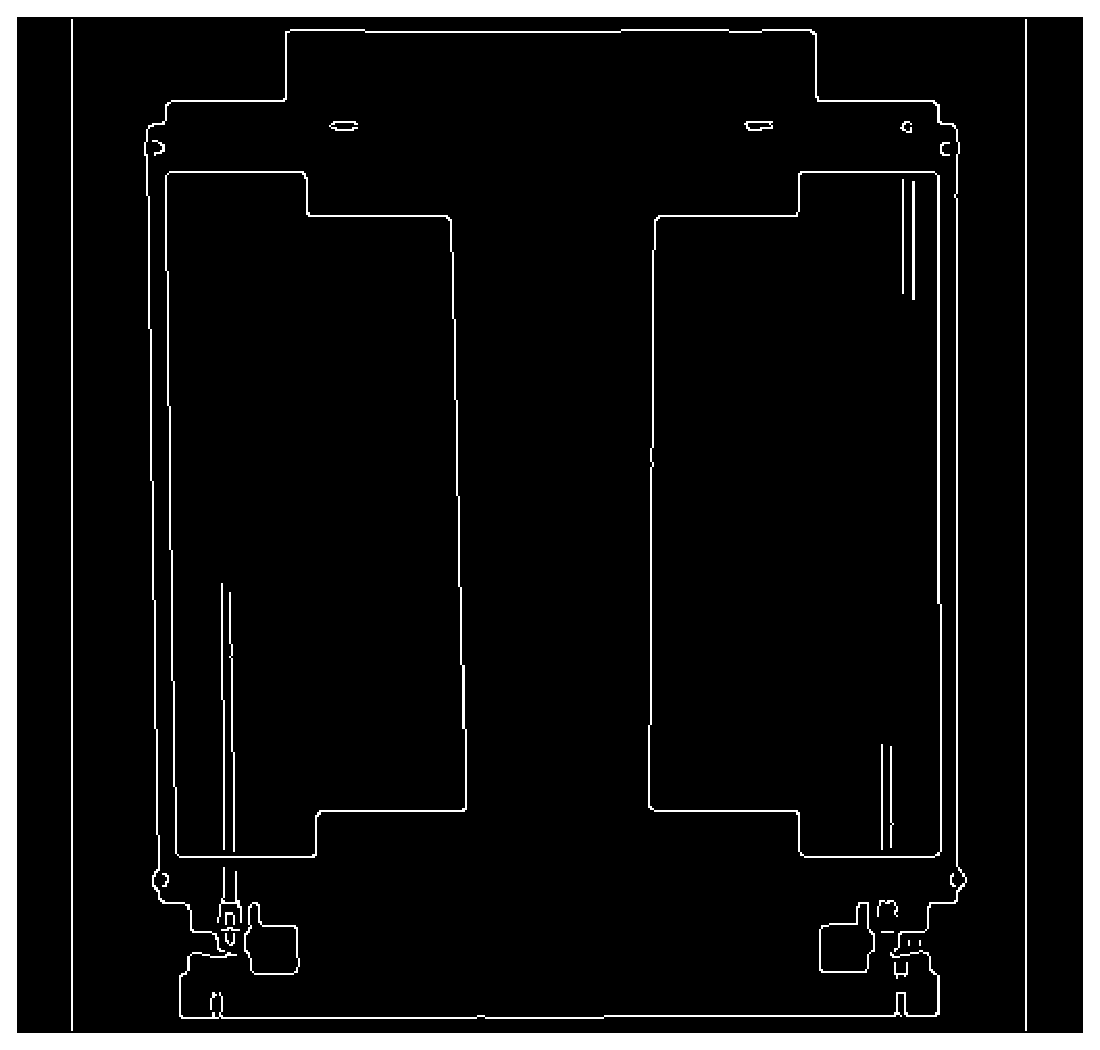
\includegraphics[width=2.75in]{data_extraction/images/canny/0.05_0.1/20121017_141.eps}}}
    \centerline{\emph{(d) Low threshold 0.05, high threshold  0.1}}
  \end{minipage}
  \caption{\emph{Canny algorithm applied to coronal sequence 141 with different parameters}} \label{fig:canny_ct_141}
\end{figure}


\begin{figure}[htb]
  \begin{minipage}[t]{2.75in}
    \centering
    \centerline{\mbox{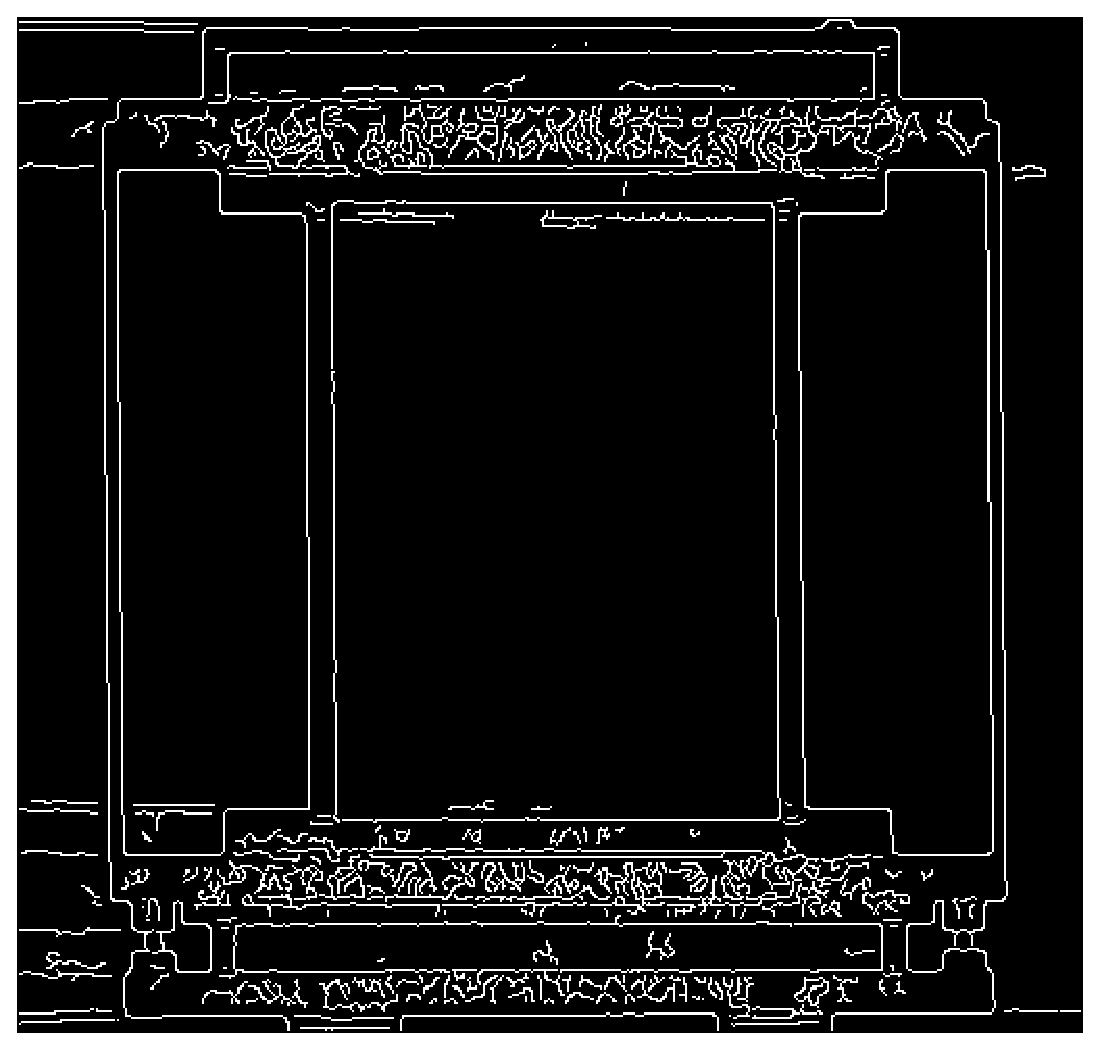
\includegraphics[width=2.75in]{data_extraction/images/canny/default/20121017_270.eps}}}
    \centerline{\emph{(a) Default parameter}}
  \end{minipage}\medskip
  \begin{minipage}[t]{2.75in}
    \centering
    \centerline{\mbox{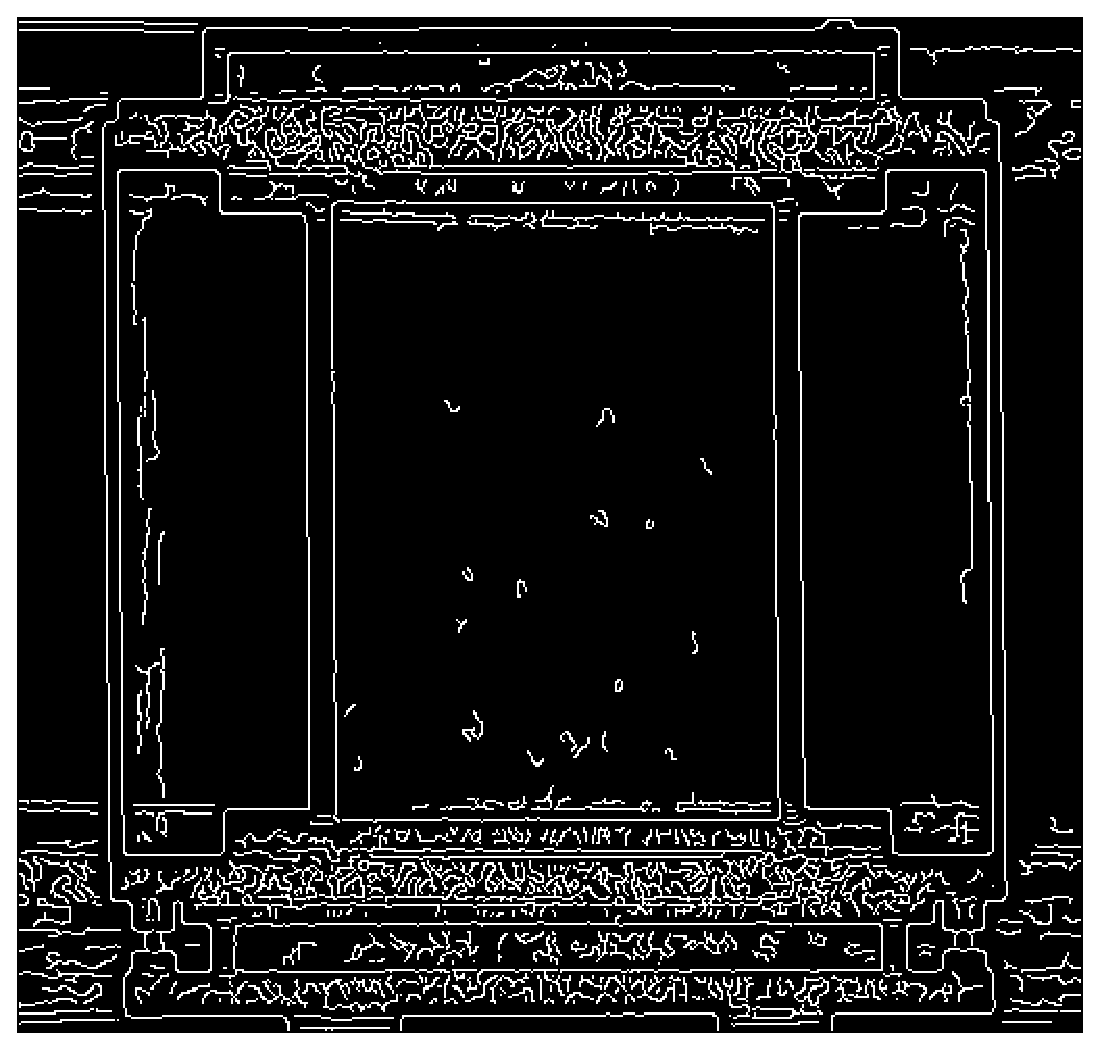
\includegraphics[width=2.75in]{data_extraction/images/canny/0.01_0.02/20121017_270.eps}}}
    \centerline{\emph{(b) Low threshold 0.01, high threshold  0.02}}
  \end{minipage}
  \begin{minipage}[t]{2.75in}
    \centering
    \centerline{\mbox{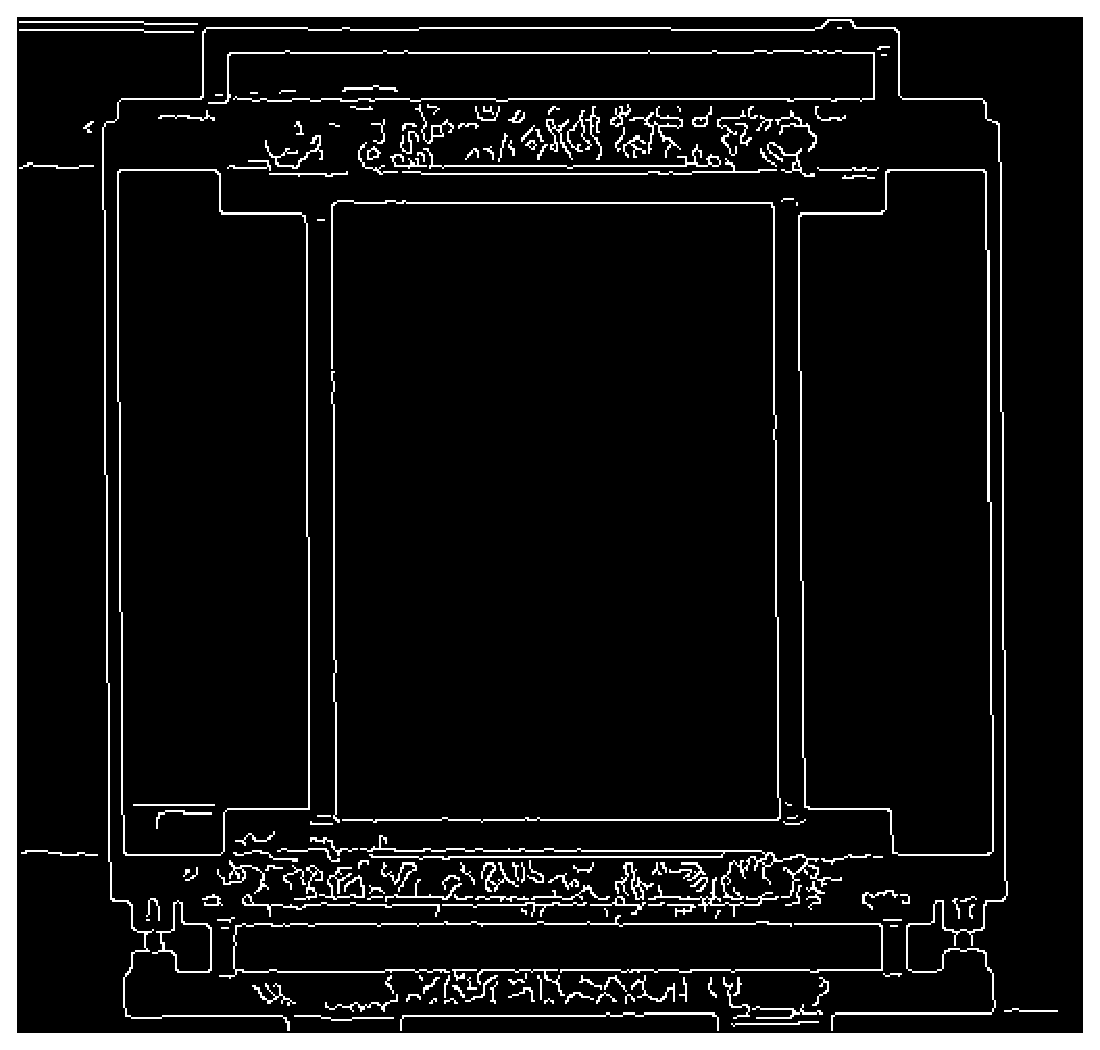
\includegraphics[width=2.75in]{data_extraction/images/canny/0.02_0.04/20121017_270.eps}}}
    \centerline{\emph{(c) Low threshold 0.02, high threshold  0.04}}
  \end{minipage}\medskip
  \begin{minipage}[t]{2.75in}
    \centering
    \centerline{\mbox{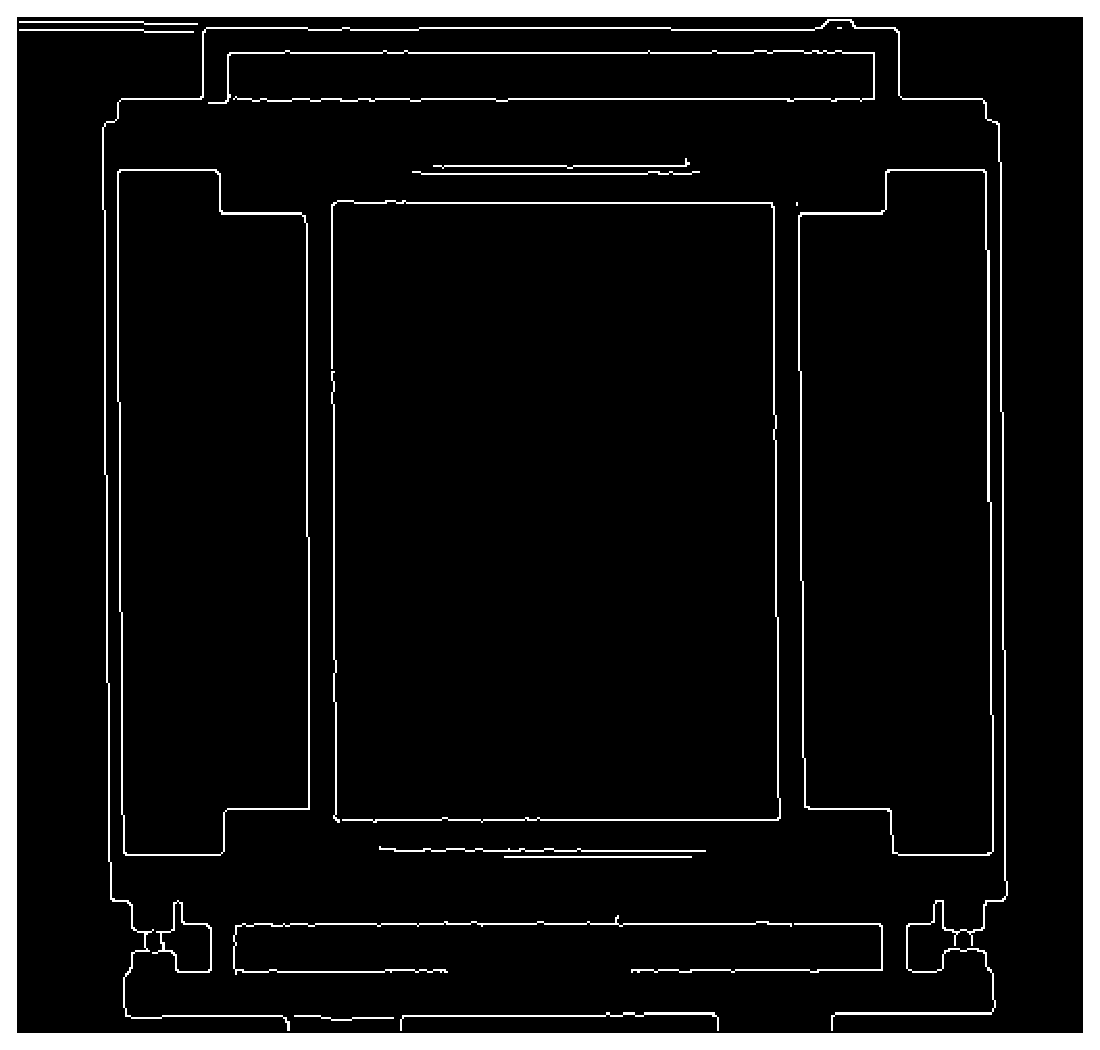
\includegraphics[width=2.75in]{data_extraction/images/canny/0.05_0.1/20121017_270.eps}}}
    \centerline{\emph{(d) Low threshold 0.05, high threshold  0.1}}
  \end{minipage}
  \caption{\emph{Canny algorithm applied to coronal sequence 270 with different parameters}} \label{fig:canny_ct_270}
\end{figure}

\begin{figure}[htb]
  \begin{minipage}[t]{2.75in}
    \centering
    \centerline{\mbox{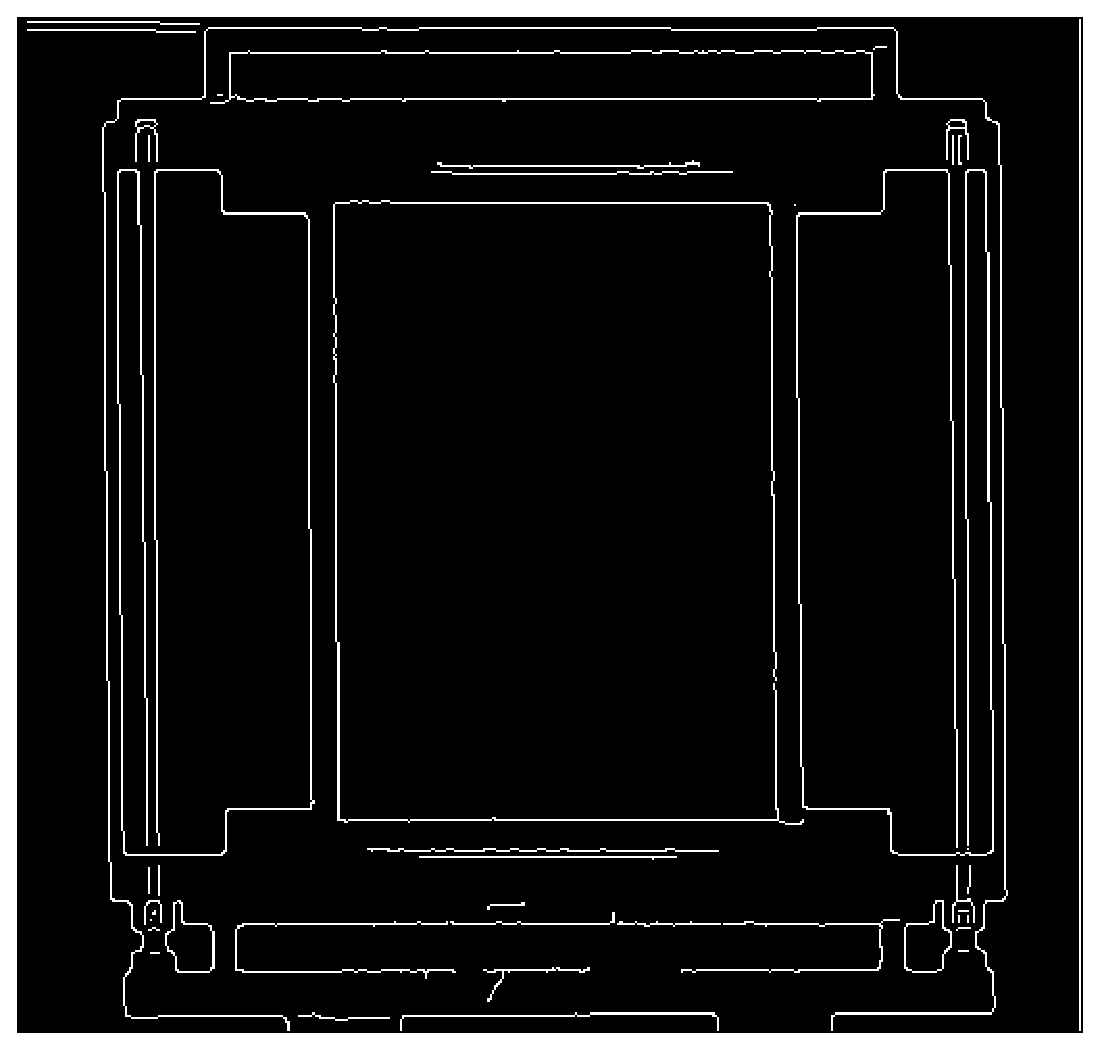
\includegraphics[width=2.75in]{data_extraction/images/canny/0.02_0.04/20121017_276.eps}}}
    \centerline{\emph{(f) Low threshold 0.02, high threshold  0.04}}
  \end{minipage}\medskip
  \begin{minipage}[t]{2.75in}
    \centering
    \centerline{\mbox{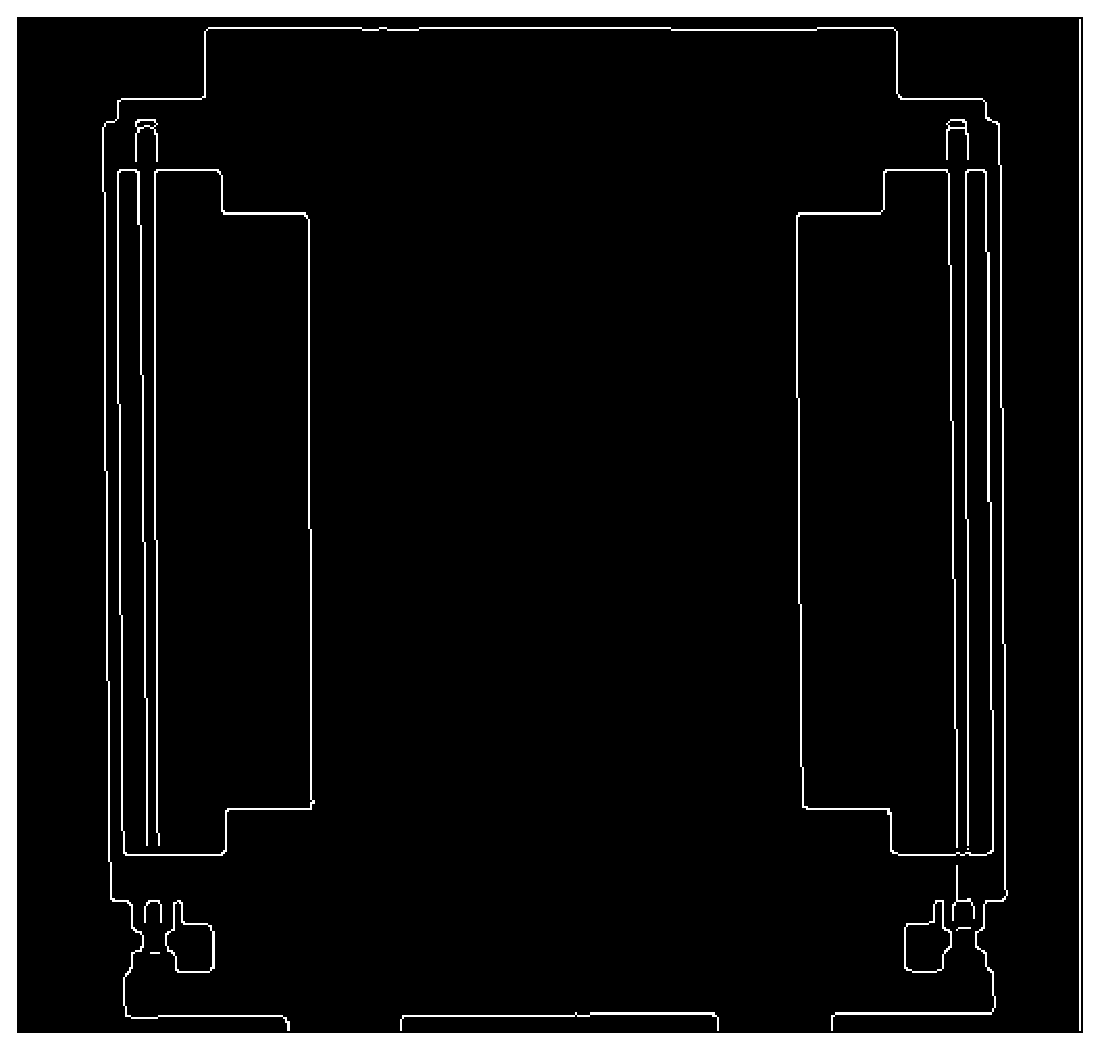
\includegraphics[width=2.75in]{data_extraction/images/canny/0.05_0.1/20121017_276.eps}}}
    \centerline{\emph{(h) Low threshold 0.05, high threshold  0.1}}
  \end{minipage}
  \caption{\emph{Canny algorithm applied to coronal sequence 276 with different parameters}} \label{fig:canny_ct_276}
\end{figure}

In figure \ref{fig:canny_ct_141}(a), we can see that Matlab's canny algorithm with default parameter gives 
descent edges when applied to image \#141. However, the same parameters will create many noisy edges in some other
images, e.g. \#270 in the same series in figure \ref{fig:canny_ct_270}(c). Setting higher threshold is able to
reduce those noisy edges as we can see in figure \ref{fig:canny_ct_270}(c), but that threshold will eliminate
some edges we are looking for as shown in \ref{fig:canny_ct_141}(c). 

To get rid of this noisy edges, different types algorithms might be involved, probably including validating
all the edges in an image,
which might involve multiple pass to the whole image, and in which case the process
could be slowed down by factor of several times. So if there is a simpler and faster way, it would be preferred
choice.

\subsection{Surface Location}

Since all objects we are looking for has a very uniform and distinct shape, we could start with finding a small 
regions each contains one object. In our case, the choice is very obvious. The objects we are looking for are
four straight lines at fixed location and parallel to each other. For images that contain those objects, they
should have them at almost exactly the same location with possibility of a few pixels offset due to potential
tiltness of the phantom during scan. If we choose a slice in the middle of the series, that should give us a
relatively smaller overall error margin both above and below the surface location on that particular slice
comparing to picking a slice at the beginning or at the end of the series which would give a relatively larger 
error on either above or below the surface location. Also the slice in the middle of series tends to have better 
quality. We would call this middle slice as surface location sample.

In the surface location sample, we would plot a histogram of gradient of the sum of middle 7 columns as shown
in figure \ref{fig:histograms_mid_coronal}(a) and a histogram of intensity distribution as shown in
figure \ref{fig:histograms_mid_coronal}(b). From figure \ref{fig:histograms_mid_coronal}(b), we can see that there
are three very obvious normal distribution in the graph. 
From left to right, they represent background noise signal, water signal and phantom tank signals respectively.
In figure \ref{fig:histograms_mid_coronal}(c), a zoomed in picture of the region between water signal distribution
and phantom tank distribution, we can see that two distributions' tails overlaps with each other. From the fact 
that the number of pixels in this overlap region is quite small and that this region is between two 
distributions, we can determine that most of them should be the pixels on the boundary between water and tank.
So, according to ranges of two distributinos as we can observer from the diagram, the range of difference
between tank signal and water signal should be somewhere between 40 to 300. However, since the difference we are
looking for is on the boundary of water and phantom tank, signals in those regions should tend to be close 
to each other. Therefore we should expect the to see spikes in gradient to be around $\pm40$. In figure
\ref{fig:histograms_mid_coronal}(a), we can clearly see six spikes that can be uniquely identified.
Their values are -41.8404, 44.2372, -36.2271, 50.4055, -40.9654 and 29.8124, and they are right around the 
predicted range. Thus, we can identify them with high confidence that they are on each of the boundary between
water and phantom tank.

With one pixel on each locations of the water and phantom tank boundaries are identified, 
we can also narrow down the 
location of each surface by specifying the surfaces are within the $\pm5$ rows of the row coordinate of each
identified pixels. The $\pm5$ rows should give enough room for any horizontal or vertical tiltness.

\begin{figure}[htb]
  \begin{minipage}[t]{2.75in}
    \centering
    \centerline{\mbox{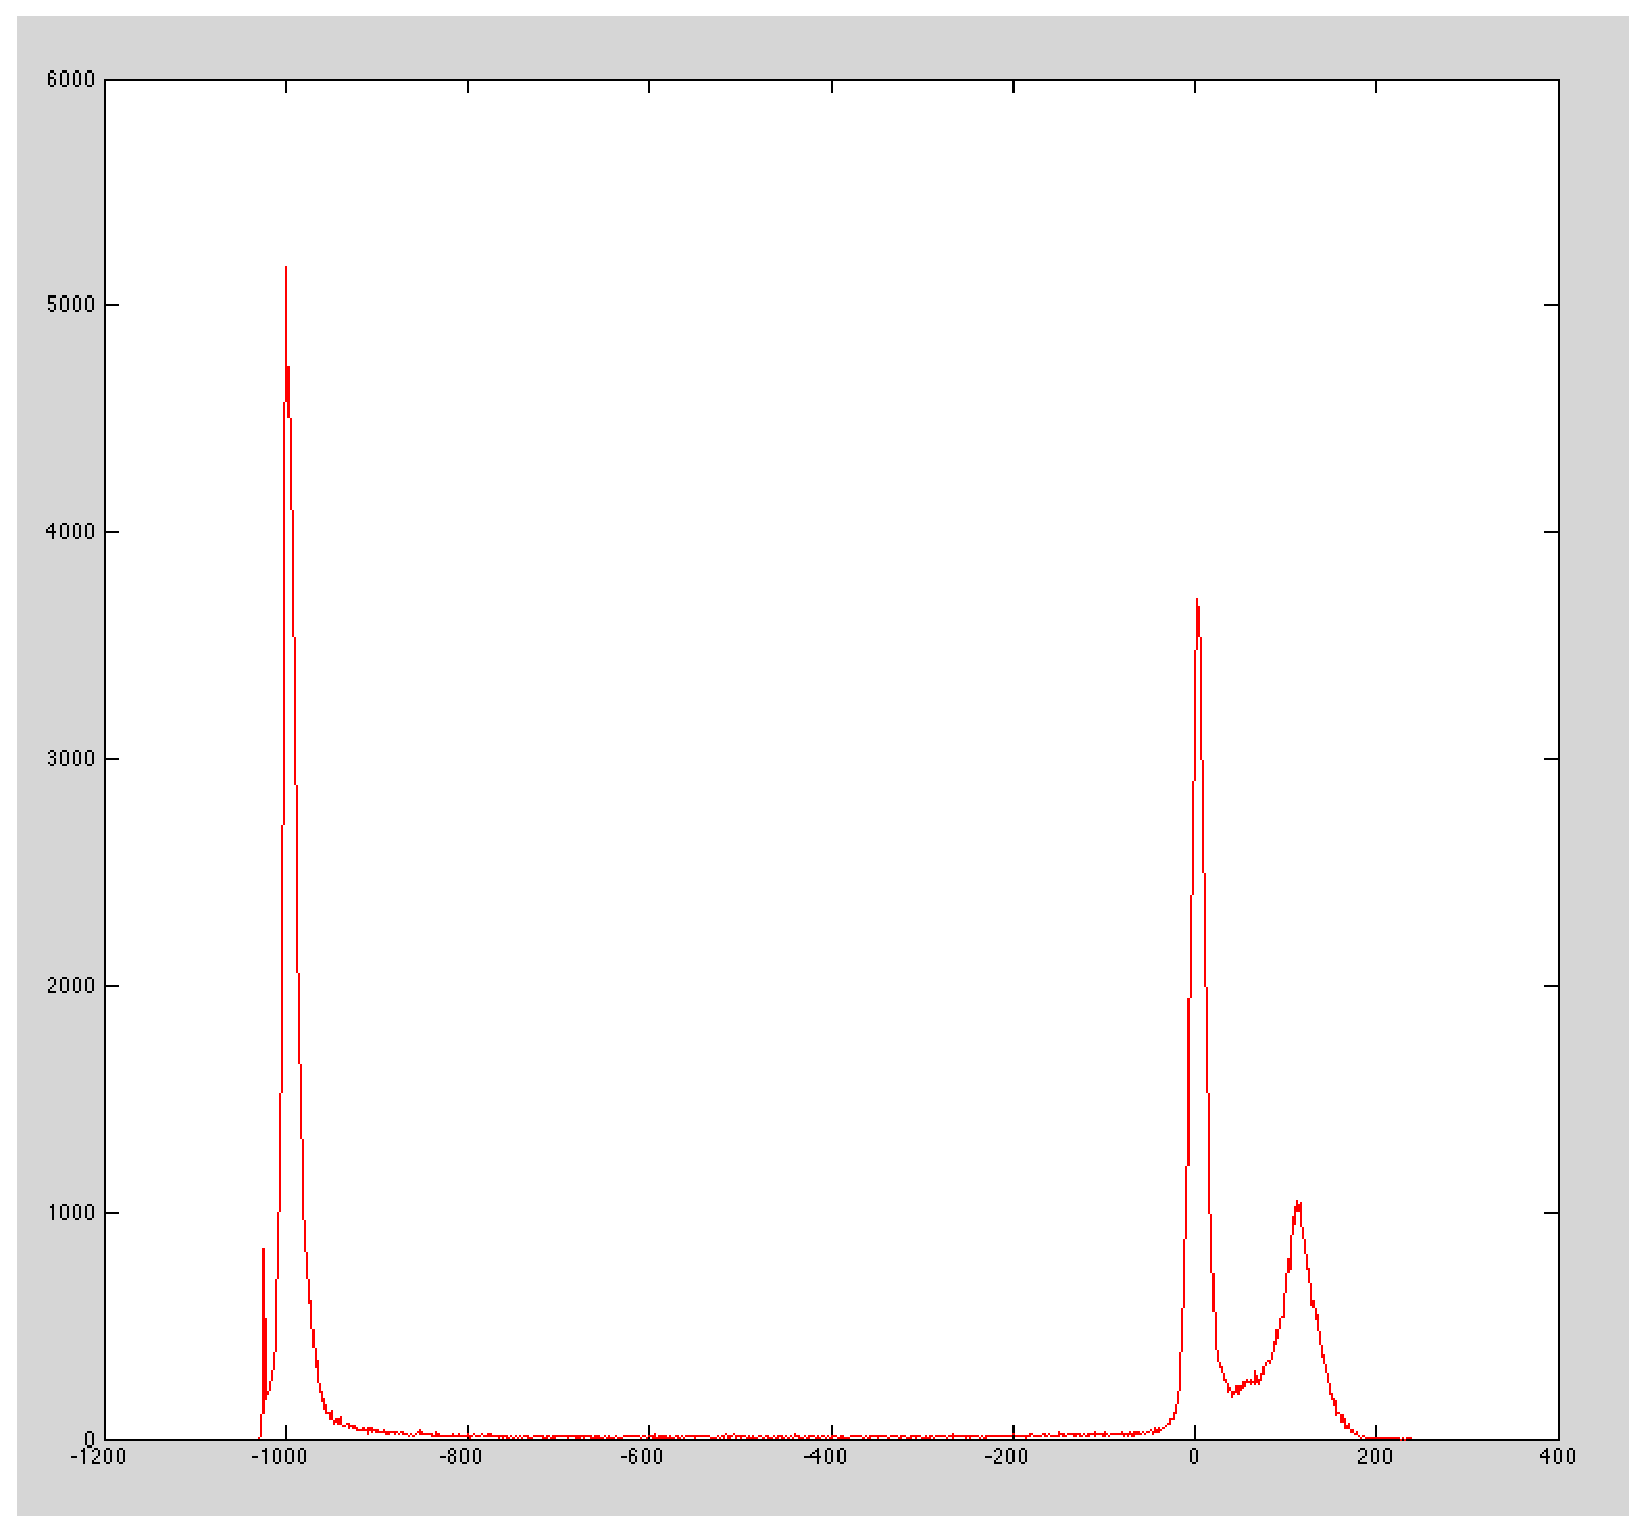
\includegraphics[width=2.75in]{data_extraction/images/mid_slice_histogram.eps}}}
    \centerline{\emph{(a) mid slice intensity histogram}}
  \end{minipage}\medskip
  \begin{minipage}[t]{2.75in}
    \centering
    \centerline{\mbox{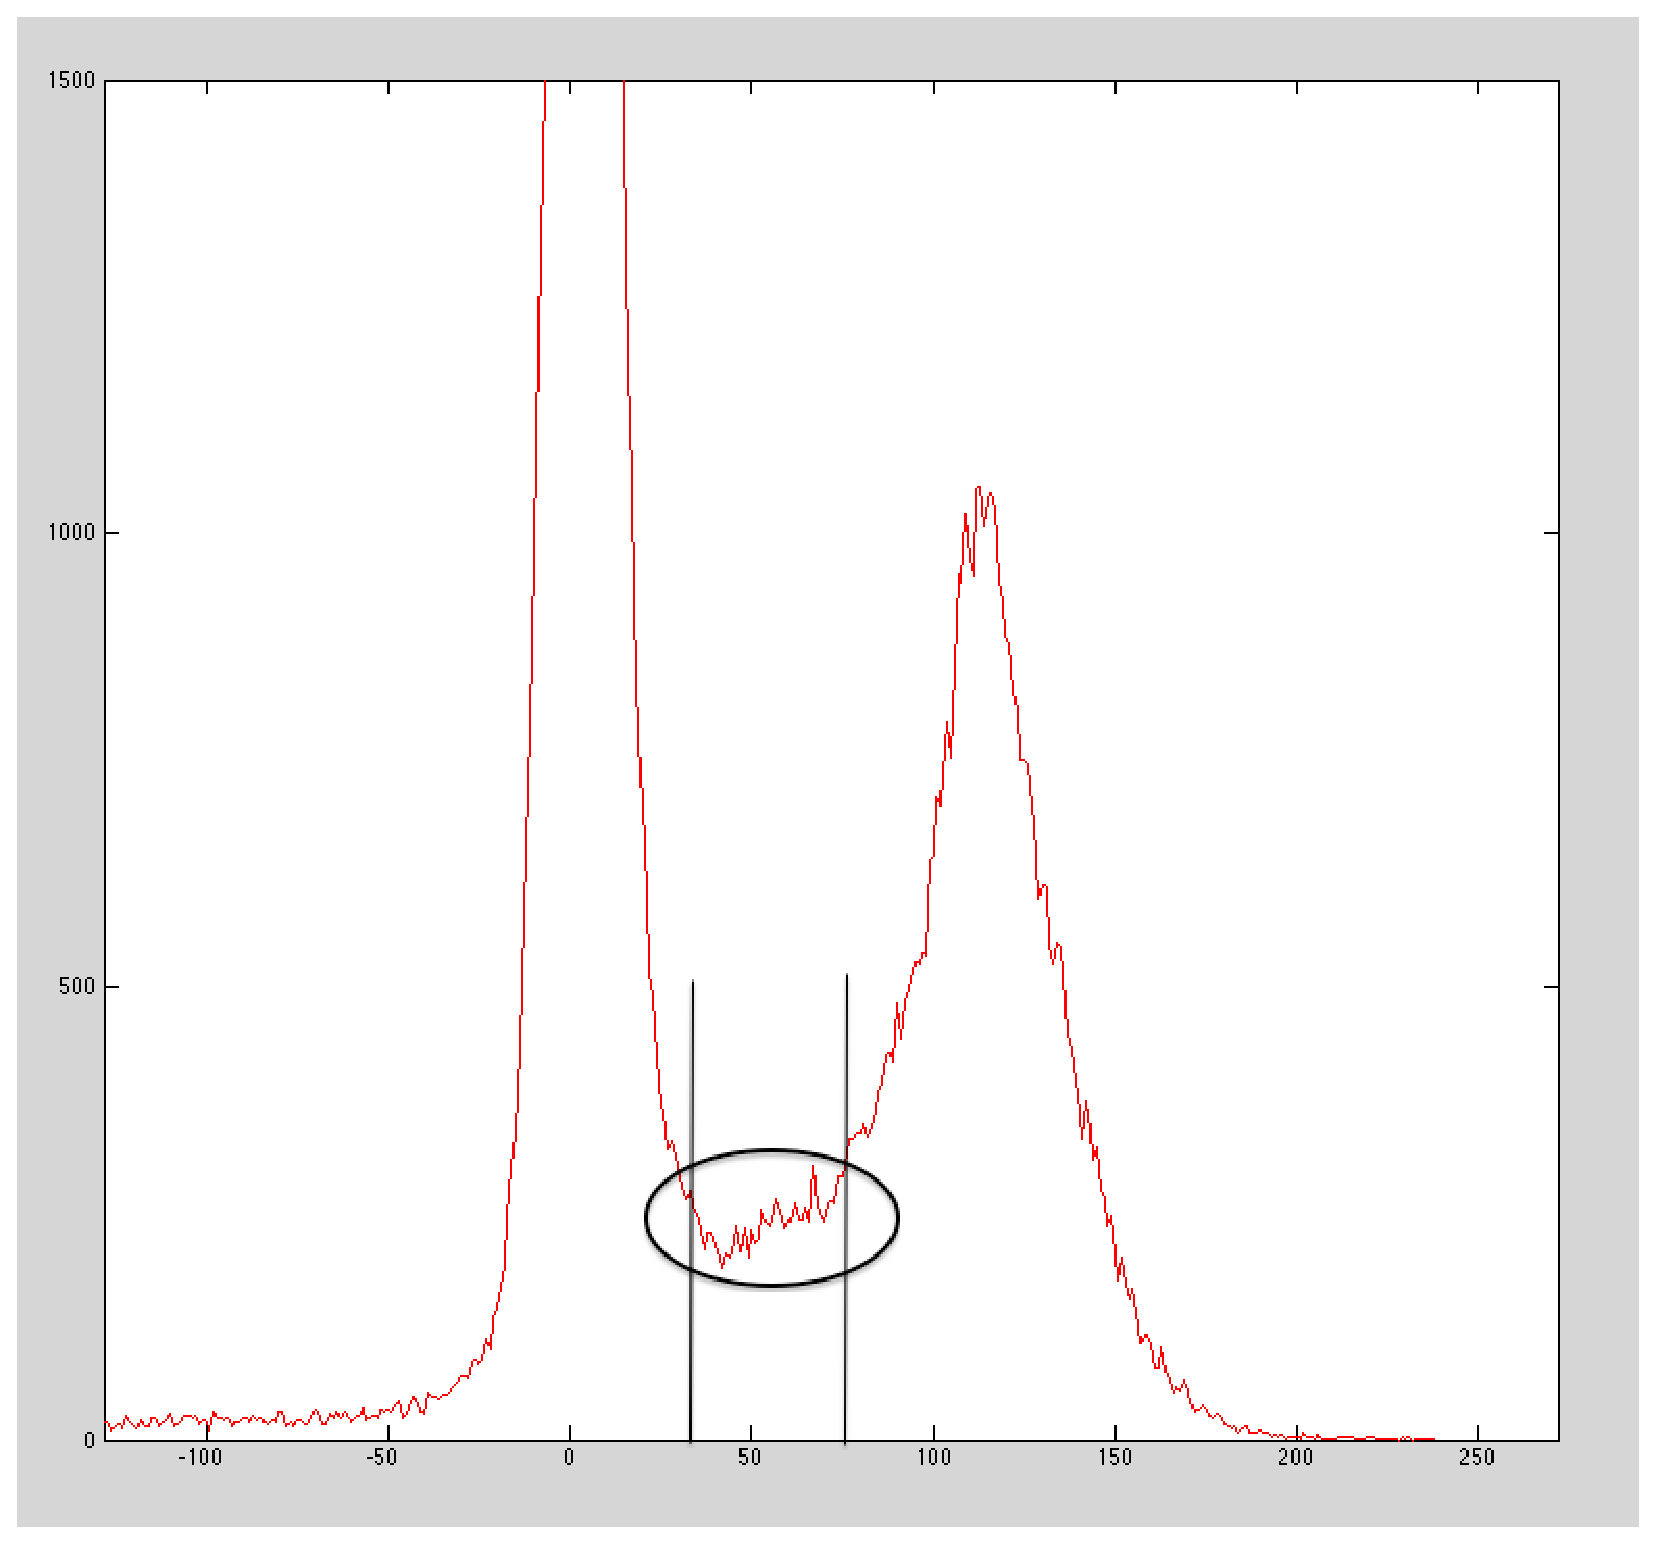
\includegraphics[width=2.75in]{data_extraction/images/mid_slice_tank_and_water_overlap_marked.eps}}}
    \centerline{\emph{(b) Mared overlap region}}
  \end{minipage}
  \begin{minipage}[t]{2.75in}
    \centering
    \centerline{\mbox{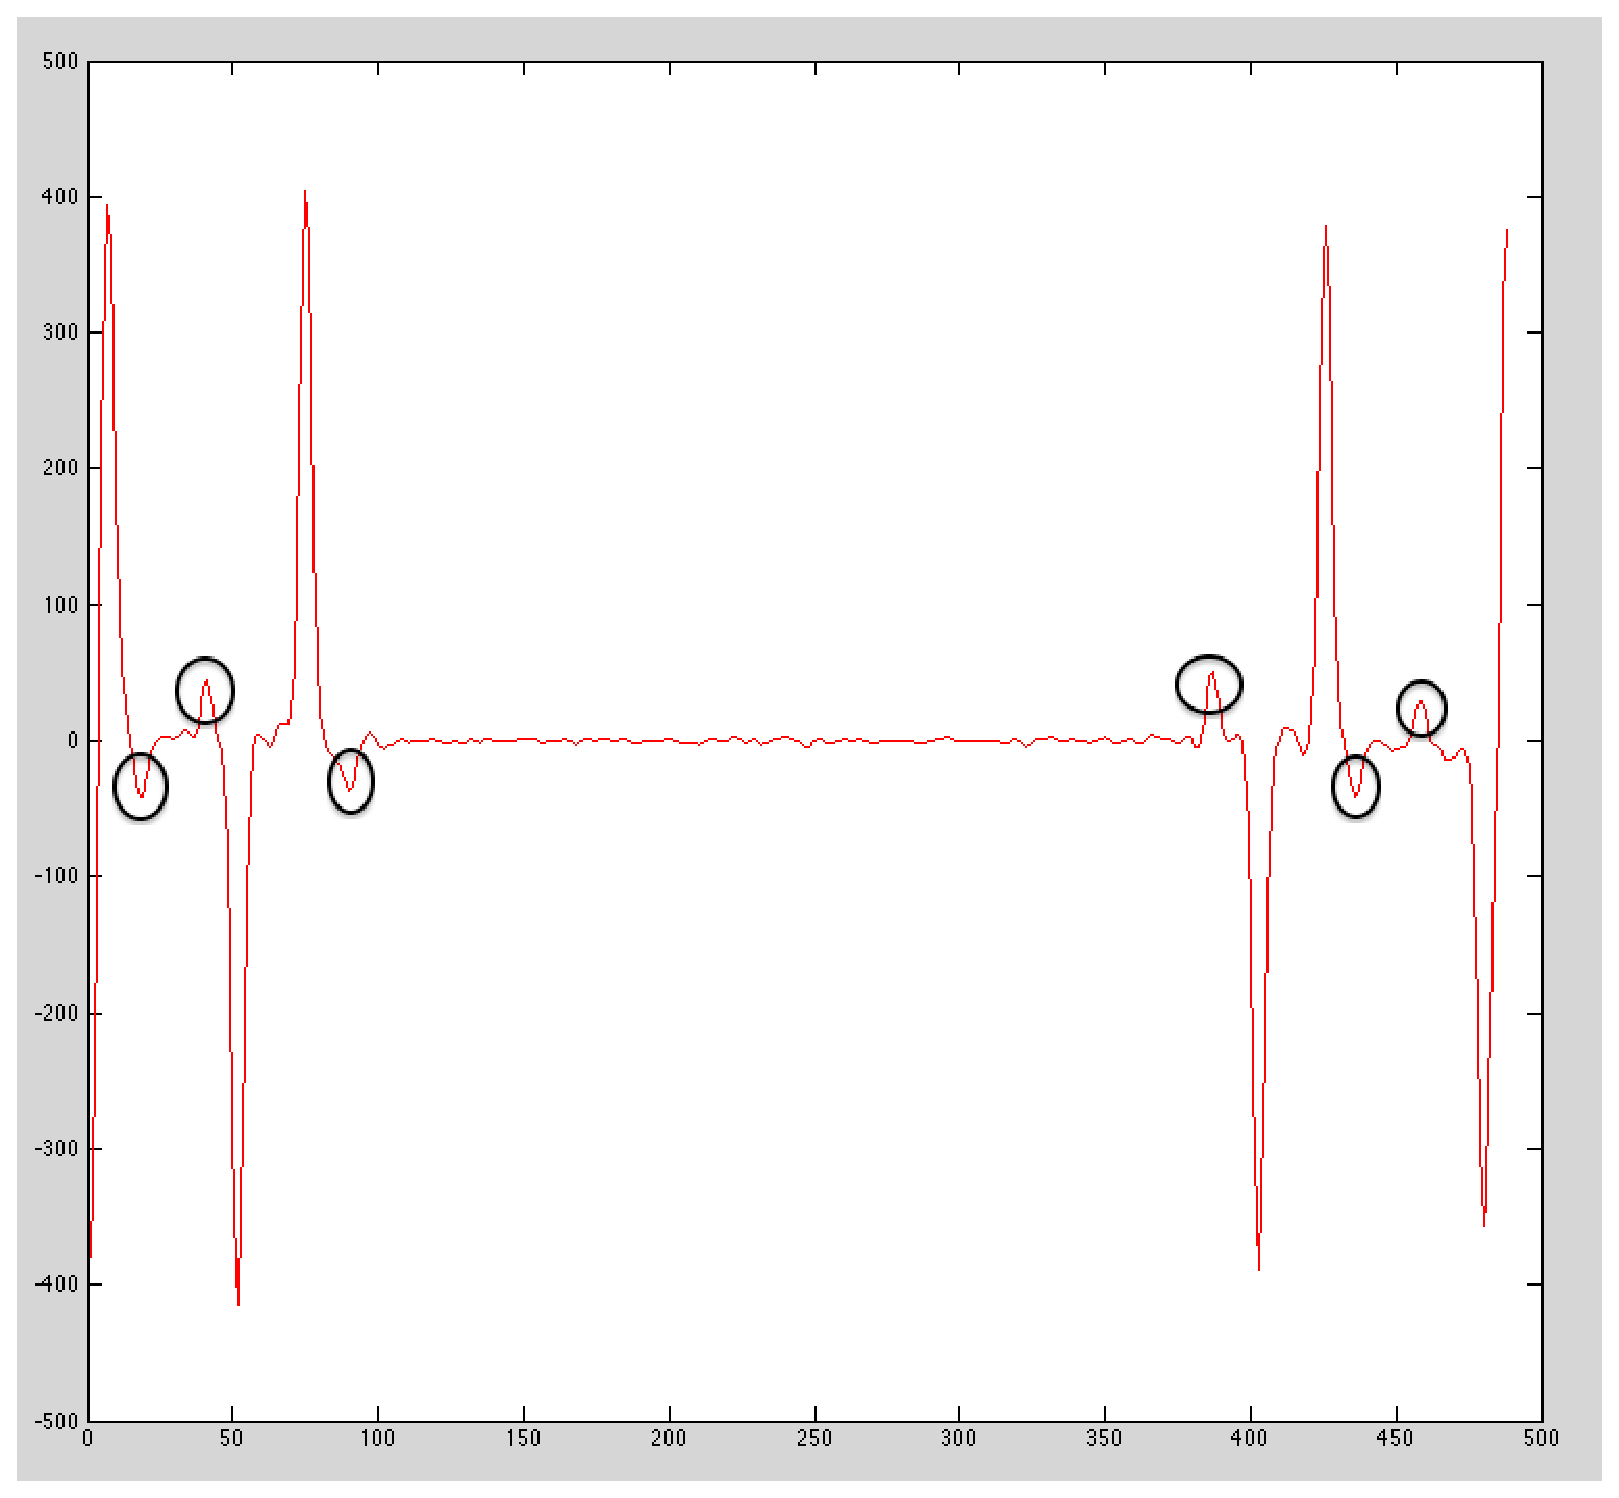
\includegraphics[width=2.75in]{data_extraction/images/mid_slice_gradient_marked.eps}}}
    \centerline{\emph{(c) mid slice surface locations}}
  \end{minipage}

  \caption{\emph{Histograms of middle column of middle slice of a coronal series}} 
  \label{fig:histograms_mid_coronal}
\end{figure}

\subsection{Edge Detection On Local Surface Region}

After the regions of boundaries of water and phantom tank are extract we can proceed to extract the surface
edge from these regions. The following issues are need to be resolved:
\begin{enumerate}
  \item Identify the left and right boundaries of the edges.
  \item Remove the noisy edges, and there are two types noisy edges:
    \begin{enumerate}
      \item Noisy edges that are not in contact with the target edge.
      \item Noisy edges that are in contact with the target edge.
    \end{enumerate}
\end{enumerate}

\subsubsection{Boundary Finding}

To detect the left and right boundary we plot the histogram of sum of intensities of each column across the
region as well as the gradient for the intensity graph as shown in figure 
\ref{fig:coronal_270_boundary_histogram}. 

\begin{figure}[htb]
  \begin{minipage}[t]{5in}
    \centering
    \centerline{\mbox{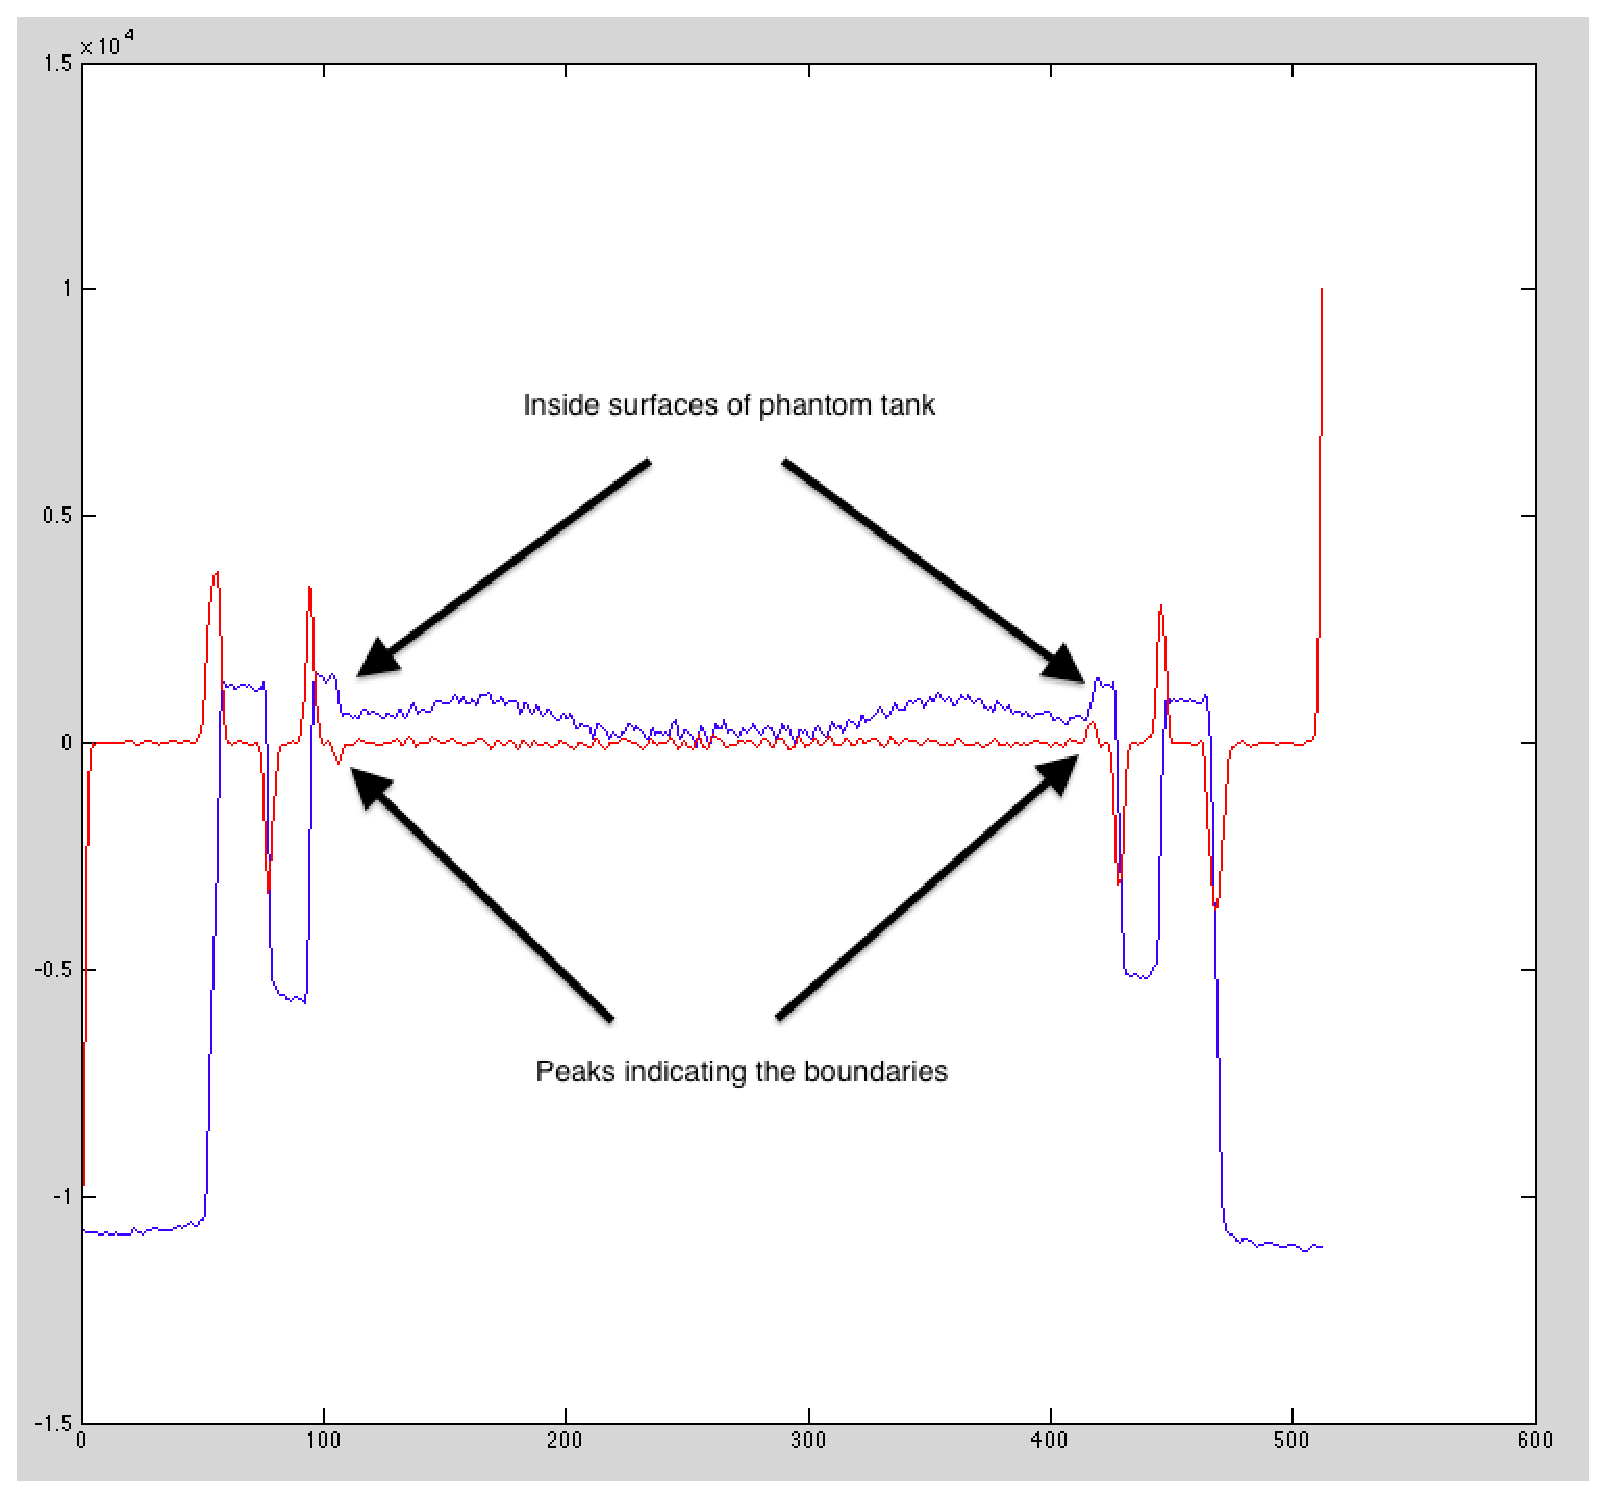
\includegraphics[width=5in]{data_extraction/images/sample/20121017_270/Coronal/inferior_inside/histogram_marked.eps}}}
    \centerline{\emph{(a) Histogram for inferior tank inside edge}}
  \end{minipage}
  \caption{\emph{Histogram for boundary detection on image sequence \#270}}
  \label{fig:coronal_270_boundary_histogram}
\end{figure}

\begin{figure}[htb]
  \begin{minipage}[t]{5in}
    \centering
    \centerline{\mbox{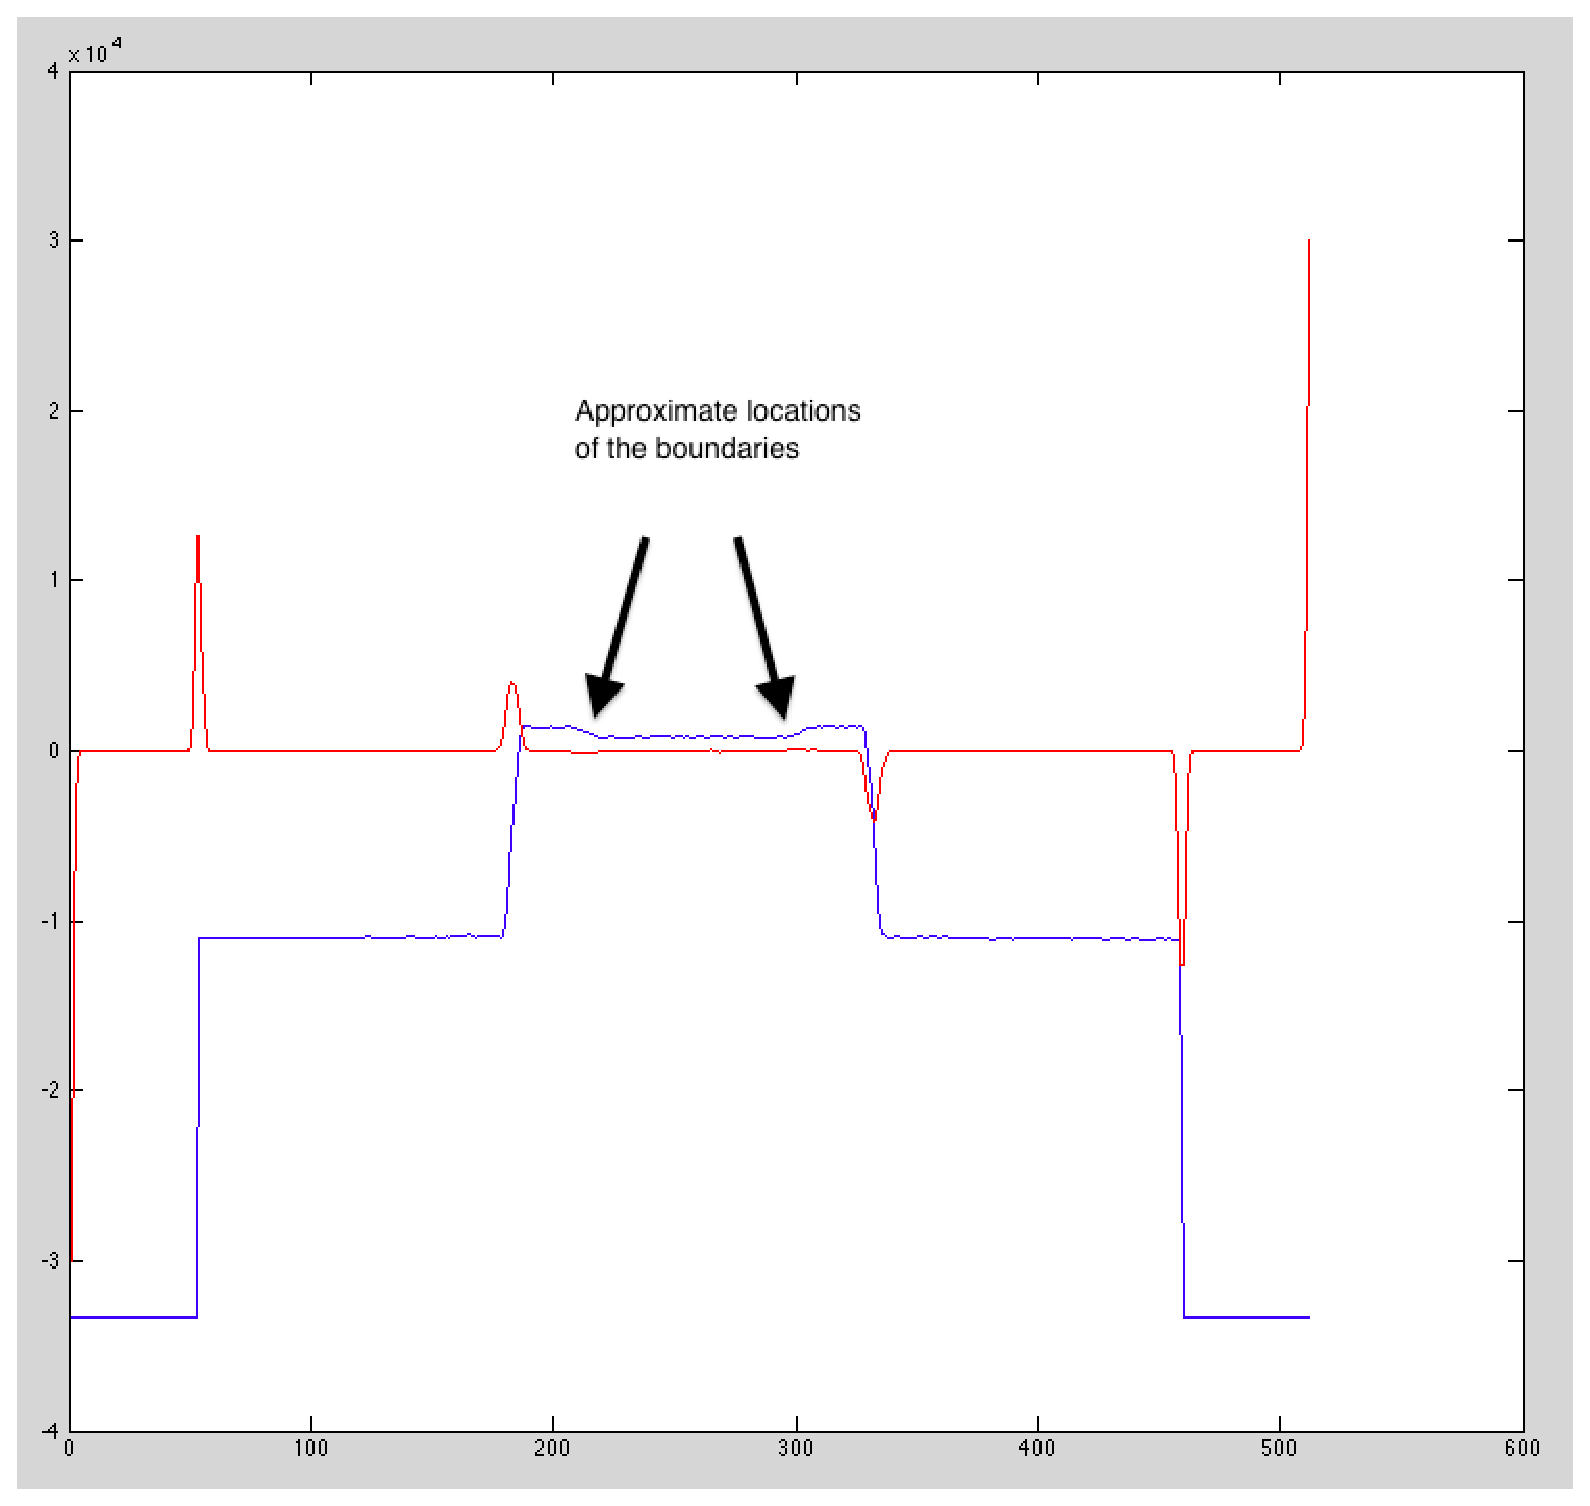
\includegraphics[width=5in]{data_extraction/images/sample/20121017_100/Coronal/superior_outside/superior_outside_histogram_marked.eps}}}
    \centerline{\emph{(a) Histogram for superior tank outside edge}}
  \end{minipage}
  \caption{\emph{Histogram for boundary detection on image sequence \#100}}
  \label{fig:coronal_270_boundary_histogram}
\end{figure}

Upper pair of arrows in figure \ref{fig:coronal_270_boundary_histogram} indicates where the inside edges of
the phantom tanks are, and the lower pair of arrows indicates how do those edges shows up in its gradient graph.
The two small edges are identifiable with properties of value bewteen 200 and 1000. We can identify them with
this property for most of the sliceds. The transition from phantom tank to water become smoother on the slices
more toward anterior or posterior in coronal view. 

There are couple of issues with this approach.
\begin{itemize}
  \item For images close to either edges of the two tanks, contrast ratio between water and tank material 
    become very weak. As shown in figure \ref{fig:coronal_edge_final_result}, the transition from tank to
    water become very smooth, and their gradient, therefore, become very small, and fallen out the filter
    range we specified. If we lower the range of the filter, it will pick up too many noise.
  \item For superior tank's outside surface, its regions also include the end part of tubes. Structure
    on those regions of tubes are fairly complex, which will result in frequent change of each column's 
    total intensities in regions that have tubes.
% so there are lots of change of peaks in the intensity 
%     graph as we can see in figure \ref{fig:superior_outside_artifacts}, and it's easy for some of these peaks to fall into the range of our
%     boundary filter. 
\end{itemize}

\begin{figure}[htb]
  \begin{minipage}[t]{2.75in}
    \centering
    \centerline{\mbox{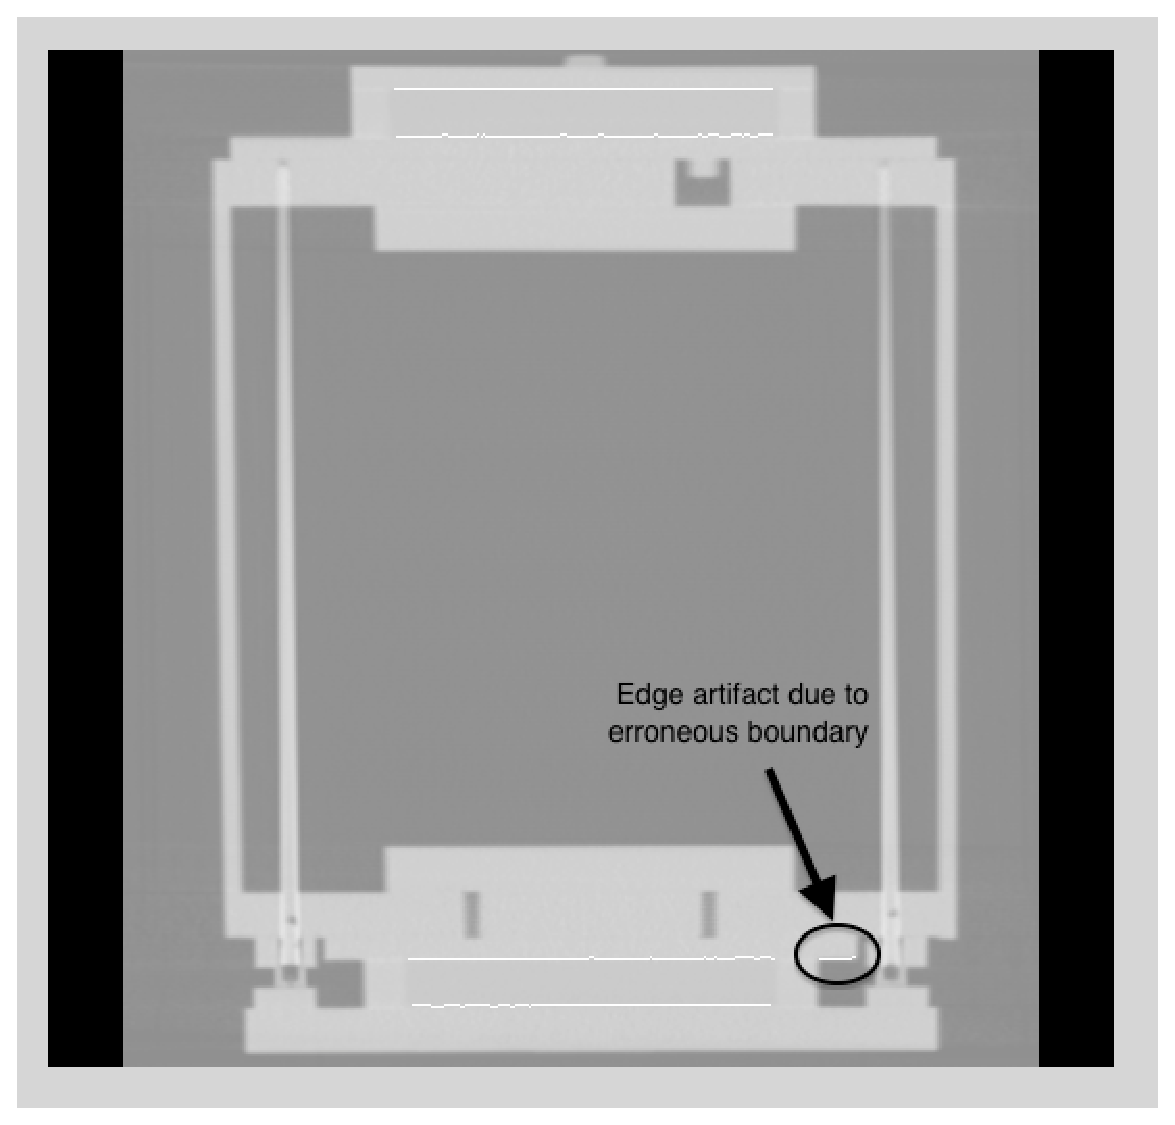
\includegraphics[width=2.75in]{data_extraction/images/sample/20121017_125/Coronal/Superior_outside/extra_edge.eps}}}
    \centerline{\emph{(a) Extra edge caused by tube section}}
  \end{minipage}
  \begin{minipage}[t]{2.75in}
    \centering
    \centerline{\mbox{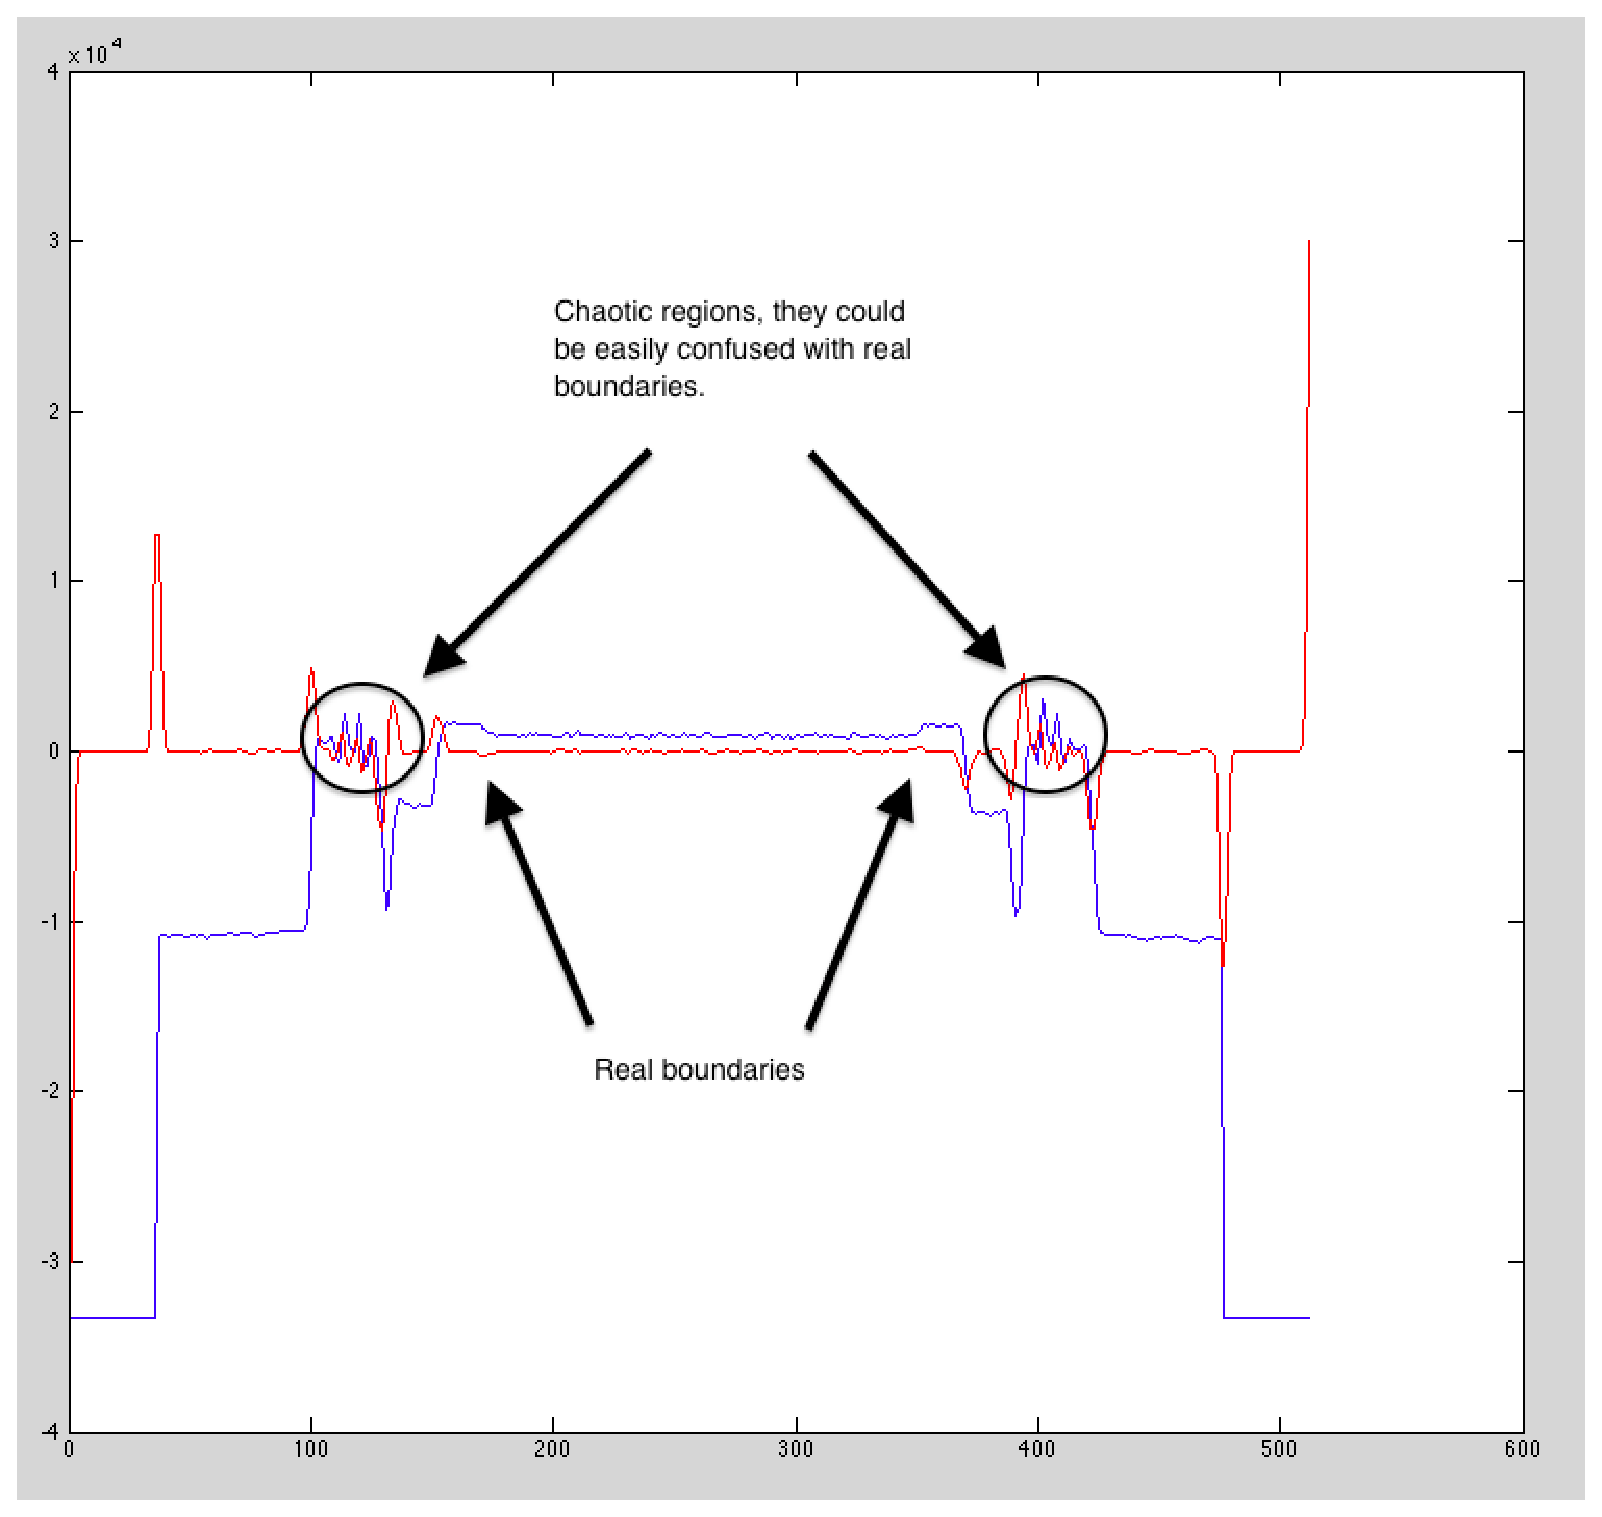
\includegraphics[width=2.75in]{data_extraction/images/sample/20121017_125/Coronal/Superior_outside/extra_edge_histogram.eps}}}
    \centerline{\emph{(b) Histgram of the superior outside surface in (a) }}
  \end{minipage}
  \caption{\emph{Superior outside surface artifacts}}
  \label{fig:superior_outside_artifacts}
\end{figure}

However, with the slices that able to identify the edges,
we can reconstruct majority of each water tank surface and they are more than enough for us to estimate the
distances between each surfaces, especially with the assumption that they are all flat and parallel to each
other.

\subsubsection{Removing Noise}

We are going to remove the noise of the each edge in two steps. 
\begin{enumerate}
  \item Remove noisy edges that are unattached to target edges.
  \item Filter out small edges sticking out of target edges. 
\end{enumerate}

Noisy edges unattached to target edges has one characteristic which is short. Since these edges are generated
by noises, all observations has shown that they all tend to be very short in length due to lack of consistent
pattern. To remove the noisy edges that are unattached to the target edges, we do the following steps:
\begin{enumerate}
  \item Create an empty image that has the same size of the input image.
  \item Iterate every pixel of input image
    \begin{enumerate}
      \item if current pixel in input image is not zero:
        \begin{enumerate}
          \item We recursively collect all the nonzero pixels from the input image and set those pixel values on
            the input image to 0.
        \end{enumerate}
      \item If there has been an edge collected, we check the length of this group of pixels
        \begin{enumerate}
          \item If the length is less than a threshold, say, 15, we assume they are a noisy edge and 
            complete ignore this group of pixels
          \item Otherwise, we will write these pixels' values to the image we initially created.
        \end{enumerate}
    \end{enumerate}
\end{enumerate}

After follwing above steps, the resulting image will look like something like figure 
\ref{fig:coronal_270_intermediate_results} (c).

At this stage, we will apply the boundary limit to this newly filtered edge, removing all the pixels beyond
either left or right boundary. And this will left us with target edges with some small noisy edges sticking
out as shown in figure \ref{fig:coronal_270_intermediate_results} (d).

To filter these sticking edges out, we do the following steps:

\begin{enumerate}
  \item Extract 2d coordinate informate of every edge pixels, and fit them to a straight line, since we know
    our target edge is a straight line. We can setup the equation as:
    \begin{eqnarray}
      \begin{bmatrix}
        columns \quad 1
      \end{bmatrix}
      \begin{bmatrix}
        m\\
        k\\
      \end{bmatrix}
      & = & 
      \begin{bmatrix}
        rows
      \end{bmatrix}
    \end{eqnarray}
    where \emph{columns} is column values of all edge pixels and \emph{rows} is row values of all edge pixels.
    $m$ and $k$ will the line parameter of the straight line we are trying to fit into.
  \item Group all edge pixels by their column value.
  \item Iterate all column groups. We pick a pixel from each group having the minimum value of
    $|Pixel_{row} - (m*Pixel_{column} + k)|$ and ignore the rest.
  \item At the end we should have one pixel per column group left, they will be our final edge.
\end{enumerate}

For testing we write out these filtered edges to original input image. We can see the result in figure 
\ref{fig:coronal_edge_final_result} (a). For some edges, in some image we are unable to determine the left
and right boundary. We will skip them as we have more than enough data with images that can gives us good 
edges. Figure Figure \ref{fig:coronal_edge_final_result} (b) is an example where some edges are identifiable
while others not.

\begin{figure}[htb]
  \begin{minipage}[t]{2.75in}
    \centering
    \centerline{\mbox{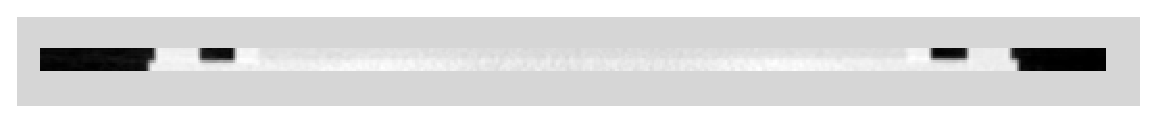
\includegraphics[width=2.75in]{data_extraction/images/sample/20121017_270/Coronal/inferior_inside/1_region.eps}}}
    \centerline{\emph{(a) Extracted region}}
  \end{minipage}\medskip
  \begin{minipage}[t]{2.75in}
    \centerline{\mbox{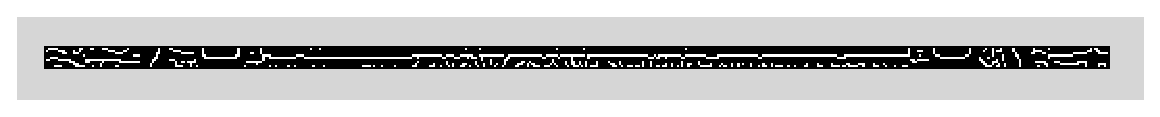
\includegraphics[width=2.75in]{data_extraction/images/sample/20121017_270/Coronal/inferior_inside/2_raw_edges.eps}}}
    \centerline{\emph{(b) Raw edges}}
  \end{minipage}
  \begin{minipage}[t]{2.75in}
    \centerline{\mbox{\includegraphics[width=2.75in]{data_extraction/images/sample/20121017_270/Coronal/inferior_inside/3_removed_noise.eps}}}
    \centerline{\emph{(c) Removed noisy edges}}
  \end{minipage}\medskip
  \begin{minipage}[t]{2.75in}
    \centerline{\mbox{\includegraphics[width=2.75in]{data_extraction/images/sample/20121017_270/Coronal/inferior_inside/4_within_boundary.eps}}}
    \centerline{\emph{(d) Edges within the boundary}}
  \end{minipage}
  \caption{\emph{Edge extraction intermediate results on image sequence \#270's inferior tank inside edge}}
  \label{fig:coronal_270_intermediate_results}
\end{figure}

\subsubsection{Improvement}



\begin{figure}[htb]
  \begin{minipage}[t]{2.75in}
    \centering
    \centerline{\mbox{\includegraphics[width=2.75in]{data_extraction/images/sample/20121017_270/Coronal/result.eps}}}
    \centerline{\emph{(a) Edge result on image sequence \#270}}
  \end{minipage}
  \begin{minipage}[t]{2.75in}
    \centering
    \centerline{\mbox{\includegraphics[width=2.75in]{data_extraction/images/sample/20121017_100/Coronal/result_canny_[0.001,0.002].eps}}}
    \centerline{\emph{(b) Edge result on image sequence \#100}}
  \end{minipage}
  \caption{\emph{Final edge results}}
  \label{fig:coronal_edge_final_result}
\end{figure}


\subsection{Creating Surfaces}

Surface in 3D space can be represented by equation:
\begin{eqnarray}
ax + by + cz + d & = & 0 \label{eq:plane}
\end{eqnarray}

With somewhere between 50,000~70,000 date points for each surfaces, it's the best to use least square ($Ax=b$) to 
esitmate each surfaces' equation paramters. Considering the following fact:
\begin{enumerate}
  \item Least square assumes that there is error in measurement but not observation, so it will only try to
    minimize error in A not b.
  \item For every data point we only have measurement error in two axis, the third one is taking for granted 
    from DICOM info. Though there should be some very small error during CT image reconstruction as well, but
    that's not necessary to be consider here.
\end{enumerate}
Since the image set we are dealing with is coronal view, which means it's the y-axis we are taking for granted,
we are setting up our least square as follows:

\begin{eqnarray}
\frac{a}{b}x + \frac{c}{b}z + \frac{d}{b} & = & -y \label{eq:x_orient}\\
\begin{bmatrix}
  x_0  & z_0 & 1 \\
  \vdots & \vdots & \vdots \\
  x_n & z_n & 1 \\
\end{bmatrix}
\begin{bmatrix}
a/b\\
c/b\\
d/b
\end{bmatrix}
& = &
\begin{bmatrix}
-y_0 \\
\vdots\\
-y_n
\end{bmatrix}
\end{eqnarray}

With this setup, our estimated paramters for each planes are:

\begin{tabular}{| l || r | r | r | r |}
            \hline
            &               $a$ & $b$ &               $c$ & $d$ \\
            \hline
  surface 1 & $-1.0617\times10^{-06}$ & $1$ & $-6.9880\times10^{-10}$ & $-2.0644$ \\ 
            \hline
  surface 2 & $-3.8209\times10^{-06}$ & $1$ & $-2.3851\times10^{-9}$  & $-6.7681$ \\ 
            \hline
  surface 3 & $3.2496\times10^{-06}$  & $1$ & $4.3242\times10^{-10}$  & $-4.8297$ \\ 
            \hline
  surface 4 & $3.3399\times10^{-06}$  & $1$ & $1.2575\times10^{-10}$  & $-2.0644$ \\ 
            \hline
\end{tabular}

% algorithm limited by two factors:
% \begin{enumerate}
%   \item left and right boundary finding
%   \item canny parameters
% \end{enumerate}

% continue here $\dots$

Reconstructed surfaces can be see below:

\begin{figure}[htb]
  \begin{minipage}[t]{2.75in}
    \centering
    \centerline{\mbox{\includegraphics[width=2.75in]{data_extraction/images/surface_plane/superior_comparison/Surface1_2.eps}}}
    \centerline{\emph{(a)}}
  \end{minipage}\medskip
  \begin{minipage}[t]{2.75in}
    \centering
    \centerline{\mbox{\includegraphics[width=2.75in]{data_extraction/images/surface_plane/inferior_comparison/Surface3_4.eps}}}
    \centerline{\emph{(b)}}
  \end{minipage}
  \begin{minipage}[t]{2.75in}
    \centering
    \centerline{\mbox{\includegraphics[width=2.75in]{data_extraction/images/surface_plane/Surface1_2_3_4.eps}}}
    \centerline{\emph{(c)}}
  \end{minipage}\medskip
  \begin{minipage}[t]{2.75in}
    \centering
    \centerline{\mbox{\includegraphics[width=2.75in]{data_extraction/images/surface_plane/saggital_ct_tilt.eps}}}
    \centerline{\emph{(d)}}
  \end{minipage}
  
  \caption{\emph{Water tank surfaces reconstruction from CT scan, YZ view}}
  \label{fig:ct_tank_surface_reconstruction_yz}

\end{figure}

\begin{figure}[htb]
  \begin{minipage}[t]{2.75in}
    \centering
    \centerline{\mbox{\includegraphics[width=2.75in]{data_extraction/images/surface_plane/superior_inside/xy.eps}}}
    \centerline{\emph{(a)}}
  \end{minipage}\medskip
  \begin{minipage}[t]{2.75in}
    \centering
    \centerline{\mbox{\includegraphics[width=2.75in]{data_extraction/images/surface_plane/superior_outside/xy.eps}}}
    \centerline{\emph{(b)}}
  \end{minipage}
  \begin{minipage}[t]{2.75in}
    \centering
    \centerline{\mbox{\includegraphics[width=2.75in]{data_extraction/images/surface_plane/inferior_inside/xy.eps}}}
    \centerline{\emph{(c)}}
  \end{minipage}\medskip
  \begin{minipage}[t]{2.75in}
    \centering
    \centerline{\mbox{\includegraphics[width=2.75in]{data_extraction/images/surface_plane/inferior_outside/xy.eps}}}
    \centerline{\emph{(d)}}
  \end{minipage}
  \caption{\emph{Water tank surfaces reconstruction from CT scan, XY view}}
  \label{fig:ct_tank_surface_reconstruction_xy}
\end{figure}

Notice that in the YZ view in figure \ref{fig:ct_tank_surface_reconstruction_yz}(a) (b) (c), 
all four surfaces are tilted. This is consistant with what we observed on saggital reconstruction 
of this image set. 

\subsection{Estimating Surfaces Distances}


\Chapter{Parameters Calculation}
\label{parameters_calculation}
\section{Introduction}
With both original measurements of the phantom and distorted data points, distortion or correction 
parameters can now be calculated 

\begin{eqnarray} \label{eq:spherical_harmonics}
\bar{x_i} = x_i(1 + K_{x_0}(x_i^2 + y_i^2) + K_{x_1}z_i^2 + K_{x_2}z_i^2(x_i^2 + y_i^2) 
+ K_{x_3}(x_i^2 + y_i^2)^2 + K_{x_4}z_i^4) \\
\bar{y_i} = y_i(1 + K_{y_0}(x_i^2 + y_i^2) + K_{y_1}z_i^2 + K_{y_2}z_i^2(x_i^2 + y_i^2) 
+ K_{y_3}(x_i^2 + y_i^2)^2 + K_{y_4}z_i^4) \\
\bar{z_i} = z_i(1 + K_{z_0}(x_i^2 + y_i^2) + K_{z_1}z_i^2 + K_{z_2}z_i^2(x_i^2 + y_i^2) 
+ K_{z_3}(x_i^2 + y_i^2)^2 + K_{z_4}z_i^4)
\end{eqnarray}

where $(\bar{x}_i, \bar{y}_i, \bar{z}_i)$ and $(x_i, y_i, z_i)$ represent distorted and corrected data sets.
If $(\bar{x}_i, \bar{y}_i, \bar{z}_i)$ is distorted data set, $K_{x_i}, K_{y_i}, K_{z_i}$ would be 
distortion parameters, i.e. parameters used to distort original phantom data. If 
$(\bar{x}_i, \bar{y}_i, \bar{z}_i)$ and $(x_i, y_i, z_i)$ are swapped, $K_{x_i}, K_{y_i}, K_{z_i}$ would work as
correction parameters, i.e. parameters used to convert distorted data points into their original position.
In this case, what need to be calculated is correction parameters which will be used to correct the
distortions inside MR images.

Both $(x_i, y_i, z_i)$ and $(\bar{x}_i, \bar{y}_i, \bar{z}_i)$ have to be in DICOM coordinate, i.e. relative
coordinate from gradient isocenter. The gradient isocenter computed in early chapters are using data points
extracted from MR images, so it can be used to convert data points from MR images into DICOM coordinate, but 
not the corrected data. 

\section{XY Axis Distortion Correction Parameters Calculation}
This section describes how to setup and calculate the X and Y axis correction parameters.

Consider using two data points from two separate MR tubes in the same xy plane, two equations could be
setup:

\begin{eqnarray} \label{eq:xy_setup_sample}
\bar{x_0} = x_0(1 + K_{x_0}(x_0^2 + y_0^2) + K_{x_1}z_0^2 + K_{x_2}z_0^2(x_0^2 + y_0^2) 
+ K_{x_3}(x_0^2 + y_0^2)^2 + K_{x_4}z_0^4)  \\
\bar{x_1} = x_1(1 + K_{x_1}(x_1^2 + y_1^2) + K_{x_1}z_1^2 + K_{x_2}z_1^2(x_1^2 + y_1^2) 
+ K_{x_3}(x_1^2 + y_1^2)^2 + K_{x_4}z_1^4) 
\end{eqnarray}

where $(x_0, y_0, z_0)$ and $(x_1, y_1, z_1)$ are DICOM coordinates of the two points from distorted space, 
which are known, and $(\bar{x}_0, \bar{y}_0, \bar{z}_0)$, $(\bar{x}_1, \bar{y}_1, \bar{z}_1)$ are DICOM 
coordinates of two points from corrected spaces which are unknown. However, the exact distance of tube
spacings are known, as well as the distance between opposite side of tubes. So 
$(\delta{x}_{0,1}, \delta{y}_{0,1}, \delta{z}_{0,1})$ can be calculated using 

\begin{equation}
  (\delta{x}_{i,j}, \delta{y}_{i,j}, \delta{z}_{i,j}) = 
  (\bar{x}_i, \bar{y}_i, \bar{z}_i) - (\bar{x}_j, \bar{y}_j, \bar{z}_j)
\end{equation}

where $i, j$ should belong to the same row of tubes for calculating X-axis correction parameters 
or should belong to the same column of tubes for calculating Y-axis correction parameters. 
figure \ref{fig:correction_tube_pairing_xy} shows how the pairing is done for x, and y axis. 

\begin{figure}[htb]
  \begin{center}
    \begin{minipage}[b]{2.6in}
      \centering
      \centerline{\mbox{\includegraphics[width=2.6in]{parameters/images/tubes_pairing_x.eps}}}
      \centerline{\emph{(a)}}
    \end{minipage}
    \begin{minipage}[b]{2.6in}
      \centering
      \centerline{\mbox{\includegraphics[width=2.6in]{parameters/images/tubes_pairing_y.eps}}}
      \centerline{\emph{(b)}}
    \end{minipage}
  \end{center}
  \caption{Pairing of MR tubes. (a) Pairing for X-axis (b) Pairing for Y-axis}
  \label{fig:correction_tube_pairing_xy}
\end{figure}

For each pairing, a new formula is produced.
\begin{eqnarray} 
  \delta{\bar{x_{ij}}} & = & \delta{x_{ij}}(1 + K_{x_0}((x_i^2 + y_i^2) - (x_j^2 + y_j^2)) + \nonumber\\
  & & K_{x_1}(z_i^2 - z_j^2) + \nonumber\\
  & & K_{x_2}(z_i^2(x_i^2 + y_i^2)- z_j^2(x_j^2 + y_j^2)) + \nonumber\\
  & & K_{x_3}((x_i^2 + y_i^2)^2 - (x_j^2 + y_j^2)^2) + \nonumber\\
  & & K_{x_4}(z_0^4 - z_j^4)) \\
  \delta{\bar{y_{ij}}} & = & \delta{y_{ij}}(1 + K_{y_0}((x_i^2 + y_i^2) - (x_j^2 + y_j^2)) + \nonumber\\
  & & K_{y_1}(z_i^2 - z_j^2) + \nonumber\\
  & & K_{y_2}(z_i^2(x_i^2 + y_i^2)- z_j^2(x_j^2 + y_j^2)) + \nonumber\\
  & & K_{y_3}((x_i^2 + y_i^2)^2 - (x_j^2 + y_j^2)^2) + \nonumber\\
  & & K_{y_4}(z_0^4 - z_j^4))
\end{eqnarray}

\section{Z Axis Distortion Correction Parameters Calculation}

Similarly to xy correction, we pair up surfaces of water tanks. Figure \ref{fig:correction_surface_pairing}, 
show the pairing. \\

\begin{figure}[htb]
  \begin{center}
    \begin{minipage}[b]{3in}
      \centering
      \centerline{\mbox{\includegraphics[width=3in]{parameters/images/surface_pairing_z.eps}}}
      % \centerline{\emph{(a)}}
    \end{minipage}
  \end{center}
  \caption{Pairing of tank surfaces. }
  \label{fig:correction_surface_pairing}
\end{figure}

And the formula we used for z axis correction is:
\begin{eqnarray}
  \delta{\bar{z_{ij}}} & = & \delta{z_{ij}}(1 + K_{z_0}((x_i^2 + y_i^2) - (x_j^2 + y_j^2)) + \nonumber\\
  & & K_{z_1}(z_i^2 - z_j^2) + \nonumber\\
  & & K_{z_2}(z_i^2(x_i^2 + y_i^2)- z_j^2(x_j^2 + y_j^2)) + \nonumber\\
  & & K_{z_3}((x_i^2 + y_i^2)^2 - (x_j^2 + y_j^2)^2) + \nonumber\\
  & & K_{z_4}(z_0^4 - z_j^4))  
\end{eqnarray}

% \subsubsection{Accuracy}

% The accuracy has been tested in matlab simulation. XY axis correction tends to stay around within 0.001 mm
% while Y axis correction is around 0.1mm accuracy.



% \Chapter{Verification}
\Chapter{Summery and Conclusion}

\bibliographystyle{plain}
\bibliography{thesis}
\end{document}
